\باب{تکمل}
اس باب میں دو اعمال اور ان کا ایک دوسرے کے ساتھ تعلق پر غور کیا جائے گا۔ پہلے عمل میں  ہم تفرق سے تفاعل  حاصل کرتے ہیں۔ دوسرے عمل میں ہم حجم، رقبہ، وغیرہ کے بالکل درست کلیات، بذریعہ یک بعد دیگرے تخمین، دریافت کرتے ہیں۔ ان دونوں اعمال کو تکمل کہتے ہیں۔

تکمل اور تفرق کا گہرا تعلق ہے۔ یہ تعلق تمام ریاضیات میں اہم ترین حقائق میں سے ایک ہے۔ لیبنٹز اور نیوٹن نے علیحدہ علیحدہ اس تعلق کو دریافت کیا۔

\حصہ{غیر قطعی تکملات}
کسی جسم کے موجودہ مقام اور سمتی رفتار سے اس کے مستقبل کے  مقام کی پیش گوئی کرنا احصاء کی اولین کامیابیوں میں سے ایک تھی۔ آج کل تفاعل کی کسی  ایک معلوم قیمت اور شرح تبدیلی سے تفاعل کے دیگر قیمتوں کا حصول معمول کی بات ہے۔ہم احصاء کی مدد سے  کشش زمین سے نکلنے کے لئے درکار رفتار یا تابکار مادہ کی موجودہ عملیت اور شرح تابکاری تحلیل سے اس کی قابل استعمال زندگی کا حساب لگا سکتے ہیں۔

تفاعل کی معلوم قیمتوں میں سے کسی ایک قیمت اور تفاعل کے تفرق \عددی{f(x)} سے تفاعل کا حصول دو قدموں میں ممکن ہے۔ پہلے قدم میں وہ تمام تفاعل حاصل کیے جاتے ہیں جن کا تفرق \عددی{f} ہے۔ ان تفاعل کو \عددی{f} کے الٹ تفرقات کہتے ہیں اور جس کلیہ سے انہیں اخذ کیا جاتا ہے اس کو \عددی{f} کا غیر قطعی  تکمل  کہتے ہیں۔ دوسرے قدم میں تفاعل کی معلوم قیمت استعمال کرتے ہوئے الٹ تفرقات میں سے مخصوص تفاعل منتخب کیا جاتا ہے۔ اس حصہ میں پہلے قدم پر غور کیا جائے گا جبکہ دوسرے قدم پر اگلے حصہ میں غور کیا جائے گا۔

اگرچہ تفاعل کے تمام الٹ تفرقات حاصل کرنے والا کلیہ دریافت کرنا  ناممکن نظر آتا ہے، حقیقت میں ایسا نہیں ہے۔ مسئلہ اوسط قیمت (مسئلہ \حوالہ{مسئلہ_استعمال_اوسط_قیمت}) کے  پہلا اور دوسرا ضمنی نتائج کی مدد سے تفاعل کے  ایک الٹ تفرق سے اس کے تمام الٹ تفرقات حاصل کیے جا سکتے ہیں۔ 

\جزوحصہء{الٹ تفرق کا حصول۔ غیر قطعی تکمل}
\ابتدا{تعریف}
تفاعل \عددی{f(x)} کا  الٹ تفرق تب \عددی{F(x)} ہو گا جب \عددی{f} کے دائرہ کار میں تمام \عددی{x} کے لئے درج ذیل مطمئن ہوتا ہو۔
\begin{align*}
F'(x)=f(x)
\end{align*}
\عددی{f} کے تمام الٹ تفرقات کا سلسلہ \عددی{x} کے لحاظ سے \عددی{f} کا \اصطلاح{غیر قطعی تکمل}\فرہنگ{تکمل!غیر قطعی}\حاشیہب{indefinite integral}\فرہنگ{integral!indefinite} ہو گا جس کو درج ذیل سے ظاہر کیا جاتا ہے۔
\begin{align*}
\int f(x)\dif x
\end{align*}
علامت \عددی{\int} کو \اصطلاح{علامت تکمل} کہتے ہیں۔ تفاعل \عددی{f} کو \اصطلاح{متکمل}\فرہنگ{متکمل}\حاشیہب{integrand}\فرہنگ{integrand} اور \عددی{x} کو \اصطلاح{تکمل کا متغیر}\فرہنگ{تکمل!متغیر}\حاشیہب{variable of integration}\فرہنگ{integration!variable} کہتے ہیں۔
\انتہا{تعریف}
%======================

مسئلہ اوسط قیمت (مسئلہ \حوالہ{مسئلہ_استعمال_اوسط_قیمت}) کے  دوسرے ضمنی نتیجہ کے تحت تفاعل \عددی{f} کے  حاصل کردہ الٹ تفرق \عددی{F} اور اس کے  کسی دوسرے الٹ تفرق  میں صرف مستقل کا فرق پایا جائے گا۔ اس حقیقت کو تکملی علامتیت میں ظاہر کرتے ہیں:
\begin{align}\label{مساوات_تکمل_غیر_قطعی_الف}
\int f(x)\dif x=F(x)+C
\end{align}
مستقل \عددی{C} کو \اصطلاح{تکمل کا مستقل}\فرہنگ{تکمل!کا مستقل}\حاشیہب{constant of integration}\فرہنگ{integration!constant of} یا  \اصطلاح{اختیاری مستقل}\فرہنگ{مستقل!اختیاری}\حاشیہب{arbitrary constant}\فرہنگ{constant!arbitrary} کہتے ہیں۔ ہم مساوات \حوالہ{مساوات_تکمل_غیر_قطعی_الف} کو یوں پڑھتے ہیں: "\عددی{x} کے لحاظ سے تفاعل \عددی{f} کا غیر قطعی تکمل \عددی{F(x)+C} ہے۔"  \عددی{F(x)+C} کے حصول کو \عددی{f} کے \اصطلاح{تکمل} کا حصول کہتے ہیں۔

\ابتدا{مثال}
\عددی{\int 2x\dif x} تلاش کریں۔\\
حل:
\begin{align*}
\int 2x\dif x=x^2+C
\end{align*}
\عددی{2x} کا الٹ تفرق \عددی{x^2} ہے اور \عددی{C} تکمل کا مستقل ہے۔کلیہ \عددی{x^2+C} تفاعل \عددی{2x} کے تمام تفرقات دیتا ہے۔یوں \عددی{x^2+1}، \عددی{x^2-\pi} اور \عددی{x^2+\sqrt{2}} تفاعل \عددی{2x} کے ممکنہ الٹ تفرق ہیں۔ آپ ان کا تفرق لے کر تصدیق کر سکتے ہیں۔
\انتہا{مثال}
%======================

ہم عموماً تفرق کے کلیات سے الٹ تفرقات کے کلیات اخذ کرتے ہیں۔جدول \حوالہ{جدول_تکمل_کلیات_الف} میں غیر قطعی تکملات کے سامنے موزوں تفرقی کلیات کو الٹ لکھا گیا ہے۔ 
\begin{table}
\caption{تکمل کے کلیات}
\label{جدول_تکمل_کلیات_الف}
\centering
\renewcommand{\arraystretch}{2} 
\begin{tabular}{@{}LLL@{}}
\toprule
&\text{\RL{غیر قطعی تکمل}}&\text{\RL{تفرقی کلیات کو الٹ لکھا گیا ہے}}\\ 
\midrule
1.&{\displaystyle \int x^n\dif x=\frac{x^{n+1}}{n+1}+C}, \quad n\ne -1, \,n\text{ناطق} &\frac{\dif}{\dif x}\big(\frac{x^{n+1}}{n+1}\big)=x^n\\ 
&{\displaystyle \int \dif x=\int 1\dif x=x+C} \quad \text{\RL{(خصوصی صورت)}}&\frac{\dif}{\dif x}(x)=1\\ 
2.&{\displaystyle \int\sin kx\dif x=-\frac{\cos kx}{k}+C}&\frac{\dif}{\dif x}(-\frac{\cos kx}{k})=\sin kx\\ 
3.&{\displaystyle \int\cos kx\dif x=\frac{\sin kx}{k}+C}&\frac{\dif}{\dif x}(\frac{\sin kx}{k})=\cos kx\\ 
4.&{\displaystyle\int\sec^2x\dif x=\tan x+C}&\frac{\dif}{\dif x}\tan x=\sec^2x\\ 
5.&{\displaystyle\int\csc^2x\dif x=-\cot x+C}&\frac{\dif}{\dif x}(-\cot x)=\csc^2x \\ 
6.&{\displaystyle\int\sec x\tan x\dif x=\sec x+C}&\frac{\dif}{\dif x}\sec x=\sec x \tan x\\ 
7.&{\displaystyle\int\csc x\cot x\dif x=-\csc x+C}&\frac{\dif}{\dif x}(-\csc x)=\csc x\cot x\\
\bottomrule
\end{tabular}
\end{table}

\ابتدا{مثال}
\begin{enumerate}[a.]
\item
 جدول \حوالہ{جدول_تکمل_کلیات_الف} کے کلیہ 1 میں $n=5$ لیتے ہوئے:
\begin{align*}\int x^5\dif x=\frac{x^6}{6}+C\end{align*}

\item
کلیہ 1 میں \عددی{n=-\tfrac{1}{2}} لیتے ہوئے:
\begin{align*}\int \frac{1}{\sqrt{x}}\dif x=\int x^{-\tfrac{1}{2}}\dif x=2x^{\tfrac{1}{2}}+C\end{align*}

\item
کلیہ 2 میں \عددی{k=2} لیتے ہوئے:
\begin{align*}\int\sin 2x\dif x=-\frac{\cos 2x}{2}+C\end{align*}

\item
کلیہ 3 میں \عددی{k=\tfrac{1}{2}} لیتے ہوئے:
\begin{align*}\int\cos \frac{x}{2}\dif x=\int\frac{1}{2}x\dif x=\frac{\sin \tfrac{1}{2}x}{\tfrac{1}{2}}+C=2\sin\frac{x}{2}+C\end{align*}
\end{enumerate}
\انتہا{مثال}
%================

بعض اوقات کلیہ تکمل کا حصول مشکل ثابت ہوتا ہے البتہ  اخذ کردہ کلیہ کو پرکھنا مشکل نہیں ہے۔ کلیہ کا تفرق متکمل ہو گا۔

\ابتدا{مثال}
درج ذیل کی بنا
\begin{align*}
\frac{\dif}{\dif x}(x\sin x+\cos x+C)=x\cos x+\sin x-\sin x+0=x\cos x
\end{align*}
درج ذیل ہو گا۔
\begin{align*}
\int x\cos x\dif x=x\sin x+\cos x+C
\end{align*}
\انتہا{مثال}
%================

اس مثال میں تکمل کا کلیہ اخذ کرنا جلد سکھایا جائے گا۔

\جزوحصہء{الٹ تفرقات کے قواعد}
ہم الٹ تفرقات کے بارے میں درج ذیل جانتے ہیں۔
\begin{enumerate}[a.]
\item
ایک تفاعل اس صورت مستقل مضرب \عددی{kf} کا الٹ تفرق ہو گا جب یہ \عددی{f} کے الٹ تفرق ضرب \عددی{k} کے برابر ہو۔
\item
بالخصوص ایک تفاعل اس صورت \عددی{-f} کا الٹ تفرق ہو گا جب یہ \عددی{f} کے الٹ تفرق کا نفی ہو۔ 
\item
ایک تفاعل اس صورت مجموعہ یا فرق \عددی{f\mp g} کا الٹ تفرق ہو گا جب یہ \عددی{f} کے الٹ تفرق اور \عددی{g} کے الٹ تفرق کا مجموعہ یا فرق ہو۔
\end{enumerate}
ان حقائق کو تکملی علامتیت میں لکھنے سے غیر قطعی تکمل کے معیاری ریاضیاتی قواعد حاصل ہوتے ہیں (جدول \حوالہ{جدول_تکمل_غیر_قطعی_قواعد})۔ 
\begin{table}
\caption{غیر قطعی تکمل کے قواعد}
\label{جدول_تکمل_غیر_قطعی_قواعد}
\renewcommand{\arraystretch}{1.5} 
\centering
\begin{tabular}{@{}rrl@{}}
\toprule
1.&مستقل مضرب قاعدہ:& \عددی{{\displaystyle \int kf(x)\dif x=k\int f(x)\dif x}}\\
& (\عددی{k} کی قیمت \عددی{x} کے ساتھ تبدیل نہیں ہوتی)&\\
2.& منفی کے لئے قاعدہ:&\عددی{{\displaystyle \int -f(x)\dif x=-\int f(x)\dif x}}\\
& (قاعدہ 1 میں \عددی{k=-1} لیا گیا ہے۔)&\\
3.& مجموعہ اور فرق کا قاعدہ: & \عددی{{\displaystyle \int [f(x)\mp g(x)]\dif x=\int f(x)\dif x+\int g(x)\dif x}}\\
\bottomrule
\end{tabular}
\end{table}

\ابتدا{مثال}\شناخت{مثال_تکمل_مختلف_اشکال}\ترچھا{تکمل  کا مستقل}\\
\begin{align*}
\int 5\sec x\tan x\dif x&=5\int \sec x\tan x\dif x&&\text{\RL{جدول \حوالہ{جدول_تکمل_غیر_قطعی_قواعد}، قاعدہ 1}}\\
&=5(\sec x+C)&&\text{\RL{جدول \حوالہ{جدول_تکمل_کلیات_الف}، کلیہ 6}}\\
&=5\sec x+5C&&\text{\RL{غیر قطعی الٹ تفرق کی پہلی صورت}}\\
&=5\sec x+C'&&\text{\RL{مستقل $5C$ کو مستقل $C'$ لکھا گیا ہے}}\\
&=5\sec x+C&&\text{\RL{$C'$ ایک مستقل ہے جس کو ہم اب $C$ سے ظاہر کرتے ہیں}}
\end{align*}
\انتہا{مثال}
%=========================

اس مثال کے آخری قدم پر مستقل \عددی{C'} کو بغیر علامت (') لکھا گیا ہے۔

مثال \حوالہ{مثال_تکمل_مختلف_اشکال} میں حاصل چاروں جوابات صحیح ہیں البتہ آخری لکیر پر غیر قطعی الٹ تفرق کی سادہ ترین اور پسندیدہ صورت لکھی گئی ہے  لہٰذا عموماً درج ذیل لکھا جاتا ہے۔
\begin{align*}
\int 5\sec x\tan x\dif x=5\sec x+C
\end{align*}

جیسا مجموعہ اور فرق کے تفرق کا قاعدہ ہمیں اجزاء کو علیحدہ علیحدہ تفرق کی اجازت دیتا ہے، اسی طرح مجموعہ اور فرق کا تکملی قاعدہ ہمیں اجزاء کا علیحدہ علیحدہ تکمل لینے کی اجازت دیتا ہے۔ ایسا کرتے ہوئے ہم انفرادی مستقل تکمل کا مجموعہ یا فرق کو ایک مستقل سے ظاہر کرتے ہیں۔

\ابتدا{مثال}\ترچھا{جزو در جزو تکمل۔}\\
درج ذیل حاصل کریں۔
\begin{align*}
\int(x^2-2x+5)\dif x
\end{align*}
اگر ہم دیکھ کر بتلا سکیں کہ \عددی{x^2-2x+5} کا الٹ تفرق \عددی{\tfrac{x^3}{3}-x^2+5x} ہے تب ہم درج ذیل لکھ سکتے ہیں۔ 
\begin{align*}
\int(x^2-2x+5)\dif x=\underbrace{\frac{x^3}{3}-x^2+5x}_{\text{\RL{الٹ تفرق}}}+\underbrace{C}_{\text{\RL{اختیاری مستقل}}}
\end{align*}
اگر ہم الٹ تفرق پہچان نہ سکیں تب ہم مجموعہ اور فرق کے قاعدہ سے جزو در جزو تکمل لے کر درج ذیل لکھ سکتے ہیں۔
\begin{align*}
\int(x^2-2x+5)\dif x&=\int x^2\dif x-\int 2x\dif x+\int 5\dif x\\
&=\frac{x^3}{3}+C_1-x^2+C_2+5x+C_3
\end{align*}
اس کلیہ میں تین مستقلوں کا مجموعہ از خود ایک مستقل ہو گا جس کو \عددی{C} لکھا جا سکتا ہے یعنی \عددی{C_1+C_2+C_3=C}  جس سے کلیہ کی درج ذیل سادہ صورت حاصل ہوتی ہے۔
 \begin{align*}
\frac{x^3}{3}-x^2+5x+C
\end{align*}
جزو در جزو تکمل لیتے ہوئے ہم علیحدہ علیحدہ مستقل لکھ کر آخر میں انہیں جمع کر کے \عددی{C} لکھنے کی بجائے پہلے قدم پر ہی صرف ایک مستقل \عددی{C} لکھتے ہیں یعنی:
 \begin{align*}
\int(x^2-2x+5)\dif x&=\int x^2\dif x-\int 2x\dif x+\int 5\dif x\\
&=\frac{x^3}{3}-x^2+5x+C
\end{align*}
\انتہا{مثال}
%================
\جزوحصہء{\عددی{\sin^2x} اور \عددی{\cos^2x} کے تکملات}
بعض اوقات جن تکملات کا حصول ہم نہیں جانتے کو تکونیاتی تماثل کی مدد سے ان تکملات میں تبدیل کرنا ممکن ہوتا ہے جن کا حصول ہم جانتے ہیں۔\عددی{\sin^2x} اور \عددی{\cos^2x} کے تکمل عموماً استعمال میں درپیش آتے ہیں۔ آئیں تماثل کی مدد سے انہیں حل کرتے ہیں۔

\ابتدا{مثال}
\begin{enumerate}[a.]
\item
\begin{align*}
\int\sin^2x\dif x&=\int\frac{1-\cos 2x}{2}\dif x&&\sin^2x=\frac{1-\cos 2x}{2}\\
&=\frac{1}{2}\int(1-\cos 2x)\dif x\\
&=\frac{1}{2}\int \dif x-\frac{1}{2}\int \cos 2x\dif x\\
&=\frac{1}{2}x-\frac{1}{2}\frac{\sin 2x}{2}+C\\
&=\frac{x}{2}-\frac{\sin 2x}{4}+C
\end{align*}
\item
\begin{align*}
\int\cos^2x\dif x&=\int\frac{1+\cos 2x}{2}\dif x&&\cos^2x=\frac{1+\cos 2x}{2}\\
&=\frac{x}{2}+\frac{\sin 2x}{4}+C
\end{align*}
\end{enumerate}
\انتہا{مثال} 
%=====================

\حصہء{سوالات}
\موٹا{الٹ تفرق کا حصول}\\
سوال \حوالہ{سوال_تکمل_اور_تصدیق_الف} تا سوال \حوالہ{سوال_تکمل_اور_تصدیق_ب} میں دیے  ہر تفاعل کا الٹ تفرق زبانی (بغیر کسی جدول کی مدد کے) لکھیں۔ جواب کی تصدیق کی خطر جواب کا تفرق لیں۔

\ابتدا{سوال}\شناخت{سوال_تکمل_اور_تصدیق_الف}
(ا) \عددی{2x}، (ب) \عددی{x^2}، (ج) \عددی{x^2-2x+1}\\
جواب:\quad
(ا) \عددی{x^2}، (ب) \عددی{\tfrac{x^3}{3}}، (ج) \عددی{\tfrac{x^3}{3}-x^2+x}
\انتہا{سوال}
%======================
\ابتدا{سوال}
(ا) \عددی{6x}، (ب) \عددی{x^7}، (ج) \عددی{x^7-6x+8}
\انتہا{سوال}
%======================
\ابتدا{سوال}
(ا) \عددی{-3x^{-4}}، (ب) \عددی{x^{-4}}، (ج) \عددی{x^{-4}+2x+3}\\
جواب:\quad
(ا) \عددی{x^{-3}}، (ب) \عددی{-\tfrac{1}{3}x^{-3}}، (ج) \عددی{-\tfrac{1}{3}x^{-3}+x^2+3x}
\انتہا{سوال}
%======================
\ابتدا{سوال}
(ا) \عددی{2x^{-3}}، (ب) \عددی{\tfrac{x^{-3}}{2}+x^2}، (ج) \عددی{-x^{-3}+x-1}
\انتہا{سوال}
%======================
\ابتدا{سوال}
(ا) \عددی{\tfrac{1}{x^2}}، (ب) \عددی{\tfrac{5}{x^2}}، (ج) \عددی{2-\tfrac{5}{x^2}}\\
جواب:\quad
(ا) \عددی{-\tfrac{1}{x}}، (ب) \عددی{-\tfrac{5}{x}}، (ج) \عددی{2x+\tfrac{5}{x}}
\انتہا{سوال}
%======================
\ابتدا{سوال}
(ا) \عددی{-\tfrac{2}{x^3}}، (ب) \عددی{\tfrac{1}{2x^3}}، (ج) \عددی{x^3-\tfrac{1}{x^3}}
\انتہا{سوال}
%======================
\ابتدا{سوال}
(ا) \عددی{\tfrac{3}{2}\sqrt{x}}، (ب) \عددی{\tfrac{1}{2\sqrt{x}}}، (ج) \عددی{\sqrt{x}+\tfrac{1}{\sqrt{x}}}\\
جواب:\quad
(ا) \عددی{\sqrt{x^3}}، (ب) \عددی{\sqrt{x}}، (ج) \عددی{\tfrac{2\sqrt{x^3}}{3}+2\sqrt{x}}
\انتہا{سوال}
%======================
\ابتدا{سوال}
(ا) \عددی{\tfrac{4}{3}\sqrt[3]{x}}، (ب) \عددی{\tfrac{1}{3\sqrt[3]{x}}}، (ج) \عددی{\sqrt[3]{x}+\tfrac{1}{\sqrt[3]{x}}}
\انتہا{سوال}
%======================
\ابتدا{سوال}
(ا) \عددی{\tfrac{2}{3}x^{-\tfrac{1}{3}}}، (ب) \عددی{\tfrac{1}{3}x^{-\tfrac{2}{3}}}،
 (ج) \عددی{-\tfrac{1}{3}x^{-\tfrac{4}{3}}}\\
جواب:\quad
(ا) \عددی{x^{2/3}}، (ب) \عددی{x^{1/3}}، (ج) \عددی{x^{-1/3}}
\انتہا{سوال}
%======================
\ابتدا{سوال}
(ا) \عددی{\tfrac{1}{2}x^{-\tfrac{1}{2}}}، (ب) \عددی{-\tfrac{1}{2}x^{-\tfrac{3}{2}}}، (ج) \عددی{-\tfrac{3}{2}x^{-\tfrac{5}{2}}}
\انتہا{سوال}
%======================
\ابتدا{سوال}
(ا) \عددی{-\pi\sin \pi x}، (ب) \عددی{3\sin x}، (ج) \عددی{\sin \pi x-3\sin 3x}\\
جواب:\quad
(ا) \عددی{\cos (\pi x)}، (ب) \عددی{-3\cos x}، (ج) \عددی{-\tfrac{1}{\pi}\cos (\pi x)+\cos (3x)}
\انتہا{سوال}
%======================
\ابتدا{سوال}
(ا) \عددی{\pi \cos \pi x}، (ب) \عددی{\tfrac{\pi}{2}\cos \tfrac{\pi x}{2}}، (ج) \عددی{\cos\tfrac{\pi x}{2}+\pi\cos x}
\انتہا{سوال}
%======================
\ابتدا{سوال}
(ا) \عددی{\sec^2x}، (ب) \عددی{\tfrac{2}{3}\sec^2\tfrac{x}{3}}، (ج) \عددی{-\sec^2\tfrac{3x}{2}}\\
جواب:\quad
(ا) \عددی{\tan x}، (ب) \عددی{2\tan(\tfrac{x}{3})}، (ج) \عددی{-\tfrac{2}{3}\tan(\tfrac{3x}{2})}
\انتہا{سوال}
%======================
\ابتدا{سوال}
(ا) \عددی{\csc^2x}، (ب) \عددی{-\tfrac{3}{2}\csc^2\tfrac{3x}{2}}، (ج) \عددی{1-8\csc^22x}
\انتہا{سوال}
%======================
\ابتدا{سوال}
(ا) \عددی{\csc x\cot x}، (ب) \عددی{-\csc 5x\cot 5x}، (ج) \عددی{-\pi\csc\tfrac{\pi x}{2}\cot \tfrac{\pi x}{2}}\\
جواب:\quad
(ا) \عددی{-\csc x}، (ب) \عددی{\tfrac{1}{5}\csc (5x)}، (ج) \عددی{2\csc(\tfrac{\pi x}{2})}
\انتہا{سوال}
%======================
\ابتدا{سوال}
(ا) \عددی{\sec x\tan x}، (ب) \عددی{4\sec 3x\tan 3x}، (ج) \عددی{\sec\tfrac{\pi x}{2}\tan\tfrac{\pi x}{2}}
\انتہا{سوال}
%======================
\ابتدا{سوال}
\عددی{(\sin x-\cos x)^2}\\
جواب:\quad
\عددی{x+\tfrac{\cos (2x)}{2}}
\انتہا{سوال}
%======================
\ابتدا{سوال}\شناخت{سوال_تکمل_اور_تصدیق_ب}
\عددی{(1+2\cos x)^2}
\انتہا{سوال}
%======================
\موٹا{تکمل کا حصول}\\
سوال \حوالہ{سوال_تکمل_حاصل_تفرق_تصدیق_الف} تا سوال \حوالہ{سوال_تکمل_حاصل_تفرق_تصدیق_ب} میں تکمل حاصل کریں۔ تکمل کا تفرق لے کر جواب کی تصدیق کریں۔

\ابتدا{سوال}\شناخت{سوال_تکمل_حاصل_تفرق_تصدیق_الف}
$\int (x+1)\dif x$\\
جواب:\quad
$\tfrac{x^2}{2}+x+C$
\انتہا{سوال}
%===========================
\ابتدا{سوال}
$\int(5-6x)\dif x$
\انتہا{سوال}
%============================
\ابتدا{سوال}
$\int(3t^2+\tfrac{t}{2})\dif t$\\
جواب:\quad
$t^3+\tfrac{t^2}{4}+C$
\انتہا{سوال}
%============================
\ابتدا{سوال}
$(\tfrac{t^2}{2}+4t^3)\dif t$
\انتہا{سوال}
%============================
\ابتدا{سوال}
$(2x^3-5x+7)\dif x$\\
جواب:\quad
$\tfrac{x^4}{2}-\tfrac{5x^2}{2}+7x+C$
\انتہا{سوال}
%============================
\ابتدا{سوال}
$\int(1-x^2-3x^5)\dif x$
\انتہا{سوال}
%============================
\ابتدا{سوال}
$\int(\tfrac{1}{x^2}-x^2-\tfrac{1}{3})\dif x$\\
جواب:\quad
$-\tfrac{1}{x}-\tfrac{x^3}{3}-\tfrac{x}{3}+C$
\انتہا{سوال}
%============================
\ابتدا{سوال}
$\int(\tfrac{1}{5}-\tfrac{2}{x^3}+2x)\dif x$
\انتہا{سوال}
%============================
\ابتدا{سوال}
$\int x^{-\tfrac{1}{3}}\dif x$\\
جواب:\quad
$\tfrac{3}{2}x^{2/3}+C$
\انتہا{سوال}
%============================
\ابتدا{سوال}
$\int x^{-\tfrac{5}{4}}\dif x$
\انتہا{سوال}
%============================
\ابتدا{سوال}
$\int(\sqrt{x}+\sqrt[3]{x})\dif x$\\
جواب:\quad
$\tfrac{2}{3}x^{3/2}+\tfrac{3}{4}x^{4/3}+C$
\انتہا{سوال}
%============================
\ابتدا{سوال}
$\int(\tfrac{\sqrt{x}}{2}+\tfrac{2}{\sqrt{x}})\dif x$
\انتہا{سوال}
%============================
\ابتدا{سوال}
$\int(8y-\tfrac{2}{y^{1/4}})\dif y$\\
جواب:\quad
$4y^2-\tfrac{8}{3}y^{3/4}+C$
\انتہا{سوال}
%============================
\ابتدا{سوال}
$\int(\tfrac{1}{7}-\tfrac{1}{y^{5/4}})\dif y$
\انتہا{سوال}
%============================
\ابتدا{سوال}
$\int 2x(1-x^{-3})\dif x$\\
جواب:\quad
$x^2+\tfrac{2}{x}+C$
\انتہا{سوال}
%============================
\ابتدا{سوال}
$\int x^{-3}(x+1)\dif x$
\انتہا{سوال}
%============================
\ابتدا{سوال}
$\int\tfrac{t\sqrt{t}+\sqrt{t}}{t^2}\dif t$\\
جواب:\quad
$2\sqrt{t}-\tfrac{2}{\sqrt{t}}+C$
\انتہا{سوال}
%============================
\ابتدا{سوال}
$\int\tfrac{4+\sqrt{t}}{t^3}\dif t$
\انتہا{سوال}
%============================
\ابتدا{سوال}
$\int(-2\cos t)\dif t$\\
جواب:\quad
$-2\sin t+C$
\انتہا{سوال}
%============================
\ابتدا{سوال}
$\int (-5\sin t)\dif t$
\انتہا{سوال}
%============================
\ابتدا{سوال}
$7\sin\tfrac{\theta}{3}\dif \theta$\\
جواب:\quad
$-21\cos\tfrac{\theta}{3}+C$
\انتہا{سوال}
%============================
\ابتدا{سوال}
$\int3\cos 5\theta\dif\theta$
\انتہا{سوال}
%============================
\ابتدا{سوال}
$\int(-3\csc^2x)\dif x$\\
جواب:\quad
$3\cot x+C$
\انتہا{سوال}
%============================
\ابتدا{سوال}
$\int(-\tfrac{\sec^2x}{3})\dif x$
\انتہا{سوال}
%============================
\ابتدا{سوال}
$\int\tfrac{\csc \theta\cot\theta}{2}\dif\theta$\\
جواب:\quad
$-\tfrac{1}{2}\csc\theta+C$
\انتہا{سوال}
%============================
\ابتدا{سوال}
$\tfrac{2}{5}\sec\theta\tan\theta\dif\theta$
\انتہا{سوال}
%============================
\ابتدا{سوال}
$\int(4\sec x\tan x-2\sec^2x)\dif x$\\
جواب:\quad
$4\sec x-2\tan x+C$
\انتہا{سوال}
%============================
\ابتدا{سوال}
$\int\tfrac{1}{2}(\csc^2x-\csc x\cot x)\dif x$
\انتہا{سوال}
%============================
\ابتدا{سوال}
$\int(\sin 2x-\csc^2 x)\dif x$\\
جواب:\quad
$-\tfrac{1}{2}\cos 2x+\cot x+C$
\انتہا{سوال}
%============================
\ابتدا{سوال}
$\int(2\cos 2x-3\sin 3x)\dif x$
\انتہا{سوال}
%============================
\ابتدا{سوال}
$\int 4\sin^2y\dif y$\\
جواب:\quad
$2y-\sin 2y+C$
\انتہا{سوال}
%============================
\ابتدا{سوال}
$\int\tfrac{\cos^2y}{7}\dif y$
\انتہا{سوال}
%============================
\ابتدا{سوال}
$\int\tfrac{1+\cos 4t}{2}\dif t$\\
جواب:\quad
$\tfrac{t}{2}+\tfrac{\sin 4t}{8}+C$
\انتہا{سوال}
%============================
\ابتدا{سوال}
$\int\tfrac{1-\cos 6t}{2}\dif t$
\انتہا{سوال}
%============================
\ابتدا{سوال}
$\int(1+\tan^2\theta)\dif\theta$\quad
 اشارہ۔ \عددی{1+\tan^2\theta=\sec^2\theta}\\
جواب:\quad
$\tan \theta+C$
\انتہا{سوال}
%============================
\ابتدا{سوال}
$\int (2+\tan^2\theta)\dif\theta$
\انتہا{سوال}
%============================
\ابتدا{سوال}
$\int\cot^2 x\dif x$\\
جواب:\quad
$-\cot x-x+C$
\انتہا{سوال}
%============================
\ابتدا{سوال}
$\int(1-\cot^2x)\dif x$
\انتہا{سوال}
%============================
\ابتدا{سوال}
$\int\cos\theta(\tan\theta+\sec\theta)\dif \theta$\\
جواب:\quad
$-\cos \theta+\theta+C$
\انتہا{سوال}
%============================
\ابتدا{سوال}\شناخت{سوال_تکمل_حاصل_تفرق_تصدیق_ب}
$\int\tfrac{\csc\theta}{\csc\theta-\sin\theta}\dif\theta$
\انتہا{سوال}
%============================
\موٹا{تکملی کلیہ کی تصدیق}\\
سوال \حوالہ{سوال_تکمل_کلیات_تصدیق_الف} تا سوال \حوالہ{سوال_تکمل_کلیات_تصدیق_ب} میں دیے تکملی کلیات کی تصدیق بذریعہ تفرق کریں۔ ان کلیات کا حصول جلد دکھایا جائے گا۔

\ابتدا{سوال}\شناخت{سوال_تکمل_کلیات_تصدیق_الف}
$\int(7x-2)^3\dif x=\tfrac{(7x-2)^4}{28}+C$
\انتہا{سوال}
%========================
\ابتدا{سوال}
$\int (3x+5)^{-2}\dif x=-\tfrac{(3x+5)^{-1}}{3}+C$
\انتہا{سوال}
%=======================
\ابتدا{سوال}
$\int\sec^2(5x-1)\dif x=\tfrac{1}{5}\tan(5x-1)+C$
\انتہا{سوال}
%=======================
\ابتدا{سوال}
$\int \csc^2(\tfrac{x-1}{3})\dif x=-3\cot(\tfrac{x-1}{3})+C$
\انتہا{سوال}
%=======================
\ابتدا{سوال}
$\int \tfrac{1}{(x+1)^2}\dif x=-\tfrac{1}{x+1}+C$
\انتہا{سوال}
%=======================
\ابتدا{سوال}\شناخت{سوال_تکمل_کلیات_تصدیق_ب}
$\int \tfrac{1}{(x+1)^2}\dif x=\tfrac{x}{x+1}+C$
\انتہا{سوال}
%=======================
\ابتدا{سوال}
درج ذیل کلیات میں سے درست اور غلط کی نشاندہی کریں۔ اپنے جوابات کی وجہ پیش کریں۔
\begin{align*}
\int x\sin x\dif x&=\frac{x^2}{2}\sin x+C&& \text{ا۔}\\
\int x\sin x\dif x&=-x\cos x+C&&\text{ب۔}\\
\int x\sin x\dif x&=-x\cos x+\sin x+C &&\text{ج۔}
\end{align*}
جواب:\quad
(ا) غلط، (ب) غلط، (ج) درست
\انتہا{سوال}
%=======================
\ابتدا{سوال}
درج ذیل کلیات میں سے درست اور غلط کی نشاندہی کریں۔ اپنے جوابات کی وجہ پیش کریں۔
\begin{align*}
\int\tan\theta\sec^2\theta\dif\theta&=\frac{\sec^3\theta}{3}+C&&\text{ا۔}\\
\int\tan\theta\sec^2\theta\dif\theta&=\frac{1}{2}\tan^2\theta+C&&\text{ب۔}\\
\int\tan\theta\sec^2\theta\dif\theta&=\frac{1}{2}\sec^2\theta&&\text{ج۔}
\end{align*}
\انتہا{سوال}
%=====================
\ابتدا{سوال}
درج ذیل کلیات میں سے درست اور غلط کی نشاندہی کریں۔ اپنے جوابات کی وجہ پیش کریں۔
\begin{align*}
\int(2x+1)^2\dif x&=\frac{(2x+1)^3}{3}+C&&\text{ا۔}\\
\int 3(2x+1)^2\dif x&=(2x+1)^3+C&&\text{ب۔}\\
\int 6(2x+1)^2\dif x&=(2x+1)^3+C&&\text{ج۔}
\end{align*}
جواب:\quad
(ا) غلط، (ب) غلط، (ج) درست
\انتہا{سوال}
%==========================
\ابتدا{سوال}
درج ذیل کلیات میں سے درست اور غلط کی نشاندہی کریں۔ اپنے جوابات کی وجہ پیش کریں۔
\begin{align*}
\int\sqrt{2x+1}\dif x&=\sqrt{x^2+x+C}&&\text{ا۔}\\
\int\sqrt{2x+1}\dif x&=\sqrt{x^2+x}+C&&\text{ب۔}\\
\int\sqrt{2x+1}\dif x&=\frac{1}{3}(\sqrt{2x+1})^3+C&&\text{ج۔}
\end{align*}
\انتہا{سوال}
%===================
\موٹا{نظریہ اور مثالیں}\\
\ابتدا{سوال}\شناخت{سوال_تکمل_مجموعہ+فرق}
درج ذیل فرض کرتے ہوئے
\begin{align*}
f(x)=\frac{\dif}{\dif x}(1-\sqrt{x}),\quad g(x)=\frac{\dif}{\dif x}(x+2)
\end{align*}
درج ذیل تلاش کریں۔
\begin{gather*}
\begin{aligned}
&\int f(x)\dif x\quad \text{ا۔}\\
&\int g(x)\dif x\quad \text{ب۔}\\
&\int [-f(x)]\dif x\quad \text{ج۔}\\
&\int[-g(x)]\dif x\quad \text{د۔}
\end{aligned}\quad
\begin{aligned}
&\int[f(x)+g(x)]\dif x\quad \text{ہ۔}\\
&\int[f(x)-g(x)]\dif x\quad \text{و۔}\\
&\int[x+f(x)]\dif x\quad \text{ز۔}\\
&\int[g(x)-4]\dif x\quad \text{ح۔}
\end{aligned}
\end{gather*}
جواب:\quad
(ا) \عددی{-\sqrt{x}+C}، (ب) \عددی{x+C}، (ج) \عددی{\sqrt{x}+C}، (د) \عددی{-x+C}،\\
 (ہ) \عددی{x-\sqrt{x}+C}، (و) \عددی{-x-\sqrt{x}+C}، (ز) \عددی{\tfrac{x^2}{2}-\sqrt{x}+C}، (ح) \عددی{-3x+C}
\انتہا{سوال}
%==================
\ابتدا{سوال}
درج ذیل فرض کرتے ہوئے سوال \حوالہ{سوال_تکمل_مجموعہ+فرق} دوبارہ حل کریں۔
\begin{align*}
f(x)=\frac{\dif}{\dif x}e^x,\quad g(x)=\frac{\dif}{\dif x}(x\sin x)
\end{align*}
\انتہا{سوال}
%=====================
\حصہ{تفرقی مساوات، ابتدائی قیمت مسئلے، اور ریاضیاتی نمونہ کشی}
تفاعل کی معلوم قیمت استعمال کرتے ہوئے تفاعل کے غیر قطعی تکمل میں سے مخصوص الٹ تفرق منتخب کرنا اس حصے میں سکھایا جائے گا۔ریاضیاتی نمونہ کشی، جو تحقیق میں مدد دیتی ہے، کے لئے یہ عمل ضروری ہے۔

\جزوحصہء{ابتدائی قیمت مسائل}
درج ذیل صورت کی مساوات جس میں تفرق پایا جاتا ہو \اصطلاح{تفرقی مساوات}\فرہنگ{تفرقی!مساوات}\حاشیہب{differential equation}\فرہنگ{differential!equation} کہلاتی ہے۔
\begin{align*}
\frac{\dif y}{\dif x}=f(x)
\end{align*}
اس مساوات میں \عددی{x} آزاد متغیر جبکہ \عددی{y} تابع متغیر یا درکار تفاعل ہے۔ ہم \عددی{x} کا ایسا تفاعل \عددی{y} جاننا چاہتے ہیں جس کی نقطہ \عددی{x_0} پر قیمت \عددی{y_0} ہو۔اس کو \اصطلاح{ابتدائی قیمت مسئلہ}\فرہنگ{ابتدائی قیمت!مسئلہ}\حاشیہب{initial value problem}\فرہنگ{initial value!problem} کہتے ہیں۔ جیسا مثال \حوالہ{مثال_تکمل_ابتدائی_پہلی_مثال} میں دکھایا گیا ہے، اس مسئلے کو دو قدموں میں حل کیا جاتا ہے۔  

\ابتدا{مثال}\شناخت{مثال_تکمل_ابتدائی_پہلی_مثال}\ترچھا{جسم کی ابتدائی رفتار اور اسراع سے جسم کی سمتی رفتار کا حصول}\\
سطح زمین کے نزدیک ثقلی اسراع کی قیمت \عددی{g=\SI{9.8}{\meter\per\second\squared}} ہے۔ اس کا مطلب ہے کہ سطح زمین کے قریب خلا میں آزادانہ گرتے ہوئے جسم کی سمتی رفتار کی تبدیلی کی شرح درج ذیل ہو گی۔
\begin{align*}
\frac{\dif v}{\dif t}=\SI{9.8}{\meter\per\second\squared}
\end{align*}
اگر جسم کو ساکن حال سے گرنے دیا جائے تب \عددی{t} سیکنڈ بعد اس کی سمتی رفتار کتنی ہو گی؟

حل:\quad
ریاضیاتی طور پر ہم درج ذیل ابتدائی قیمت مسئلہ حل کرتے ہیں۔
\begin{align*}
\frac{\dif v}{\dif t}&=9.8&&\text{\RL{تفرقی مساوات}}\\
v(0)&0&&\text{\RL{ابتدائی معلومات}}
\end{align*}
ابتدائی معلومات سے مراد لمحہ \عددی{t=0} پر ساکن جسم کی سمتی رفتار \عددی{v=0} ہے جس کو مختصراً \عددی{v(0)=0} لکھا جاتا ہے۔ پہلے قدم میں ہم تفرقی مساوات کو حل کرنے کی خاطر دونوں اطراف کا \عددی{t} کے لحاظ سے تکمل لیتے ہیں۔
\begin{align*}
\frac{\dif v}{\dif t}&=9.8&&\text{\RL{تفرقی مساوات}}\\
\int\frac{\dif v}{\dif t}\dif t&=\int 9.8\dif t&&\text{\RL{$t$ کے لحاظ سے تکمل}}\\
v+C_1&=9.8t+C_2&&\text{\RL{تکمل کا نتیجہ}}\\
v&=9.8t+C&&\text{\RL{مستقل یکجا کیے گئے ہیں}}
\end{align*}
آخری مساوات کے تحت لمحہ \عددی{t} پر جسم کی رفتار \عددی{9.8t+C} ہو گی جہاں \عددی{C} نا معلوم مستقل ہے جس کی قیمت ابتدائی معلومات سے حاصل کی جاتی ہے۔
\begin{align*}
v&=9.8t+C\\
0&=9.8(0)+C&&v(0)=0\\
C&=0
\end{align*}
یوں لمحہ \عددی{t} پر جسم کی رفتار درج ذیل ہو گی۔ 
\begin{align*}
v=9.8t+0=9.8t\,\si{\meter\per\second\squared}
\end{align*}
\انتہا{مثال}
%========================

تفاعل \عددی{f(x)} کا غیر قطعی تکمل \عددی{F(x)+C} تفرقی مساوات \عددی{\tfrac{\dif y}{\dif x}=f(x)} کا \اصطلاح{عمومی حل}\فرہنگ{حل!عمومی}\حاشیہب{general solution}\فرہنگ{solution!general} \عددی{y=F(x)+C} دیتا ہے۔ عمومی حل میں تفرقی مساوات کے تمام حل (جن کی تعداد لا متناہی ہے) شامل ہیں۔ تفرقی مساوات کو حل کرتے ہوئے ہم عمومی حل حاصل کرتے ہیں۔ اس کے بعد ہم ابتدائی معلومات استعمال کرتے ہوئے  ابتدائی قیمت مسئلے کا \اصطلاح{مخصوص حل}\فرہنگ{حل!مخصوص}\حاشیہب{particular solution}\فرہنگ{solution!particular} تلاش کرتے ہیں جو ابتدائی معلومات \عددی{y(x_0)=y_0} کو مطمئن کرتا ہے۔ ابتدائی معلومات سے مراد نقطہ \عددی{x_0} پر \عددی{y} کی قیمت \عددی{y_0} ہے جس کو مختصراً \عددی{y(x_0)=y_0} لکھا جاتا ہے۔

\ابتدا{مثال}\شناخت{مثال_تکمل_ڈھلوان_منحنی}\ترچھا{ایک نقطہ اور ڈھلوان سے منحنی کا حصول}\\
ایک منحنی جو نقطہ \عددی{(1,-1)} سے گزرتی ہے کا نقطہ \عددی{(x,y)} پر ڈھلوان \عددی{3x^2} ہے۔ اس منحنی کو تلاش کریں۔

حل:\quad
ریاضی کی زبان میں ہمیں درج ذیل ابتدائی مسئلہ حل کرنے کو کہا گیا ہے۔
\begin{align*}
\frac{\dif y}{\dif x}&=3x^2&&\text{\RL{منحنی کی ڈھلوان}}\\
y(1)&=-1&&\text{\RL{ابتدائی معلومات}}
\end{align*}
ہم پہلے تفرقی مساوات سے عمومی  حل  تلاش کرتے ہیں۔
\begin{align*}
\frac{\dif y}{\dif x}&=3x^2\\
\int\frac{\dif y}{\dif x}\dif x&=\int3x^2\dif x\\
y&=x^3+C&&\text{\RL{تکمل کے مستقلوں کی یکجا کیا گیا ہے}}
\end{align*}
عمومی حل \عددی{y=x^3+C} ہے جس کو \عددی{C} کی مختلف قیمتوں کے لئے شکل \حوالہ{شکل_مثال_تکمل_ڈھلوان_منحنی} میں دکھایا گیا ہے۔ عمومی حل میں ابتدائی معلومات پر کر کے نا معلوم مستقل \عددی{C} حاصل کرتے ہیں۔
\begin{align*}
y&=x^3+C\\
-1&=(1)^3+C\\
C&=-2
\end{align*}
عمومی حل میں \عددی{C} پر کرتے ہوئے درج ذیل مخصوص حل ملتا ہے جس کو شکل \حوالہ{شکل_مثال_تکمل_ڈھلوان_منحنی} میں موٹی لکیر سے ظاہر کیا گیا ہے۔
 \begin{align*}
y=x^3-2
\end{align*}
\انتہا{مثال}
%====================
\begin{figure}
\centering
\begin{minipage}{0.45\textwidth}
\centering
\begin{tikzpicture}
\begin{axis}[small,axis lines=middle,xlabel={$x$},ylabel={$y$},ymin=-3,ymax=3,xmax=2,xtick={\empty},ytick={\empty}]
\addplot[domain=-2:2]{x^3+2}node[pos=0.5,below right,font=\scriptsize]{$C=2$};
\addplot[domain=-2:2]{x^3+1}node[pos=0.5,below right,font=\scriptsize]{$C=1$};
\addplot[domain=-2:2]{x^3}node[pos=0.5,below right,font=\scriptsize]{$C=0$};
\addplot[domain=-2:2]{x^3-1}node[pos=0.5,below right,font=\scriptsize]{$C=-1$};
\addplot[thick,domain=-2:2]{x^3-2}node[pos=0.5,below right,font=\scriptsize]{$C=-2$};
\draw(axis cs:1,-1)node[circ]{}node[right]{$(1,-1)$};
\end{axis}
\end{tikzpicture}
\caption{عمومی اور مخصوص حل برائے مثال \حوالہ{مثال_تکمل_ڈھلوان_منحنی}}
\label{شکل_مثال_تکمل_ڈھلوان_منحنی}
\end{minipage}\hfill
\begin{minipage}{0.45\textwidth}
\centering
\begin{tikzpicture}
\draw(0,0)--(3.5,0)node[above left]{\RL{سطح زمین}};
\draw[-latex](0,0)--(0,2.75)node[left]{$s$};
\draw(0,0.5)node[left]{$3$}--++(0.1,0);
\draw(0.25,0) rectangle ++(1.5,0.5);
\draw[dashed](1,0.5)--(1,2.4) to [out=90,in=180] ++(0.25,0.25) to [out=0,in=90]++(0.25,-0.25)--++(0,-0.5)node[circ]{}node[right]{جسم};
\end{tikzpicture}
\caption{تصویر کشی برائے مثال \حوالہ{مثال_تکمل_گولا}}
\label{شکل_مثال_تکمل_گولا}
\end{minipage}
\end{figure}

اگلی مثال میں ہمیں درکار تفاعل حاصل کرنے کی خاطر دو مرتبہ تکمل لینا ہو گا۔ پہلا تکمل
\begin{align*}
\int\frac{\dif^{\,2}s}{\dif t^2}=\frac{\dif s}{\dif t}+C
\end{align*}
تفاعل کا پہلا تفرق دیتا ہے۔دوسرا تکمل ہمیں تفاعل دے گا۔

\ابتدا{مثال}\شناخت{مثال_تکمل_گولا}\ترچھا{ابتدائی مقام، ابتدائی سمتی رفتار اور اسراع سے جسم کی بلندی کا حصول}\\
زمین سے \عددی{\SI{3}{\meter}} بلندی سے ایک بھاری جسم کو لمحہ \عددی{t=0} پر  سیدھا اوپر \عددی{\SI{160}{\meter\per\second}} کی رفتار سے پھینکا جاتا ہے۔ فرض کریں کہ جسم پر صرف ثقلی قوت زیر اثر ہے جو نیچے رخ \عددی{\SI{9.8}{\meter\per\second\squared}} کی اسراع پیدا کرتا ہے۔ زمین سے جسم کی بلندی کو بطور \عددی{t} کا تفاعل تلاش کریں۔  \عددی{3} سیکنڈ بعد زمین سے جسم کی بلندی کتنی ہو گی؟

حل:\quad
اس مسئلے کا ریاضی نمونہ اخذ کرنے کی خاطر ہم اس کی تصویر کشی کرتے ہیں (شکل \حوالہ{شکل_مثال_تکمل_گولا}) جہاں لمحہ \عددی{t} پر زمین سے جسم کی بلندی کو \عددی{s} سے ظاہر کیا جائے گا۔ ہم فرض کرتے ہیں کہ  \عددی{s} متغیر \عددی{t} کا  دو گنا قابل تفرق تفاعل ہے لہٰذا جسم کی رفتار اور اسراع کو درج ذیل لکھا جا سکتا ہے۔
\begin{align*}
v=\frac{\dif s}{\dif t},\quad a=\frac{\dif v}{\dif t}=\frac{\dif^{\,2}s}{\dif t^2}
\end{align*}
چونکہ ہمارے ریاضی نمونہ میں  اسراع گھٹتے ہوئے \عددی{s} کے رخ عمل کرتی ہے لہٰذا ہمارا ابتدائی قیمت مسئلہ درج ذیل ہو گا۔
\begin{align*}
\frac{\dif^{\,2}s}{\dif t^2}&=-9.8&&\text{\RL{تفرقی مساوات}}\\
\frac{\dif s}{\dif t}(0)&=160,\quad s(0)=3&&\text{\RL{ابتدائی معلومات}}
\end{align*}
ہم تفرقی مساوات کو \عددی{t} کے لحاظ سے تکمل کر کے \عددی{\tfrac{\dif s}{\dif t}} حاصل کرتے ہیں۔
\begin{align*}
\int\frac{\dif^{\,2}s}{\dif t^2}\dif t&=\int (-9.8)\dif t\\
\frac{\dif s}{\dif t}&=-9.8t+C_1
\end{align*}
ہم پہلی ابتدائی معلومات استعمال کرتے ہوئے مستقل \عددی{C_1} تلاش کرتے ہیں۔
\begin{align*}
160&=-9.8(0)+C_1&&\frac{\dif s}{\dif t}(0)=160\\
C_1&=160
\end{align*}
یوں \عددی{\tfrac{\dif s}{\dif t}} کا کلیہ مکمل ہوتا ہے:
\begin{align*}
\frac{\dif s}{\dif t}=-9.8t+160
\end{align*}
ہم \عددی{t} کے لحاظ سے  \عددی{\tfrac{\dif s}{\dif t}} کا تکمل لیتے ہوئے \عددی{s} تلاش کرتے ہیں۔
\begin{align*}
\int\frac{\dif s}{\dif t}\dif t&=\int(-9.8 t+160)\dif t\\
s&=-4.9t^2+160t+C_2
\end{align*}
ہم دوسری ابتدائی معلومات پر کرتے ہوئے \عددی{C_2} حاصل کرتے ہیں۔
\begin{align*}
3&=-4.9(0)^2+160(0)+C_2\\
C_2&=3
\end{align*}
یوں مخصوص حل \عددی{s} کا کلیہ اخذ ہوتا ہے جس کا آزاد متغیر \عددی{t} ہے۔
\begin{align*}
s=-4.9t^2+160t+3
\end{align*}
لمحہ \عددی{t=3} پر زمین سے جسم کی بلندی تلاش کرنے کی خاطر ہم اس کلیہ میں \عددی{t=3} پر کرتے ہیں۔
\begin{align*}
s=-4.9(3)^2+160(3)+3=\SI{438.9}{\meter}
\end{align*}
\انتہا{مثال}
%=================================

یک رتبی تفرق سے تفاعل حاصل کرتے ہوئے ایک اختیاری مستقل حاصل ہوتا ہے، جیسا مثال \حوالہ{مثال_تکمل_ابتدائی_پہلی_مثال} اور مثال \حوالہ{مثال_تکمل_ڈھلوان_منحنی} میں دیکھا گیا،  جبکہ در رتبی تفرق تفرق سے تفاعل کے حصول میں دو اختیاری مستقل حاصل ہوتے ہیں جیسا مثال \حوالہ{مثال_تکمل_گولا} میں دیکھا گیا۔ اسی طرح تین رتبی تفرق سے  حاصل تفاعل میں تین اختیاری مستقل پائے جائیں گے، وغیرہ وغیرہ۔ اختیاری مستقل کی قیمت ابتدائی معلومات سے  حاصل ہو گی۔ ہر بار الٹ تفرق حاصل کرتے ہوئے ہمیں مستقل کی قیمت معلوم کرنے کے لئے ابتدائی قیمت درکار ہو گی۔

\جزوحصہء{منحنی حل کا خاکہ}
تفرقی مساوات کے حل کی ترسیم کو \اصطلاح{منحنی حل}\فرہنگ{منحنی!حل}\حاشیہب{solution curve}\فرہنگ{curve!integral} یا \اصطلاح{منحنی تکمل}\فرہنگ{منحنی!تکمل}\حاشیہب{integral curve}\فرہنگ{curve!integral} کہتے ہیں۔تفرقی مساوات \عددی{\tfrac{\dif y}{\dif x}=3x^2} کے حل \عددی{y=x^3+C} کو شکل \حوالہ{شکل_مثال_تکمل_ڈھلوان_منحنی} میں دکھایا گیا ہے۔ بعض اوقات ہم مساوات \عددی{\tfrac{\dif y}{\dif x}=f(x)} کا صریح حل تلاش کرنے سے قاصر ہوتے ہیں (یعنی ہم \عددی{f(x)} کا الٹ تفرق تلاش کرنے میں ناکام ہوتے ہیں) لیکن اس کے باوجود ہم منحنی حل کی عمومی صورت تفرقی مساوات سے اخذ کر پاتے ہیں۔

\ابتدا{مثال}\شناخت{مثال_تکمل_خاکہ}
درج ذیل تفرقی مساوات کے حل کا خاکہ کھینچیں۔
\begin{align*}
y'=\frac{1}{x^2+1}
\end{align*}
حل:\quad
پہلا قدم:\quad \عددی{y'} اور \عددی{y''}: \quad
منحنی کی عمومی صورت \عددی{y'} اور \عددی{y''} پر منحصر ہوتی ہے (حصہ \حوالہ{حصہ_استعمال_یک_رتبی_دو_رتبی_تفرق})۔ ہم \عددی{y'=\tfrac{1}{x^2+1}} پہلے سے جانتے ہیں جس کا تفرق \عددی{y''} دیتا ہے:
\begin{align*}
y''=\frac{\dif}{\dif x}y'=\frac{\dif}{\dif x}\big(\frac{1}{x^2+1}\big)=\frac{-2x}{(x^2+1)^2}
\end{align*}
دوسرا قدم:\quad \ترچھا{اتار چڑھاو۔} \quad
\عددی{y'} کا دائرہ کار \عددی{(-\infty,\infty)} ہے۔نقطہ فاصل نہیں پایا جاتا ہے لہٰذا منحنی حل میں کنگرہ اور نقاط انتہا نہیں پائے جائیں گے۔چونکہ \عددی{y'>0} ہے لہٰذا منحنی بائیں سے دائیں جاتے ہوئے چڑھتی رہے گی۔  نقطہ \عددی{x=0} پر منحنی کی ڈھلوان \عددی{1} ہے (شکل \حوالہ{شکل_مثال_تکمل_خاکہ}-ا)۔
\begin{figure}
\centering
\begin{subfigure}{0.45\textwidth}
\centering
\begin{tikzpicture}
\pgfmathsetmacro{\len}{1}
\pgfmathsetmacro{\ang}{20}
\draw[-latex](-2,0)--(2,0)node[right]{$x$};
\draw(0,0)node[below]{$0$}--++(0,0.1);
\draw(-1,0.5)node[]{$+$}  (1,0.5)node[]{$+$};
\draw[-latex] (-1,-0.5)++(\ang/2:-\len/2)--++(\ang:\len);
\draw[-latex] (1,-0.5)++(\ang/2:-\len/2)--++(\ang:\len);
\draw(0,-0.3)node[pin=-90:{\RL{ڈھلوان $1=$}}]{};
\draw(0,1.25)node[]{$y'=\frac{1}{x^2+1}$};
\end{tikzpicture}
\caption{}
\end{subfigure}\hfill
\begin{subfigure}{0.45\textwidth}
\begin{tikzpicture}
\draw[-latex](-2,0)--(2,0)node[right]{$x$};
\draw(0,0)node[below]{$0$}--++(0,0.1);
\draw(-1,0.5)node[]{$+$}  (1,0.5)node[]{$-$};
\draw(-1,-0.25)node[below]{\RL{مقعر اوپر}};
\draw(1,-0.25)node[below]{\RL{مقعر نیچے}};
\draw(0,-0.3)node[pin=-90:{\RL{نقطہ تصریف}}]{};
\draw(0,1.25)node[]{$y''=\frac{-2x}{(x^2+1)^2}$};
\end{tikzpicture}
\caption{}
\end{subfigure}
\caption{منحنی کی اتار چڑھاو اور مقعر (مثال \حوالہ{مثال_تکمل_خاکہ})}
\label{شکل_مثال_تکمل_خاکہ}
\end{figure}

تیسرا قدم:\quad \ترچھا{مقعر۔} \quad
دو گنا تفرق \عددی{x=0} پر \عددی{(+)} سے تبدیل ہو کر \عددی{(-)} ہوتا ہے۔ یوں تمام منحنیات کا \عددی{x=0} پر نقطہ تصریف پایا جائے گا (شکل \حوالہ{شکل_مثال_تکمل_خاکہ}-ب)۔

چوتھا قدم: \quad \ترچھا{خلاصہ:} \quad ترسیم حل کی جھکاو شکل \حوالہ{شکل_مثال_تکمل_خاکہ_عمومی}-ا اور اس کی عمومی صورت شکل  \حوالہ{شکل_مثال_تکمل_خاکہ_عمومی}-ب میں دکھائی گئی ہے۔
\begin{figure}
\centering
\begin{subfigure}{0.3\textwidth}
\centering
\begin{tikzpicture}
\pgfmathsetmacro{\len}{1}
\pgfmathsetmacro{\ang}{20}
\draw[-latex](-2,0)--(2,0)node[right]{$x$};
\draw(0,0)node[below]{$0$}--++(0,0.1);
\draw(-1,0)node[above]{\RL{مقعر اوپر}};
\draw(1,0)node[above]{\RL{مقعر نیچے}};
\draw[-latex] (-1,0.75)++(\ang/2:-\len/2)--++(\ang:\len);
\draw[-latex] (1,0.75)++(\ang/2:-\len/2)--++(\ang:\len);
\draw([shift={(-90:0.5)}]-1,-0.25) arc (-90:0:0.5);
\draw([shift={(90:0.5)}]1,-0.75) arc (90:180:0.5);
\draw(0,-0.3)node[pin=-90:{\RL{ڈھلوان نقطہ تصریف = 1}}]{};
\end{tikzpicture}
\caption{}
\end{subfigure}\hfill
\begin{subfigure}{0.3\textwidth}
\centering
\begin{tikzpicture}
\pgfmathsetmacro{\l}{1.5}
\draw(0,0) to [out=10,in=-135]++(\l,1) to [out=45,in=-170]++(\l,1);
\draw(\l,1)node[circ]{}++(45:-1.5)--++(45:3);
\end{tikzpicture}
\caption{}
\end{subfigure}\hfill
\begin{subfigure}{0.3\textwidth}
\centering
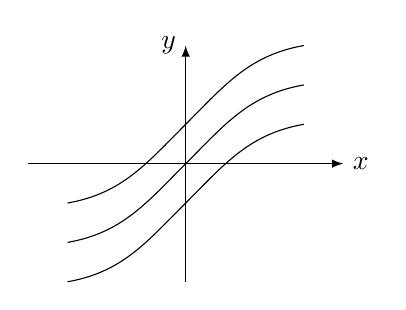
\begin{tikzpicture}
\pgfmathsetmacro{\l}{1.5}
\draw[-latex](-2,0)--(2,0)node[right]{$x$};
\draw[-latex](0,-1.5)--(0,1.5)node[left]{$y$};
\draw(0,0) to [out=-135,in=10]++(-\l,-1);
\draw(0,0) to [out=45,in=-170]++(\l,1);
\draw(0,0.5) to [out=-135,in=10]++(-\l,-1);
\draw(0,0.5) to [out=45,in=-170]++(\l,1);
\draw(0,-0.5) to [out=-135,in=10]++(-\l,-1);
\draw(0,-0.5) to [out=45,in=-170]++(\l,1);
\end{tikzpicture}
\caption{}
\end{subfigure}
\caption{منحنی کی عمومی صورت (مثال \حوالہ{مثال_تکمل_خاکہ})}
\label{شکل_مثال_تکمل_خاکہ_عمومی}
\end{figure}

پہلا تفرق مزید معلومات فراہم کرتا ہے:
\begin{align*}
\lim_{x\to \mp \infty}y'=\lim_{x\to \mp\infty}\frac{1}{x^2+1}=0
\end{align*}
یوں \عددی{x\to \mp \infty} پر منحنی افقی ہو گی۔

پانچواں قدم: \quad \ترچھا{مخصوص نقطے اور  منحنی حل۔} \quad
ہم جانتے ہیں کہ \عددی{x=0} پر منحنی کی ڈھلوان \عددی{1} ہے لہٰذا \عددی{y} محور کے کئی مقامات پر اکائی ڈھلوان کی (آپس میں متوازی) منحنیات کھینچتے ہیں شکل \حوالہ{شکل_مثال_تکمل_خاکہ_عمومی}-ج۔ 
\انتہا{مثال}
%=========================
\ابتدا{مثال}\شناخت{مثال_تکمل_مخصوص_خاکہ}
درج ذیل ابتدائی قیمت مسئلے کے حل کا خاکہ کھینچیں۔
\begin{align*}
y'&=\frac{1}{x^2+1}&&\text{\RL{تفرقی مساوات}}\\
y(0)&=0&&\text{\RL{ابتدائی معلومات}}
\end{align*}
حل:\quad
ہم نے مثال \حوالہ{مثال_تکمل_خاکہ} میں عمومی حل کا خاکہ کھینچا جس کو شکل \حوالہ{شکل_مثال_تکمل_خاکہ_عمومی}-ج میں دکھایا گیا ہے۔ان ترسیمات میں سے وہ ترسیم جو نقطہ \عددی{(0,0)} سے گزرتی ہے ابتدائی قیمت مسئلے کی درکار مخصوص حل ہے جس کو شکل \حوالہ{شکل_مثال_تکمل_مخصوص_خاکہ} میں دکھایا گیا ہے۔ 
\انتہا{مثال}
%=======================
\begin{figure}
\centering
\begin{tikzpicture}
\pgfmathsetmacro{\l}{1.5}
\draw[-latex](-2,0)--(2,0)node[right]{$x$};
\draw[-latex](0,-1.5)--(0,1.5)node[left]{$y$};
\draw(0,0)node[circ]{}node[below right]{$(0,0)$} to [out=-135,in=10]++(-\l,-1);
\draw(0,0) to [out=45,in=-170]++(\l,1);
\draw(-1,-1)--(1,1)node[pin=30:{ڈھلوان $=1$}]{};
\end{tikzpicture}
\caption{ابتدائی قیمت مسئلے کے مخصوص حل کا خاکہ (مثال \حوالہ{مثال_تکمل_مخصوص_خاکہ}) }
\label{شکل_مثال_تکمل_مخصوص_خاکہ}
\end{figure}

یہ ترکیب بالخصوص اس موقع پر بہت مددگار ثابت ہوتی ہے جب مساوات \عددی{\tfrac{\dif y}{\dif x}=f(x)} میں تفاعل \عددی{f(x)} کے الٹ تفرق کا بنیادی کلیہ نہیں پایا جاتا ہو۔ تفاعل \عددی{f(x)=\tfrac{1}{x^2+1}} کا الٹ تفرق پایا جاتا ہے، جس پر آگے  ایک باب میں غور کیا جائے گا، جبکہ تفاعل \عددی{g(x)=\sqrt{1+x^4}} کا الٹ تفرق نہیں پایا جاتا ہے۔ یوں تفرقی مساوات \عددی{\tfrac{\dif y}{\dif x}=\sqrt{1+x^4}} کو ہم ترسیمی یا اعدادی طریقہ سے حل کریں گے۔

\جزوحصہء{ریاضیاتی نمونہ کشی}
ریاضیاتی نمونہ کشی عموماً چار اقدام پر مبنی ہوتا ہے۔ ہم پہلے حقیقی دنیا میں کسی عمل (مثلاً گیند کا گرنا یا کھانسی کے دوران سانس کی نالی کا سکڑنا) کا مشاہدہ کرتے ہوئے اس کے اہم خصوصیات کو ظاہر کرنے والے ریاضی متغیرات کا نظام بناتے ہیں اور  معلومات کا ریاضی استعارہ کرتے ہیں۔  اس کے بعد متغیرات کے تعلقات کو  (عموماً) موجودہ ریاضی کی زبان میں لکھتے ہوئے نتائج اخذ کرتے ہیں۔ اس کے بعد ریاضیاتی حاصل نتائج کو زیر غور نظام پر لاگو کرتے ہیں۔ آخر میں ہم ریاضی نمونہ سے حاصل نتائج کا مشاہدے کے ساتھ موازنہ کرتے  ہوئے دیکھتے ہیں کہ آیا نمونہ پیش گوئی کر سکتا ہے۔ ہم یہ بھی دیکھتے ہیں کہ آیا نمونہ دیگر نظام پر قابل اطلاق ہو گا۔ بہترین نمونہ وہ  ہے جس کے نتائج مشاہدے کے عین مطابق ہوں، جو پیش گوئی کر سکے، جس کا استعمال وسیع اور آسان ہو۔ 

گیند کے گرنے کو مثال بناتے ہوئے مذکورہ بالا اقدام وضح کرتے ہیں۔ پہلے قدم پر ہم درج ذیل متغیرات اور مشاہدے اکٹھے کرتے ہیں۔\\
\موٹا{متغیرات:}\\
فاصلہ:\quad \عددی{s}\\
وقت:\quad \عددی{t}\\
\موٹا{ابتدائی قیمتیں:}\\
لمحہ \عددی{t=0} پر \عددی{s=0} اور \عددی{v=0} ہیں۔\\
\موٹا{فرض کیا گیا تعلق:}\quad \عددی{s=4.9t^2}\\
دوسرے قدم پر احصاء استعمال کرتے ہوئے درج ذیل ریاضی نتائج اخذ کرتے ہیں۔
\begin{align*}
v&=9.8t\\
a&=9.8
\end{align*}
تیسرے قدم پر نتائج کی تشریح کرتے ہوئے حقیقی دنیا کے لحاظ سے مفہوم بیان کرتے ہیں۔یوں لمحہ \عددی{t} پر رفتار \عددی{9.8t} میٹر فی سیکنڈ ہو گا جبکہ کسی بھی گرتے ہوئے جسم کی اسراع \عددی{\SI{9.8}{\meter\per\second\squared}} ہو گی۔ 

آخری قدم پر ہم آزادانہ گرنے والے جسم  کی لمحاتی رفتار اور اسراع ناپ کر تصدیق کرتے ہیں کہ ریاضی نمونہ درست نتائج کی پیش گوئی کر سکتا ہے۔

\جزوحصہء{نقل اترنا بذریعہ کمپیوٹر} 
کسی بھی نظام کو سمجھنے کی خاطر ہم مختلف حالات میں اس کا مشاہدہ کرتے ہیں۔ بعض پیچیدہ نظام کا  مشاہدہ کرنا ممکن نہیں ہوتا ہے۔ (مثلاً جب  مشاہدہ بہت مہنگا یا خطرناک ہو یا اس کے لئے بہت وقت درکار ہو۔) ایٹم بم یا سیلابی تباہی یا کہکشاں کا مشاہدہ  اس زمرے میں آتے ہیں۔ ان نظام پر غور کرنے کے لئے ہم ریاضی نمونہ کا سہارا لیتے ہیں۔ جہاں نظام کا حساب پیچیدہ یا بہت لمبا ہو وہاں کمپیوٹر کا استعمال سود مند ثابت ہوتا ہے۔ بلند عمارت، دریا پر پل یا برقیاتی ادوار بنانے سے پہلے ان کے نمونوں پر کمپیوٹر کی مدد سے غور کیا جاتا ہے۔ ہم کہتے ہیں کہ ہم کمپیوٹر پر عمل کا \اصطلاح{نقل اتارتے}\فرہنگ{نقل اتارنا}\حاشیہب{simulation}\فرہنگ{simulation} ہیں۔

\حصہء{سوالات}
\موٹا{ابتدائی قیمت مسائل}\\
\ابتدا{سوال}\شناخت{سوال_تکمل_ترسیمات_حل_الف}
درج ذیل ابتدائی قیمت مسئلے کا حل شکل \حوالہ{شکل_سوال_تکمل_ترسیمات_حل_الف} میں کون سی ترسیم پیش کرتا ہے؟ اپنے جواب کی وجہ پیش کریں۔
\begin{align*}
\frac{\dif y}{\dif x}&=2x\\
y(1)&=4
\end{align*}
جواب:\quad
(ب)
\انتہا{سوال}
%======================
\begin{figure}
\centering
\begin{subfigure}{0.30\textwidth}
\centering
\begin{tikzpicture}[font=\small]
\begin{axis}[clip=false,width=4cm, axis lines=middle,xlabel={$x$},ylabel={$y$},ymin=0,]
\addplot[domain=-1.5:1.5]{4*x^2};
\draw(axis cs:1,4)node[circ]{}node[right,font=\tiny]{$(1,4)$};
\end{axis}
\end{tikzpicture}
\caption{}
\end{subfigure}\hfill
\begin{subfigure}{0.30\textwidth}
\centering
\begin{tikzpicture}[font=\small]
\begin{axis}[clip=false,width=4cm, axis lines=middle,xlabel={$x$},ylabel={$y$},ymin=0,ytick={1,2,3,4}]
\addplot[domain=-1.5:1.5]{x^2+3};
\draw(axis cs:1,4)node[circ]{}node[right,font=\tiny]{$(1,4)$};
\end{axis}
\end{tikzpicture}
\caption{}
\end{subfigure}\hfill
\begin{subfigure}{0.30\textwidth}
\centering
\begin{tikzpicture}[font=\small]
\begin{axis}[clip=false,width=4cm, axis lines=middle,xlabel={$x$},ylabel={$y$},ytick={1,2,3,4}]
\addplot[domain=-1.5:1.5]{2*x+2};
\draw(axis cs:1,4)node[circ]{}node[right,font=\tiny]{$(1,4)$};
\end{axis}
\end{tikzpicture}
\caption{}
\end{subfigure}%
\caption{ترسیمات برائے سوال \حوالہ{سوال_تکمل_ترسیمات_حل_الف}}
\label{شکل_سوال_تکمل_ترسیمات_حل_الف}
\end{figure}

\ابتدا{سوال}\شناخت{سوال_تکمل_ترسیمات_حل_ب}
درج ذیل ابتدائی قیمت مسئلے کا حل شکل \حوالہ{شکل_سوال_تکمل_ترسیمات_حل_ب} میں کون سی ترسیم پیش کرتا ہے؟ اپنے جواب کی وجہ پیش کریں۔
\begin{align*}
\frac{\dif y}{\dif x}&=-x\\
y(-1)&=1
\end{align*}
جواب:\quad
(ب)
\انتہا{سوال}
%======================
\begin{figure}
\centering
\begin{subfigure}{0.30\textwidth}
\centering
\begin{tikzpicture}[font=\small]
\begin{axis}[clip=false,width=4cm, axis lines=middle,xlabel={$x$},ylabel={$y$},ymin=0,]
\addplot[domain=-1.5:1.5]{x^2};
\draw(axis cs:-1,1)node[circ]{}node[left,font=\tiny]{$(-1,1)$};
\end{axis}
\end{tikzpicture}
\caption{}
\end{subfigure}\hfill
\begin{subfigure}{0.30\textwidth}
\centering
\begin{tikzpicture}[font=\small]
\begin{axis}[clip=false,width=4cm, axis lines=middle,xlabel={$x$},ylabel={$y$},ymin=0,ymax=2,ytick={1}]
\addplot[domain=-1.5:1.5]{3/2-1/2*x^2};
\draw(axis cs:-1,1)node[circ]{}node[left,font=\tiny]{$(-1,1)$};
\end{axis}
\end{tikzpicture}
\caption{}
\end{subfigure}\hfill
\begin{subfigure}{0.30\textwidth}
\centering
\begin{tikzpicture}[font=\small]
\begin{axis}[clip=false,width=4cm, axis lines=middle,xlabel={$x$},ylabel={$y$},ytick={1,2,3,4}]
\addplot[domain=-1.5:1.5]{-x};
\draw(axis cs:-1,1)node[circ]{}node[below left,font=\tiny]{$(-1,1)$};
\end{axis}
\end{tikzpicture}
\caption{}
\end{subfigure}%
\caption{ترسیمات برائے سوال \حوالہ{سوال_تکمل_ترسیمات_حل_ب}}
\label{شکل_سوال_تکمل_ترسیمات_حل_ب}
\end{figure}

%=======================
سوال \حوالہ{سوال_تکمل_ابتدائی_قیمت_الف} تا سوال \حوالہ{سوال_تکمل_ابتدائی_قیمت_ب} میں دیے ابتدائی قیمت مسائل حل کریں۔ 

\ابتدا{سوال}\شناخت{سوال_تکمل_ابتدائی_قیمت_الف}
$\tfrac{\dif y}{\dif x}=2x-7,\quad y(2)=0$\\
جواب:\quad
$y=x^2-7x+10$
\انتہا{سوال}
%===================
\ابتدا{سوال}
$\tfrac{\dif y}{\dif x}=10-x,\quad y(0)=-1$
\انتہا{سوال}
%===================
\ابتدا{سوال}
$\tfrac{\dif y}{\dif x}=\tfrac{1}{x^2}+x,\,\, x>0,\quad y(2)=1$\\
جواب:\quad
$y=-\tfrac{1}{x}+\tfrac{x^2}{2}-\tfrac{1}{2}$
\انتہا{سوال}
%===================
\ابتدا{سوال}
$\tfrac{\dif y}{\dif x}=9x^2-4x+5,\quad y(-1)=0$
\انتہا{سوال}
%===================
\ابتدا{سوال}
$\tfrac{\dif y}{\dif x}=3x^{-2/3},\quad y(-1)=-5$\\
جواب:\quad
$y=9x^{1/3}+4$
\انتہا{سوال}
%===================
\ابتدا{سوال}
$\tfrac{\dif y}{\dif x}=\tfrac{1}{2\sqrt{x}},\quad y(4)=0$
\انتہا{سوال}
%===================
\ابتدا{سوال}
$\tfrac{\dif s}{\dif t}=1+\cos t,\quad s(0)=4$\\
جواب:\quad
$s=t+\sin t+4$
\انتہا{سوال}
%===================
\ابتدا{سوال}
$\tfrac{\dif s}{\dif t}=\cos t+\sin t,\quad s(\pi)=1$
\انتہا{سوال}
%===================
\ابتدا{سوال}
$\tfrac{\dif r}{\dif \theta}=-\pi\sin \pi \theta,\quad r(0)=0$\\
جواب:\quad
$r=\cos (\pi \theta)-1$
\انتہا{سوال}
%===================
\ابتدا{سوال}
$\tfrac{\dif  r}{\dif \theta}=\cos \pi\theta,\quad r(0)=1$
\انتہا{سوال}
%===================
\ابتدا{سوال}
$\tfrac{\dif v}{\dif t}=\tfrac{1}{2}\sec t\tan t,\quad v(0)=1$\\
جواب:\quad
$v=\tfrac{1}{2}\sec t+\tfrac{1}{2}$
\انتہا{سوال}
%===================
\ابتدا{سوال}
$\tfrac{\dif v}{\dif t}=8t+\csc^2 t,\quad v(\tfrac{\pi}{2})=-7$
\انتہا{سوال}
%===================
\ابتدا{سوال}
$\tfrac{\dif^{\,2}y}{\dif x^2}=2-6x,\quad y'(0)=4,\, y(0)=1$\\
جواب:\quad
$y=x^2-x^3+4x+1$
\انتہا{سوال}
%===================
\ابتدا{سوال}
$\tfrac{\dif^{\,2}y}{\dif x^2}=0,\quad y'(0)=2,\, y(0)=0$
\انتہا{سوال}
%===================
\ابتدا{سوال}
$\tfrac{\dif^{\,2}r}{\dif  t^2}=\tfrac{2}{t^3},\quad \left.\tfrac{\dif r}{\dif t}\right|_{t=1}=1,\,\, r(1)=1$\\
جواب:\quad
$r=\tfrac{1}{t}+2t-2$
\انتہا{سوال}
%===================
\ابتدا{سوال}
$\tfrac{\dif^{\,2}s}{\dif  t^2}=\tfrac{3t}{8},\quad \left.\tfrac{\dif s}{\dif t}\right|_{t=4}=3,\,\, s(4)=4$
\انتہا{سوال}
%===================
\ابتدا{سوال}
$\tfrac{\dif^{\,3}y}{\dif  x^3}=6,\,\, y''(0)=-8,\,\, y'(0)=0,\,\, y(0)=5$\\
جواب:\quad
$y=x^3-4x^2+5$
\انتہا{سوال}
%===================
\ابتدا{سوال}
$\tfrac{\dif^{\,3}\theta}{\dif  t^3}=0,\,\, \theta''(0)=-2,\,\, \theta'(0)=-\tfrac{1}{2},\,\, \theta(0)=\sqrt{2}$
\انتہا{سوال}
%===================
\ابتدا{سوال}
$y^{(4)}=-\sin t+\cos t,\,\, y'''(0)=7,\,\, y''(0)=y'(0)=-1,\,\, y(0)=0$\\
جواب:\quad
$y=-\sin t+\cos t+t^3-1$
\انتہا{سوال}
%===================
\ابتدا{سوال}\شناخت{سوال_تکمل_ابتدائی_قیمت_ب}
$y^{(4)}=-\cos x+8\sin 2x,\,\, y'''(0)=0, \,\, y''(0)=y'(0)=1,\,\, y(0)=3$
\انتہا{سوال}
%===================
\موٹا{رفتار سے مقام معلوم کرنا}\\
سوال \حوالہ{سوال_تکمل_رفتار_سے_مقام_الف} تا سوال \حوالہ{سوال_تکمل_رفتار_سے_مقام_ب} میں رفتار \عددی{v=\tfrac{\dif s}{\dif t}} اور ابتدائی مقام دیے گیے ہیں۔ لمحہ \عددی{t} پر جسم کا مقام تلاش کریں۔

\ابتدا{سوال}\شناخت{سوال_تکمل_رفتار_سے_مقام_الف}
$v=9.8 t+5,\quad s(0)=10$\\
جواب:\quad
$s=4.9t^2+5t+10$
\انتہا{سوال}
%=======================
\ابتدا{سوال}
$v=32 t-2,\quad s(1/2)=4$
\انتہا{سوال}
%=======================
\ابتدا{سوال}
$v=\sin \pi t,\quad s(0)=0$\\
جواب:\quad
$s=\tfrac{1-\cos (\pi t)}{\pi}$
\انتہا{سوال}
%=======================
\ابتدا{سوال}\شناخت{سوال_تکمل_رفتار_سے_مقام_ب}
$v=\tfrac{2}{\pi}\cos \tfrac{2t}{\pi},\quad s(\pi^2)=1$
\انتہا{سوال}
%=======================
\موٹا{اسراع سے مقام کی تلاش}\\
سوال \حوالہ{سوال_تکمل_اسراع_سے_مقام_الف} تا سوال \حوالہ{سوال_تکمل_اسراع_سے_مقام_ب} میں اسراع \عددی{a=\tfrac{\dif^2 s}{\dif t^2}}، ابتدائی رفتار  اور ابتدائی مقام دیے گئے ہیں۔لمحہ \عددی{t} پر جسم کا مقام تلاش کریں۔

\ابتدا{سوال}\شناخت{سوال_تکمل_اسراع_سے_مقام_الف}
$a=32,\quad v(0)=20,\quad s(0)=5$\\
جواب:\quad
$s=16t^2+20t+5$
\انتہا{سوال}
%=========================
\ابتدا{سوال}
$a=9.8,\quad v(0)=-3,\quad s(0)=0$
\انتہا{سوال}
%=========================
\ابتدا{سوال}
$a=-4\sin 2t,\quad v(0)=2,\quad s(0)=-3$\\
جواب:\quad
$s=\sin (2t)-3$
\انتہا{سوال}
%=========================
\ابتدا{سوال}\شناخت{سوال_تکمل_اسراع_سے_مقام_ب}
$a=\tfrac{9}{\pi^2}\cos\tfrac{3t}{\pi},\quad v(0)=0,\quad s(0)=-1$
\انتہا{سوال}
%=========================
\موٹا{ترسیم کا حصول}\\
\ابتدا{سوال}
ایسی ترسیم \عددی{y=f(x)} تلاش کریں جو نقطہ \عددی{(9,4)} سے گزرتی ہو اور جس کی ڈھلوان \عددی{3\sqrt{x}} ہو۔ \\
جواب:\quad
$y=2x^{3/2}-50$
\انتہا{سوال}
%===================
\ابتدا{سوال}
منحنی \عددی{y=f(x)} نقطہ \عددی{(0,1)} سے گزرتی ہے جہاں اس کا مماس افقی ہے۔یہ ترسیم \عددی{\tfrac{\dif^{\,2}y}{\dif x^2}=6x} کو مطمئن کرتی ہے۔ اس ترسیم کو تلاش کریں۔
\انتہا{سوال}
%================
\موٹا{منحنیات حل (تکملی منحنیات)}\\
سوال \حوالہ{سوال_تکمل_ترسیم_کا_حصول_الف} تا سوال \حوالہ{سوال_تکمل_ترسیم_کا_حصول_د} میں منحنی حل دکھائے گئے ہیں۔ دیے نقطے پر منحنی کی مساوات تلاش کریں۔
\begin{figure}
\centering
\begin{minipage}{0.22\textwidth}
\centering
\begin{tikzpicture}[font=\small,declare function={f(\x)=\x-(\x^2)^(2/3);}]
\begin{axis}[clip=false,width=4cm,axis lines=middle,xlabel={$x$},ylabel={$y$},xlabel style={at={(current axis.right of origin)},anchor=west},ylabel style={at={(current axis.above origin)},anchor=south},ymax=1.5,xmax=2.25,xtick={\empty},ytick={\empty}]
\addplot[domain=-0.5:2]{f(x)};
\addplot[domain=-0.5:2]{f(x)-0.5};
\addplot[domain=-0.5:2]{f(x)-1};
\addplot[domain=-0.5:2]{f(x)-1.5};
\addplot[domain=-0.5:2]{f(x)+0.5};
\addplot[domain=-0.5:2]{f(x)+1};
\draw(axis cs:1,0.5)node[right,fill=white,font=\tiny]{$(1,0.5)$}node[circ]{};
\draw(0.24,1.35)node[right,font=\tiny]{$\frac{\dif y}{\dif x}=1-\frac{4}{3}x^{1/3}$};
\end{axis}
\end{tikzpicture}
\caption{منحنیات برائے سوال \حوالہ{سوال_تکمل_ترسیم_کا_حصول_الف}}
\label{شکل_سوال_تکمل_ترسیم_کا_حصول_الف}
\end{minipage}\hfill
\begin{minipage}{0.22\textwidth}
\centering
\begin{tikzpicture}[font=\small,declare function={f(\x)=1/2*\x^2-\x;}]
\begin{axis}[width=4cm,axis lines=middle,xlabel={$x$},ylabel={$y$},xlabel style={at={(current axis.right of origin)},anchor=west},ylabel style={at={(current axis.above origin)},anchor=south},ymax=1.5,xmax=2.25,xtick={\empty},ytick={\empty}]
\addplot[domain=-1.5:2]{f(x)};
\addplot[domain=-1.5:2]{f(x)-0.5};
\addplot[domain=-1.5:2]{f(x)-1};
\addplot[domain=-1.5:2]{f(x)-1.5};
\addplot[domain=-1.5:2]{f(x)+0.5};
\addplot[domain=-1.5:2]{f(x)+1};
\draw(axis cs:-1,1)node[above,fill=white,font=\tiny]{$(-1,1)$}node[circ]{};
\draw(0.24,1.2)node[right,font=\tiny]{$\frac{\dif y}{\dif x}=x-1$};
\end{axis}
\end{tikzpicture}
\caption{منحنیات برائے سوال \حوالہ{سوال_تکمل_ترسیم_کا_حصول_ب}}
\label{شکل_سوال_تکمل_ترسیم_کا_حصول_ب}
\end{minipage}\hfill
\begin{minipage}{0.22\textwidth}
\centering
\begin{tikzpicture}[font=\small,declare function={f(\x)=-cos(deg(\x))-sin(deg(\x));}]
\begin{axis}[clip=false,width=4cm,axis lines=middle,xlabel={$x$},ylabel={$y$},xlabel style={at={(current axis.right of origin)},anchor=west},ylabel style={at={(current axis.above origin)},anchor=south},ymax=1.5,xmax=5.5,xtick={\empty},ytick={\empty}]
\addplot[domain=-4:5]{f(x)};
\addplot[domain=-4:5]{f(x)-0.5};
\addplot[domain=-4:5]{f(x)-1};
\addplot[domain=-4:5]{f(x)-1.5};
\addplot[domain=-4:5]{f(x)-2};
\addplot[domain=-3:5]{f(x)-2.5};
\addplot[domain=-4.1:5]{f(x)+0.5};
\draw(axis cs:-3.142,-1)node[below,fill=white,font=\tiny]{$(-\pi,-1)$}node[circ]{};
\draw(0.24,1.35)node[right,fill=white,font=\tiny]{$\frac{\dif y}{\dif x}=\sin x-\cos x$};
\end{axis}
\end{tikzpicture}
\caption{منحنیات برائے سوال \حوالہ{سوال_تکمل_ترسیم_کا_حصول_ج}}
\label{شکل_سوال_تکمل_ترسیم_کا_حصول_ج}
\end{minipage}\hfill
\begin{minipage}{0.22\textwidth}
\centering
\begin{tikzpicture}[font=\small,declare function={f(\x)=sqrt(\x)+cos(deg(\x));}]
\begin{axis}[clip=false,width=4cm,axis lines=middle,xlabel={$x$},ylabel={$y$},xlabel style={at={(current axis.right of origin)},anchor=west},ylabel style={at={(current axis.above origin)},anchor=south},ymax=3.5,xmax=3.5,xtick={\empty},ytick={\empty}]
\addplot[domain=0:3]{f(x)};
\addplot[domain=0:3]{f(x)-0.5};
\addplot[domain=0:3]{f(x)-1};
\addplot[domain=0:3]{f(x)+0.5};
\addplot[domain=0:3]{f(x)+1};
\draw(axis cs:1,2)node[below,fill=white,font=\tiny]{$(1,2)$}node[circ]{};
\draw(0.24,3.35)node[right,fill=white,font=\tiny]{$\frac{\dif y}{\dif x}=\tfrac{1}{2\sqrt {x}}+\pi\sin \pi x$};
\end{axis}
\end{tikzpicture}
\caption{منحنیات برائے سوال \حوالہ{سوال_تکمل_ترسیم_کا_حصول_د}}
\label{شکل_سوال_تکمل_ترسیم_کا_حصول_د}
\end{minipage}
\end{figure}

\ابتدا{سوال}\شناخت{سوال_تکمل_ترسیم_کا_حصول_الف}
ترسیمات کو شکل \حوالہ{سوال_تکمل_ترسیم_کا_حصول_الف} میں دکھایا گیا ہے۔\\
جواب:\quad
$y=x-x^{4/3}+\tfrac{1}{2}$
\انتہا{سوال}
%======================
\ابتدا{سوال}\شناخت{سوال_تکمل_ترسیم_کا_حصول_ب}
ترسیمات کو شکل \حوالہ{سوال_تکمل_ترسیم_کا_حصول_ب} میں دکھایا گیا ہے۔
\انتہا{سوال}
%======================
\ابتدا{سوال}\شناخت{سوال_تکمل_ترسیم_کا_حصول_ج}
ترسیمات کو شکل \حوالہ{سوال_تکمل_ترسیم_کا_حصول_ج} میں دکھایا گیا ہے۔\\
جواب:\quad
$y=-\sin x-\cos x-2$
\انتہا{سوال}
%======================
\ابتدا{سوال}\شناخت{سوال_تکمل_ترسیم_کا_حصول_د}
ترسیمات کو شکل \حوالہ{سوال_تکمل_ترسیم_کا_حصول_د} میں دکھایا گیا ہے۔
\انتہا{سوال}
%======================
تفرقی مساوات کے حل کا خاکہ کھینچنا مثال \حوالہ{مثال_تکمل_خاکہ} میں سکھایا گیا۔اس ترکیب کو استعمال کرتے ہوئے سوال \حوالہ{سوال_تکمل_خاکہ_الف} تا سوال \حوالہ{سوال_تکمل_خاکہ_ب} میں دیے گئے تفرقی مساوات کے حل کے خاکے بنائیں۔

\ابتدا{سوال}\شناخت{سوال_تکمل_خاکہ_الف}
$\tfrac{\dif y}{\dif x}=2x$\\
جواب:\quad
شکل \حوالہ{شکل_سوال_تکمل_خاکہ_الف}
\انتہا{سوال}
%==========================
\ابتدا{سوال}
$\tfrac{\dif y}{\dif x}=-2x+2$
\انتہا{سوال}
%=========================
\ابتدا{سوال}
$\tfrac{\dif y}{\dif x}=1-3x^2$\\
جواب:\quad
شکل \حوالہ{شکل_سوال_تکمل_خاکہ_پ}
\انتہا{سوال}
%=========================
\ابتدا{سوال}\شناخت{سوال_تکمل_خاکہ_ب}
$\tfrac{\dif y}{\dif x}=x^2$
\انتہا{سوال}
%=========================
\begin{figure}
\centering
\begin{minipage}{0.22\textwidth}
\centering
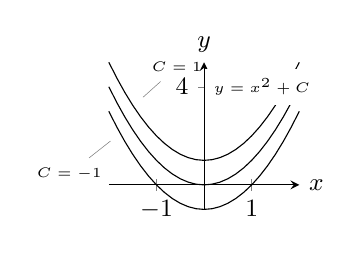
\begin{tikzpicture}[font=\small,declare function={f(\x)=\x^2;}]
\begin{axis}[clip=false,width=4cm, axis lines=middle, xlabel={$x$},ylabel={$y$},xlabel style={at={(current axis.right of origin)},anchor=west},ylabel style={at={(current axis.above origin)},anchor=south},xtick={-1,1},ytick={4}]
\addplot[domain=-2:2]{f(x)+0};
\addplot[domain=-2:2]{f(x)-1}node[pos=0.1,pin={[pin distance=0.2cm, font=\tiny]-110:{$C=-1$}}]{};
\addplot[domain=-2:2]{f(x)+1}node[pos=0.2,pin={[pin distance=0.2cm,font=\tiny]70:{$C=1$}}]{};
\draw(axis cs:0,4)node[right,fill=white,font=\tiny]{$y=x^2+C$};
\end{axis}
\end{tikzpicture}
\caption{}
\label{شکل_سوال_تکمل_خاکہ_الف}
\end{minipage}\hfill
\begin{minipage}{0.22\textwidth}
\centering
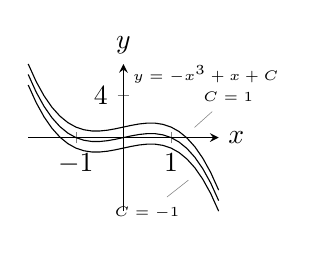
\begin{tikzpicture}[declare function={f(\x)=-\x^3+\x;}]
\begin{axis}[clip=false,width=4cm, axis lines=middle, xlabel={$x$},ylabel={$y$},xlabel style={at={(current axis.right of origin)},anchor=west},ylabel style={at={(current axis.above origin)},anchor=south},xtick={-1,1},ytick={4}]
\addplot[domain=-2:2]{f(x)+0};
\addplot[domain=-2:2]{f(x)-1}node[pos=0.75,pin={[pin distance=0.2cm,font=\tiny]-110:{$C=-1$}}]{};
\addplot[domain=-2:2]{f(x)+1}node[pos=0.65,pin={[pin distance=0.2cm,font=\tiny]70:{$C=1$}}]{};
\draw(axis cs:0,6)node[right,font=\tiny]{$y=-x^3+x+C$};
\end{axis}
\end{tikzpicture}
\caption{}
\label{شکل_سوال_تکمل_خاکہ_پ}
\end{minipage}\hfill
\begin{minipage}{0.22\textwidth}
\centering
\begin{tikzpicture}[font=\small]
\draw[-latex](-1.1,0)--(1.1,0)node[right]{$x$};
\draw[-latex](0,-1.1)--(0,1.1)node[above]{$y$};
\draw(-1,-1) to [out=90,in=-90](1,1);
\draw(0,0)node[pin=135:{ڈھلوان $=1$}]{};
\foreach \x in {-1,1}{\draw(\x,0)node[below]{$\x$}--++(0,0.1);}
\foreach \y in {-1,1}{\draw(0,\y)node[left]{$\y$}--++(0.1,0);}
\end{tikzpicture}
\caption{}
\label{شکل_سوال_تکمل_خاکہ_تیار_الف}
\end{minipage}\hfill
\begin{minipage}{0.22\textwidth}
\centering
\begin{tikzpicture}[font=\small]
\draw[-latex](-1.1,0)--(1.1,0)node[right]{$x$};
\draw[-latex](0,0)--(0,2.2)node[above]{$y$};
\draw(0,1)node[pin=45:{ڈھلوان $=0$}]{};
\foreach \y in {1}{\draw(0,\y)node[left]{$\y$}--++(0.1,0);}
\draw(-1,1.5) to [out=-45,in=135](1,0.5);
\end{tikzpicture}
\caption{}
\label{شکل_سوال_تکمل_خاکہ_تیار_پ}
\end{minipage}
\end{figure}
سوال \حوالہ{سوال_تکمل_خاکہ_تیار_الف} تا سوال \حوالہ{سوال_تکمل_خاکہ_تیار_ب} میں دیے گئے تفرقی مساوات کے حل کا خاکہ مثال \حوالہ{مثال_تکمل_خاکہ} اور مثال \حوالہ{مثال_تکمل_مخصوص_خاکہ} کی طرح بنائیں۔

\ابتدا{سوال}\شناخت{سوال_تکمل_خاکہ_تیار_الف}
$\tfrac{\dif y}{\dif x}=\tfrac{1}{\sqrt{1-x^2}},\quad -1<x<1;\quad y(0)=0$\\
جواب:\quad
شکل \حوالہ{شکل_سوال_تکمل_خاکہ_تیار_الف}
\انتہا{سوال}
%====================
\ابتدا{سوال}
$\tfrac{\dif y}{\dif x}=\sqrt{1+x^4}, \quad y(0)=1$
\انتہا{سوال}
%====================
\ابتدا{سوال}
$\tfrac{\dif y}{\dif x}=\tfrac{1}{x^2+1}-1,\quad y(0)=1$\\
جواب:\quad
شکل \حوالہ{شکل_سوال_تکمل_خاکہ_تیار_پ}
\انتہا{سوال}
%====================
\ابتدا{سوال}\شناخت{سوال_تکمل_خاکہ_تیار_ب}
$\tfrac{\dif y}{\dif x}=\tfrac{x}{x^2+1},\quad y(0)=0$
\انتہا{سوال}
%====================
\موٹا{عملی استعمال}\\
\ابتدا{سوال}
چاند پر ثقلی اسراع \عددی{\SI{1.6}{\meter\per\second\squared}} ہے۔ ایک پتھر کو چاند پر گہرے شگاف میں گرایا جاتا ہے۔اس کی رفتار اس لمحہ پر کیا ہو گی جب یہ \عددی{30} سیکنڈ بعد شگاف کی تہہ تک پہنچتا ہے؟\\
جواب:\quad
$\SI{48}{\meter\per\second}$
\انتہا{سوال}
%====================
\ابتدا{سوال}
ایک راکٹ سطح زمین سے سیدھا اوپر رخ \عددی{\SI{20}{\meter\per\second\squared}} کی اسراع سے اڑتا ہے۔ ایک منٹ بعد اس کی رفتار کیا ہو گی؟
\انتہا{سوال}
%====================
\ابتدا{سوال}
\عددی{\SI{10}{\meter}} بلندی سے پانی میں کھودا جاتا ہے۔ پانی میں داخل ہوتے ہوئے لمحے پر آپ کی رفتار کیا ہو گی؟ \عددی{g=\SI{9.8}{\meter\per\second\squared}} لیں۔ \\
جواب:\quad
$\SI{14}{\meter\per\second}$
\انتہا{سوال}
%========================
\ابتدا{سوال}
مریخ پر سطح کے نزدیک ثقلی اسراع \عددی{\SI{3.72}{\meter\per\second\squared}} ہے۔ایک راکٹ جس کو مریخ کی سطح سے \عددی{\SI{93}{\meter\per\second}} کی ابتدائی رفتار سے سیدھا اوپر پھینکا جائے کس بلندی تک پہنچے گا؟ 
\انتہا{سوال}
%=======================
\ابتدا{سوال}
آپ اسلام آباد تا لاہور موٹروے پر \عددی{\SI{100}{\kilo\meter\per\hour}} کی رفتار سے صفر کر رہے  ہیں جب آپ کو سامنے ایک حادثہ نظر آتا ہے۔ آپ یکدم گاڑی کو روکنے کی کوشش کرتے ہیں۔ گاڑی \عددی{\SI{75}{\meter}} میں مکمل رک جاتی ہے۔ رکنے کی اسراع تلاش کریں۔ اس کا جواب حاصل کرنے کی خاطر درج ذیل  کرنا ہو گا۔\\
\موٹا{پہلا قدم:}\quad درج ذیل ابتدائی قیمت مسئلہ حل کریں۔
\begin{align*}
\frac{\dif^{\,2}s}{\dif t^2}&=-k&&\text{\RL{$\,k\,$ مستقل}}\\
\frac{\dif s}{\dif t}(0)&=100,\quad s(0)=0&&\text{\RL{ابتدائی معلومات}}
\end{align*}
\موٹا{دوسرا قدم:}\quad \عددی{t} کی وہ قیمت تلاش کریں جس پر \عددی{\tfrac{\dif s}{\dif t}=0} حاصل ہو گا۔(آپ کے جواب میں \عددی{k} پایا جائے گا۔)\\
\موٹا{تیسرا قدم:}\quad \عددی{k} کی وہ قیمت تلاش کریں جس پر \عددی{s=75} حاصل ہوتا ہے۔\\
جواب:\quad
$t=\tfrac{100}{k},\,\,k=\tfrac{200}{3}\,\si{\kilo\meter\per\hour\squared}$
\انتہا{سوال}
%===========================
\ابتدا{سوال}
موٹر سائکل پر با حفاظت صفر کے لئے لازمی ہے کہ آپ \عددی{\SI{50}{\kilo\meter\per\hour}} کی رفتار سے  \عددی{\SI{14}{\meter}} میں رک سکیں۔ ایسا کرنے کے لئے کتنی اسراع درکار ہو گی؟ 
\انتہا{سوال}
%===========================
\ابتدا{سوال}
ایک ذرہ محوری لکیر پر \عددی{\tfrac{\dif^2s}{\dif t^2}=15\sqrt{t}-\tfrac{3}{\sqrt{t}}} اسراع سے حرکت کرتا ہے۔ لمحہ \عددی{t=1} پر \عددی{s=0} اور \عددی{\tfrac{\dif s}{\dif t}=4} ہیں۔ لمحہ \عددی{t} پر \عددی{v=\tfrac{\dif s}{\dif t}} اور \عددی{s} تلاش کریں۔ \\
جواب:\quad
$v=10t^{3/2}-6t^{1/2},\,\, s=4t^{5/2}-4t^{3/2}$
\انتہا{سوال}
%=======================
\ابتدا{سوال}
چاند پر اپالو-15 پرواز کے داؤد سکاٹ نے پر اور  ہتھوڑے کو تقریباً \عددی{\SI{1.25}{\meter}} بلندی سے ایک ساتھ گرنے دیا۔ چاند پر ہوا کی غیر موجودگی کی بنا دونوں کے گرنے کی رفتار یکساں تھی۔ بتائیں گرنے کا دورانیہ کتنا تھا؟ گرنے کا دورانیہ دریافت کرنے کے لئے درج ذیل ابتدائی قیمت مسئلہ حل کرتے ہوئے تفاعل \عددی{s} تلاش کریں جس کا آزاد متغیر \عددی{t} ہو۔ اس کے بعد \عددی{t} کی وہ قیمت تلاش کریں جو \عددی{s=0} دے۔
\begin{align*}
\frac{\dif^{\,2}s}{\dif t^2}&=\SI{-1.6}{\meter\per\second\squared}&&\text{\RL{تفرقی مساوات}}\\
\frac{\dif s}{\dif t}(0)&=0,\,\, s(0)=1.25&&\text{\RL{ابتدائی معلومات}}
\end{align*}
\انتہا{سوال}
%============================
\ابتدا{سوال}
محددی لکیر پر مستقل اسراع \عددی{a} سے حرکت کرتے ہوئے جسم کے مقام \عددی{s} کی معیاری مساوات درج ذیل ہے
\begin{align}\label{مساوات_تکمل_گرتا_ہوا_جسم_الف}
s=\frac{1}{2}at^2+v_0t+s_0
\end{align}
جہاں لمحہ \عددی{t=0}پر جسم کی رفتار \عددی{v_0} اور مقام \عددی{s_0} ہیں۔درج ذیل ابتدائی قیمت مسئلہ حل کرتے ہوئے اس مساوات کو اخذ کریں۔
\begin{align*}
\frac{\dif^{\,2}s}{\dif t^2}&=a&&\text{\RL{تفرقی مساوات}}\\
\frac{\dif s}{\dif t}(0)&=v_0,\,\, s(0)=s_0&&\text{\RL{ابتدائی معلومات}}
\end{align*}
\انتہا{سوال}
%=====================
\ابتدا{سوال}
سیارہ کی سطح کے نزدیک آزادی کے ساتھ گرتے ہوئے جسم کا مقام درج ذیل مساوات دیتی ہے
\begin{align}\label{مساوات_تکمل_گرتا_ہوا_جسم_ب}
s=-\frac{1}{2}gt^2+v_0t+s_0
\end{align}
جہاں ثقلی اسراع \عددی{a}، سطح سیارہ سے جسم کی ابتدائی بلندی \عددی{s_0} اور جسم کی ابتدائی رفتار \عددی{v_0} ہے۔ چونکہ اسراع نیچے رخ (بلندی \عددی{s} کے الٹ) ہے لہٰذا مساوات میں منفی کی علامت پائی جاتی ہے۔ اگر لمحہ \عددی{t=0} پر جسم کی رفتار اوپر رخ ہو تب \عددی{v_0} مثبت ہو گا اور اگر اس کا رخ نیچے کو ہو تب \عددی{v_0} منفی ہو گا۔ 

مساوات \حوالہ{مساوات_تکمل_گرتا_ہوا_جسم_الف} استعمال کیے بغیر آپ مساوات \حوالہ{مساوات_تکمل_گرتا_ہوا_جسم_ب} ایک ابتدائی قیمت مسئلہ حل کرتے ہوئے حاصل کر سکتے ہیں۔ یہ ابتدائی قیمت مسئلہ کیا ہو گا؟ اس مسئلے کو حل کرتے ہوئے مساوات \حوالہ{مساوات_تکمل_گرتا_ہوا_جسم_ب} کو حاصل کریں۔
\انتہا{سوال}
%=========================
\موٹا{نظریہ اور مثالیں}\\
\ابتدا{سوال}\شناخت{سوال_تکمل_رفتار_سے_ہٹاو}\ترچھا{رفتار کی الٹ تفرق سے ہٹاو کا تعین۔}\\
\begin{enumerate}[a.]
\item
فرض کریں محور \عددی{s} پر ایک جسم کی رفتار \عددی{\tfrac{\dif s}{\dif t}=v=9.8t-3} ہے۔
\begin{enumerate}[1.]
\item
اگر \عددی{t=0} پر \عددی{s=5} ہو تب \عددی{t=1} تا \عددی{t=3} جسم کا ہٹاو تلاش کریں۔
\item
اگر \عددی{t=0} پر \عددی{s=-2} ہو تب \عددی{t=1} تا \عددی{t=3} جسم کا ہٹاو تلاش کریں۔
\item
اگر \عددی{t=0} پر \عددی{s=s_0} ہو تب \عددی{t=1} تا \عددی{t=3} جسم کا ہٹاو تلاش کریں۔
\end{enumerate}
\item
فرض کریں محددی لکیر پر ایک جسم کا مقام \عددی{s} متغیر \عددی{t} کا قابل تفرق تفاعل ہے۔کیا یہ درست ہے کہ \عددی{\tfrac{\dif s}{\dif t}} کا الٹ تفرق جانتے ہوئے دورانیہ \عددی{t=a} تا \عددی{t=b} کے لئے آپ جسم کا ہٹاو جان سکتے ہیں اگرچہ ان دونوں لمحات پر آپ کو جسم کا ہٹاو معلوم نہیں ہے؟ اپنے جوان کی وجہ پیش کریں۔  
\end{enumerate}
جواب:\quad
(الف) \عددی{\SI{33.2}{\meter}}، \عددی{\SI{33.2}{\meter}}، \عددی{\SI{33.2}{\meter}} ، (ب)  درست
\انتہا{سوال}
%=====================
\ابتدا{سوال}\ترچھا{یکتائی حل}\\
اگر قابل تفرق تفاعل \عددی{y=F(x)} اور \عددی{y=G(x)} وقفہ \عددی{I} پر درج ذیل ابتدائی قیمت مسئلے کے حل ہوں تب کیا \عددی{I} میں ہر \عددی{x} کے لئے \عددی{F(x)=G(x)} ہو گا؟ اپنے جواب کی وجہ پیش کریں۔
\انتہا{سوال}
%=======================

\حصہ{تکمل بذریعہ ترکیب بدل۔ زنجیری قاعدہ کا الٹ اطلاق}
بعض اوقات انجناے تکمل میں  متغیرات کی تبدیلی سے جانا پہچانا تکمل حاصل ہوتا ہے۔ تکمل کے اس طریقہ کو ترکیب بدل کہتے ہیں۔  تکمل کے حصول کا یہ ایک اہم ترین طریقہ ہے۔ آئیں اس ترکیب کو سمجھتے ہیں۔

\جزوحصہء{عمومی طاقتی قاعدہ کی تکملی صورت}
جب \عددی{u}  متغیر \عددی{x} کا قابل تفرق تفاعل ہو اور \عددی{n} ناطق عدد ہو جس کی قیمت \عددی{-1} نہ ہو تب زنجیری قاعدہ کے تحت درج ذیل ہو گا۔
\begin{align*}
\frac{\dif}{\dif x}\big(\frac{u^{n+1}}{n+1}\big)=u^n\frac{\dif u}{\dif x}
\end{align*}
اس مساوات کو ایک دوسری نقطہ نظر سے دیکھتے ہوئے ہم کہہ سکتے ہیں کہ تفاعل \عددی{u^n\tfrac{\dif u}{\dif x}} کا ایک الٹ تفرق \عددی{\tfrac{u^{n+1}}{n+1}} ہے لہٰذا درج ذیل لکھا جا سکتا ہے۔
\begin{align*}
\int \big(u^n\tfrac{\dif u}{\dif x}\big)\dif x=\frac{u^{n+1}}{n+1}+C
\end{align*}
اس مساوات کے بائیں ہاتھ کو عموماً درج ذیل سادہ تفرقی روپ میں لکھا جاتا ہے
\begin{align*}
\int u^n\dif u
\end{align*}
جہاں دونوں \عددی{\dif x} کو آپس میں کاٹا گیا ہے۔درج بالا دو مساوات کو ملا کر درج ذیل ملتا ہے
\begin{align}\label{مساوات_تکمل_پہلا_کلیہ}
\int u^n\dif u=\frac{u^{n+1}}{n+1}+C,&&(n\ne -1, \,\, \text{\RL{$n$ ناطق}})
\end{align}
جہاں \عددی{u} قابل تفرق تفاعل ہے اور \عددی{\dif u} اس کا تفرق ہے۔

مساوات \حوالہ{مساوات_تکمل_پہلا_کلیہ} حاصل کرتے ہوئے ہم فرض کرتے ہیں کہ \عددی{u} متغیر \عددی{x} کا قابل تفرق تفاعل ہے، اگرچہ یہ متغیر اس کلیہ میں نہیں پایا جاتا ہے اور اس کی علامت اہم نہیں ہے۔ ہم اس متغیر کو کسی بھی علامت مثلاً \عددی{\theta}، \عددی{t}، \عددی{y}وغیرہ سے ظاہر کر سکتے تھے۔ مساوات \حوالہ{مساوات_تکمل_پہلا_کلیہ} کہتی ہے کہ جب بھی ہم کسی تکمل کو درج ذیل روپ میں لکھ سکیں
\begin{align*}
\int u^n\dif u,\quad \quad (n\ne -1)
\end{align*}
جہاں \عددی{u} قابل تفرق تفاعل ہو اور \عددی{\dif u} اس کا تفرق ہو تب اس کا حل \عددی{\tfrac{u^{n+1}}{n+1}+C} ہو گا۔

\ابتدا{مثال}
درج ذیل تکمل حل کریں۔
\begin{align*}
\int(x+2)^5\dif x
\end{align*}
حل:\quad
ہم اس تکمل کو درج ذیل روپ میں لکھتے ہیں۔
\begin{align*}
\int u^n\dif u
\end{align*}
ایسا کرنے کی خاطر ہم \عددی{u=x+2} لیتے ہیں لہٰذا \عددی{\dif u=\dif x} ہو گا۔یوں درج ذیل حاصل ہو گا۔
\begin{align*}
\int (x+2)^5\dif x&=\int u^5\dif u&&u=x+2,\,\,\dif u=\dif x\\
&=\frac{u^6}{6}+C&& \text{\RL{مساوات \حوالہ{مساوات_تکمل_پہلا_کلیہ} میں $n=5$}}\\
&=\frac{(x+2)^6}{6}+C&&\text{\RL{واپس $u=x+2$ پر کریں}}
\end{align*}
\انتہا{مثال}
%==============
\ابتدا{مثال}
\عددی{u=x^2+2x-3} لیتے ہوئے \عددی{\dif u=2x\dif x+2\dif=2(x+1)\dif x} اور \عددی{\tfrac{1}{2}\dif u=(x+1)\dif x} ہو گا۔ یوں تکمل
\begin{align*}
\int (x^2+2x-3)^2(x+1)\dif x
\end{align*}
کو ترکیب بدل سے  حل کیا جا سکتا ہے:
\begin{align*}
\int (x^2+2x-3)^2(x+1)\dif x&=\int u^2\cdot \frac{1}{2}\dif u\\
&=\frac{1}{2}\int u^2\dif u\\
&=\frac{1}{2}\frac{u^3}{3}+C=\frac{1}{6}u^3+C&&\text{\RL{$u$ کے لحاظ سے تکمل}}\\
&=\frac{1}{6}(x^2+2x-3)+C&&\text{\RL{$u$ بدلیں}}
\end{align*}
آخری قدم پر \عددی{u} کی قیمت واپس پر کی گئی ہے۔
\انتہا{مثال}
%===========================
\ابتدا{مثال}
\begin{align*}
\int\sin^4t\cos t\dif t&=\int u^4\dif u&&u=\sin t,\,\, \dif u=\cos t\dif t\\
&=\frac{u^5}{5}+C&&\text{\RL{$u$ کے لحاظ سے تکمل}}\\
&=\frac{\sin^5t}{5}+C&&\text{\RL{$u$ بدلیں}}
\end{align*}
\انتہا{مثال}
%========================

ترکیب بدل کی کامیابی اس بات پر منحصر ہے کہ ہم ایسا بدل تلاش کر سکیں جو مشکل تکمل کو جانے پہچانے تکمل میں تبدیل کرتا ہو۔بعض اوقات پہلے بدل کے بعد دوسرا اور تیسرا بدل بھی درکار ہوتا ہے یا ہم کوئی دوسرا بدل استعمال کرنے کی کوشش کر سکتے ہیں۔ بعض اوقات کئی مختلف بدل قابل استعمال ہوں گے (اگلا مثال)۔

\ابتدا{مثال}
درج ذیل تکمل حل کریں۔
\begin{align*}
\int\frac{2z\dif z}{\sqrt[3]{z^2+1}}
\end{align*}
حل:\quad
ہم متکمل کے مشکل ترین حصے کی سادہ صورت تلاش کرنے کی غرض سے \عددی{u=z^2+1}  لیتے ہیں۔
\begin{align*}
\int\frac{2z\dif z}{\sqrt[3]{z^2+1}}&=\int\frac{\dif u}{u^{1/3}}&&u=z^2+1,\,\,\dif u=2z\dif z\\
&=\int u^{-1/3}\dif u\\
&=\frac{u^{2/3}}{2/3}+C&&\text{\RL{$u$ کے لحاظ سے تکمل}}\\
&=\frac{3}{2}u^{2/3}+C\\
&=\frac{3}{2}(z^2+1)^{3/2}+C&&\text{\RL{$u$ کا بدل $\,z^2+1\,$ پر کریں}}
\end{align*}
\انتہا{مثال}
%=====================
\ابتدا{مثال}
\begin{align*}
\int\sqrt{1+y^2}\cdot 2y\dif y&=\int u^{1/2}\dif u&&u=1+y^2,\,\, \dif u=2y\dif y\\
&=\frac{u^{3/2}}{3/2}+C&&\text{\RL{$u$ کے لحاظ سے تکمل}}\\
&=\frac{2}{3}(1+y^2)^{3/2}+C&&\text{\RL{$\,u\,$ کی جگہ $\,1+y^2\,$ پر کریں}}
\end{align*}
\انتہا{مثال}
%==========================
\ابتدا{مثال}
\begin{align*}
\int\sqrt{4t-1}\dif t&=\int u^{1/2}\cdot \frac{1}{4}\dif u&&u=4t-1,\,\,\dif u=4\dif t,\,\, \frac{1}{4}\dif u=\dif t\\
&=\frac{1}{4}\int u^{1/2}\dif u\\
&=\frac{1}{4}\cdot \frac{u^{3/2}}{3/2}+C&&\text{\RL{$\,u\,$ کے لحاظ سے تکمل}}\\
&=\frac{1}{6}u^{3/2}+C\\
&=\frac{1}{6}(4t-1)^{3/2}+C&&\text{\RL{$\, u$ کی جگہ $\,4t-1\,$ پر کریں}}
\end{align*}
\انتہا{مثال}
%=====================

\جزوحصہء{تکونیاتی تفاعل}
اگر \عددی{u} متغیر \عددی{x} کا قابل تفرق تفاعل ہو تب \عددی{\sin u} بھی \عددی{x} کا قابل تفرق تفاعل ہو گا۔ زنجیری قاعدہ ہمیں \عددی{\sin u} کا تفرق دیتا ہے:
\begin{align*}
\frac{\dif}{\dif x}\sin u=\cos u\frac{\dif u}{\dif x}
\end{align*}
اسی مساوات کو دوسرے نقطہ نظر سے دیکھتے ہوئے ہم کہہ سکتے ہیں کہ \عددی{\sin u} مضرب \عددی{\cos u\cdot \tfrac{\dif u}{\dif x}} کا الٹ تفرق ہے۔یوں درج ذیل لکھا جا سکتا ہے۔
\begin{align*}
\int\big(\cos u\frac{\dif u}{\dif x}\big)\dif x=\sin u+C
\end{align*}
بائیں ہاتھ دونوں \عددی{\dif x} کو با ضابطہ کاٹ کر درج ذیل قاعدہ حاصل ہوتا ہے۔
  \begin{align}\label{مساوات_تکمل_کوسائن_قاعدہ}
\int\cos u\dif u=\sin u+C
\end{align}
مساوات \حوالہ{مساوات_تکمل_کوسائن_قاعدہ} کہتی ہے کہ جب بھی ہم کسی تکمل کو \عددی{\int \cos u \dif u} روپ میں لکھ سکیں، ہم \عددی{u} کے لحاظ سے اس کا تکمل لیتے ہوئے \عددی{\sin u+C} حاصل کریں گے۔

\ابتدا{مثال}
\begin{align*}
\int \cos(7\theta+5)\dif \theta&=\int\cos u\cdot \frac{1}{7}\dif u&& u=7\theta+5, \dif u=7\dif \theta,\frac{1}{7}\dif u=\dif\theta\\
&=\frac{1}{7}\int \cos u\dif u\\
&=\frac{1}{7}\sin u+C&&\text{\RL{$\,u$ کے لحاظ سے تکمل}}\\
&=\frac{1}{7}\sin(7\theta+5)+C&&\text{\RL{$\,u$ کی جگہ $\,7\theta+5\,$ پر کریں}}
\end{align*}
\انتہا{مثال}
%====================
مساوات \حوالہ{مساوات_تکمل_کوسائن_قاعدہ} کی جوڑی مساوات درج ذیل ہے جہاں \عددی{u} قابل تفرق تفاعل ہے۔
  \begin{align}\label{مساوات_تکمل_سائن_قاعدہ}
\int\sin u\dif u=-\cos u+C
\end{align}

\ابتدا{مثال}
\begin{align*}
\int x^2\sin(x^3)\dif x&=\int \sin(x^3)\cdot x^2\dif x\\
&=\int\sin u\cdot \frac{1}{3}\dif u&&u=x^3,\dif u=3x^2\dif x, \frac{1}{3}\dif u=x^2\dif x\\
&=\frac{1}{3}\int\sin u\dif u\\
&=\frac{1}{3}(-\cos u+C')&&\text{\RL{$\,u$ کے لحاظ سے تکمل}}\\
&=-\frac{1}{3}\cos(x^3)+C&&\text{\RL{$u=x^3$ اور $\frac{C'}{3}=C$ پر کریں}}
\end{align*}
\انتہا{مثال}
%====================
قابل تفرق تفاعل \عددی{u} کے لئے زنجیری قاعدہ کی مدد سے درج ذیل کلیات اخذ کیے جا سکتے ہیں۔
\begin{align}
\int \sec^2u\dif u&=\tan u+C\label{مساوات_تکمل_کلیہ+سیکنٹ}\\
\int \csc^2u\dif u&=-\cot u+C\\
\int\sec u\tan u\dif u&=\sec u+C\\
\int\csc u\cot u\dif u&=-\csc u+C
\end{align}
ہر کلیہ میں \عددی{u} حقیقی متغیر کا قابل تفرق تفاعل  ہے۔ کلیہ کو پرکھنے کے لئے دائیں ہاتھ کا \عددی{u} کے لحاظ تفرق حاصل کریں۔ایسا کرنے   سے بائیں ہاتھ کا متکمل حاصل ہو گا۔

\ابتدا{مثال}
\begin{align*}
\frac{1}{\cos^2 2\theta}\dif \theta&=\int \sec^2 2\theta\dif\theta&&\sec2\theta=\frac{1}{\cos 2\theta}\\
&=\int\sec^2 u \cdot \frac{1}{2}\dif u&&u=2\theta,\dif \theta=\frac{1}{2}\dif u\\
&=\frac{1}{2}\int \sec^2u\dif u\\
&=\frac{1}{2}\tan u +C&&\text{\RL{مساوات \حوالہ{مساوات_تکمل_کلیہ+سیکنٹ}}}\\
&=\frac{1}{2}\tan 2\theta+C&&\text{\RL{$u$ کی جگہ $2\theta$ پر کریں}}
\end{align*}
\انتہا{مثال}
%=======================

\جزوحصہء{تکمل کا ترکیب بدل}
مذکورہ بالا تمام مثالیں درج ذیل عمومی کلیہ کی انفرادی مثالیں ہیں۔  
\begin{align*}
\int f(g(x))\cdot g'(x)\dif x&=\int f(u)\dif u&&u=g(x),\, \dif u=g'(x)\dif x\\
&=F(u)+C&&\text{\RL{$f(u)$ کا الٹ تفرق $F(u)$}}\\
&=F(g(x))+C&&\text{\RL{$u$ کی جگہ $g(x)$ پر کریں}}
\end{align*}
یہ تین اقدام تکمل کا ترکیب بدل ہیں۔یہ ترکیب اس لئے کام کرتی ہے کہ \عددی{f(g(x))\cdot g'(x)} کا الٹ تفرق \عددی{F(g(x))} ہے جہاں \عددی{f} کا الٹ تفرق \عددی{F} ہے:
\begin{align*}
\frac{\dif}{\dif x}F(g(x))&=F'(g(x))\cdot g'(x)&&\text{\RL{زنجیری قاعدہ}}\\
&=f(g(x))\cdot g'(x)&&\text{\RL{چونکہ $F'=f$ ہے}}
\end{align*}
ترکیب بدل پر مزید غور اگلے ابواب میں کیا جائے گا۔

\حصہء{سوالات}
سوال \حوالہ{سوال_تکمل_معیاری_الف} تا سوال \حوالہ{سوال_تکمل_معیاری_ب} میں دیا گیا بدل استعمال کرتے ہوئے  غیر قطعی تکمل کو معیاری روپ میں لاتے ہوئے حل کریں۔  

\ابتدا{سوال}\شناخت{سوال_تکمل_معیاری_الف}
$\int \sin 3x\dif x,\quad u=3x$\\
جواب:\quad
$-\tfrac{1}{3}\cos 3x+C$
\انتہا{سوال}
%==========================
\ابتدا{سوال}
$\int x\sin(2x^2)\dif x,\quad u=2x^2$
\انتہا{سوال}
%==================
\ابتدا{سوال}
$\int \sec 2t\tan 2t\dif t,\quad u=2t$\\
جواب:\quad
$\tfrac{1}{2}\sec 2t+C$
\انتہا{سوال}
%==================
\ابتدا{سوال}
$\int (1-\cos\tfrac{t}{2})^2\sin\tfrac{t}{2}\dif t,\quad u=1-\cos\tfrac{t}{2}$
\انتہا{سوال}
%==================
\ابتدا{سوال}
$\int 28(7x-2)^{-5}\dif x,\quad u=7x-2$\\
جواب:\quad
$-(7x-2)^{-4}+C$
\انتہا{سوال}
%==================
\ابتدا{سوال}
$\int x^3(x^4-1)^2\dif x,\quad u=x^4-1$
\انتہا{سوال}
%==================
\ابتدا{سوال}
$\int\tfrac{9r^2}{\sqrt{1-r^3}}\dif r,\quad u=1-r^3$\\
جواب:\quad
$-6(1-r^3)^{1/2}+C$
\انتہا{سوال}
%==================
\ابتدا{سوال}
$\int 12(y^4+4y^2+1)^2(y^3+2y)\dif y,\quad u=y^4+4y^2+1$
\انتہا{سوال}
%==================
\ابتدا{سوال}
$\int\sqrt{x}\sin^2(x^{3/2}-1)\dif x,\quad u=x^{3/2}-1$\\
جواب:\quad
$\tfrac{1}{3}(x^{3/2}-1)-\tfrac{1}{6}\sin(2x^{3/2}-2)+C$
\انتہا{سوال}
%==================
\ابتدا{سوال}
$\int\tfrac{1}{x^2}\cos^2(\tfrac{1}{x})\dif x,\quad u=-\tfrac{1}{x}$
\انتہا{سوال}
%==================
\ابتدا{سوال}
$\int\csc^2 2\theta\cot 2\theta\dif\theta,\quad u=\cot 2\theta,\quad u=\csc 2\theta$\\
جواب:\quad
$-\tfrac{1}{4}(\cot^2 2\theta)+C,\quad -\tfrac{1}{4}(\csc^2 2\theta)+C$
\انتہا{سوال}
%==================
\ابتدا{سوال}\شناخت{سوال_تکمل_معیاری_ب}
$\int\tfrac{\dif x}{\sqrt{5x+8}},\quad u=5x+8,\quad u=\sqrt{5x+8}$
\انتہا{سوال}
%==================
سوال \حوالہ{سوال_تکمل_کا_حل_الف} تا سوال \حوالہ{سوال_تکمل_کا_حل_ب} میں تکمل حل کریں۔

\ابتدا{سوال}\شناخت{سوال_تکمل_کا_حل_الف}
$\int\sqrt{3-2s}\dif s$\\
جواب:\quad
$-\tfrac{1}{3}(3-2s)^{3/2}+C$
\انتہا{سوال}
%========================
\ابتدا{سوال}
$\int(2x+1)^3\dif x$
\انتہا{سوال}
%=======================
\ابتدا{سوال}
$\int\tfrac{1}{\sqrt{5s+4}}\dif s$\\
جواب:\quad
$\tfrac{2}{5}(5s+4)^{1/2}+C$
\انتہا{سوال}
%=======================
\ابتدا{سوال}
$\int\tfrac{3\dif x}{(2-x)^2}$
\انتہا{سوال}
%=======================
\ابتدا{سوال}
$\int\theta\sqrt[4]{1-\theta^2}\dif \theta$\\
جواب:\quad
$-\tfrac{2}{5}(1-\theta^2)^{5/4}+C$
\انتہا{سوال}
%=======================
\ابتدا{سوال}
$\int8\theta\sqrt[3]{\theta^2-1}\dif\theta$
\انتہا{سوال}
%=======================
\ابتدا{سوال}
$\int3y\sqrt{7-3y^2}\dif y$\\
جواب:\quad
$-\tfrac{1}{3}(7-3y^2)^{3/2}+C$
\انتہا{سوال}
%=======================
\ابتدا{سوال}
$\int\tfrac{4y\dif y}{\sqrt{2y^2+1}}$
\انتہا{سوال}
%=======================
\ابتدا{سوال}
$\int\tfrac{1}{\sqrt{x}(1+\sqrt{x})^2}\dif x$\\
جواب:\quad
$(-\tfrac{2}{1+\sqrt{x}})+C$
\انتہا{سوال}
%=======================
\ابتدا{سوال}
$\int\tfrac{(1+\sqrt{x})^3}{\sqrt{x}}\dif x$
\انتہا{سوال}
%=======================
\ابتدا{سوال}
$\int\cos(3z+4)\dif z$\\
جواب:\quad
$\tfrac{1}{3}\sin(3z+4)+C$
\انتہا{سوال}
%=======================
\ابتدا{سوال}
$\int\sin(8z-5)\dif z$
\انتہا{سوال}
%=======================
\ابتدا{سوال}
$\int\sec^2(3x+2)\dif x$\\
جواب:\quad
$\tfrac{1}{3}\tan(3x+2)+C$
\انتہا{سوال}
%=======================
\ابتدا{سوال}
$\int\tan^2x\sec^2x\dif x$
\انتہا{سوال}
%=======================
\ابتدا{سوال}
$\int\sin^5\tfrac{x}{3}\cos\tfrac{x}{3}\dif x$\\
جواب:\quad
$\tfrac{1}{2}\sin^6(\tfrac{x}{3})+C$
\انتہا{سوال}
%=======================
\ابتدا{سوال}
$\int\tan^7\tfrac{x}{2}\sec^2\tfrac{x}{2}\dif x$
\انتہا{سوال}
%=======================
\ابتدا{سوال}
$\int r^2(\tfrac{r^3}{18}-1)^5\dif r$\\
جواب:\quad
$(\tfrac{r^3}{18}-1)^6+C$
\انتہا{سوال}
%=======================
\ابتدا{سوال}
$\int r^4(7-\tfrac{r^5}{10})^3\dif r$
\انتہا{سوال}
%=======================
\ابتدا{سوال}
$\int x^{1/2}\sin(x^{3/2}+1)\dif x$\\
جواب:\quad
$-\tfrac{2}{3}\cos(x^{3/2}+1)+C$
\انتہا{سوال}
%=======================
\ابتدا{سوال}
$\int x^{1/3}\sin(x^{4/3}-8)\dif x$
\انتہا{سوال}
%=======================
\ابتدا{سوال}
$\int\sec(v+\tfrac{\pi}{2})\tan(v+\tfrac{\pi}{2})\dif v$\\
جواب:\quad
$\sec(v+\tfrac{\pi}{2})+C$
\انتہا{سوال}
%=======================
\ابتدا{سوال}
$\int\csc(\tfrac{v-\pi}{2})\cot(\tfrac{v-\pi}{2})\dif v$
\انتہا{سوال}
%=======================
\ابتدا{سوال}
$\int\tfrac{\sin(2t+1)}{\cos^2(2t+1)}\dif t$\\
جواب:\quad
$\tfrac{1}{2\cos(2t+1)}+C$
\انتہا{سوال}
%=======================
\ابتدا{سوال}
$\int\tfrac{6\cos t}{(2+\sin t)^3}\dif t$
\انتہا{سوال}
%=======================
\ابتدا{سوال}
$\int\sqrt{\cot y}\csc^2 y\dif y$\\
جواب:\quad
$-\tfrac{2}{3}(\cot^3y)^{1/2}+C$
\انتہا{سوال}
%=======================
\ابتدا{سوال}
$\int\tfrac{\sec z\tan z}{\sqrt{\sec z}}\dif z$
\انتہا{سوال}
%=======================
\ابتدا{سوال}
$\int \tfrac{1}{t^2}\cos(\tfrac{1}{t}-1)\dif t$\\
جواب:\quad
$-\sin(\tfrac{1}{t}-1)+C$
\انتہا{سوال}
%=======================
\ابتدا{سوال}
$\int\tfrac{1}{\sqrt{t}}\cos(\sqrt{t}+3)\dif t$
\انتہا{سوال}
%=======================
\ابتدا{سوال}
$\int\tfrac{1}{\theta^2}\sin\tfrac{1}{\theta}\cos\tfrac{1}{\theta}\dif\theta$\\
جواب:\quad
$-\tfrac{\sin^2(\tfrac{1}{\theta})}{2}+C$
\انتہا{سوال}
%=======================
\ابتدا{سوال}
$\int\tfrac{\cos\sqrt{\theta}}{\sqrt{\theta}\sin^2\sqrt{\theta}}\dif\theta$
\انتہا{سوال}
%=======================
\ابتدا{سوال}
$\int(s^3+2s^2-5s+5)(3s^2+4s-5)\dif s$\\
جواب:\quad
$\tfrac{(s^3+2s^2-5s+5)^2}{2}+C$
\انتہا{سوال}
%=======================
\ابتدا{سوال}
$\int(\theta^4-2\theta^2+8\theta-2)(\theta^3-\theta+2)\dif\theta$
\انتہا{سوال}
%=======================
\ابتدا{سوال}
$\int t^3(1+t^4)^3\dif t$\\
جواب:\quad
$\tfrac{1}{16}(1+t^4)^4+C$
\انتہا{سوال}
%=======================
\ابتدا{سوال}\شناخت{سوال_تکمل_کا_حل_ب}
$\int\sqrt{\tfrac{x-1}{x^5}}\dif x$
\انتہا{سوال}
%========================
\موٹا{قدم با قدم تکمل کی سادہ روپ کا حصول}\\
اگر آپ تکمل کی سادہ روپ کے لئے درکار بدل نہ جانتے ہوں تب تکمل کی سادہ روپ قدم با قدم تلاش کرنے کی کوشش کریں۔ متکمل کو دیکھ کر اندازے سے بدل منتخب کرتے ہوئے متکمل کو کچھ سادہ بنائیں۔ اگلے قدم میں اس کو مزید سادہ بنانے کی کوشش کریں۔ بدل منتخب کرنے کی صلاحیت اس طرز کے سوالات حل کرنے سے بڑھتی ہے۔ اگلے دو سوالات حل کرنے سے آپ اس طریقے کو سمجھ پائیں گے۔ 

\ابتدا{سوال}
\begin{align*}
\int\frac{18\tan^2x\sec^2x}{(2+\tan^3x)^2}\dif x
\end{align*}
\begin{enumerate}[a.]
\item
\عددی{u=\tan x} پر کر کے  \عددی{v=u^3} اور اس کے بعد \عددی{w=2+v} پر کریں۔
\item
\عددی{u=\tan^3 x} کے بعد \عددی{v=2+u} پر کریں۔
\item
\عددی{u=2+\tan^3x} پر کریں۔
\end{enumerate}
جواب:\quad
(الف) \عددی{-\tfrac{6}{2+\tan^3x}+C}، (ب) \عددی{-\tfrac{6}{2+\tan^3x}+C}، (ج) \عددی{-\tfrac{6}{2+\tan^3x}+C}
\انتہا{سوال}
%======================
\ابتدا{سوال}
\begin{align*}
\int\sqrt{1+\sin^2(x-1)}\sin(x-1)\cos(x-1)\dif x
\end{align*}
\begin{enumerate}[a.]
\item
\عددی{u=x-1} پر کرنے کے بعد \عددی{v=\sin u} اور اس کے بعد \عددی{w=1+v^2} پر کریں۔
\item
\عددی{u=\sin(x-1)} کے بعد \عددی{v=1+u^2} پر کریں۔
\item
\عددی{u=1+\sin^2(x-1)} پر کریں۔
\end{enumerate}
\انتہا{سوال}
%======================
\موٹا{اگلے دو تکملات حل کریں۔}\\
\ابتدا{سوال}
$\int\tfrac{(2r-1)\cos\sqrt{3(2r-1)^2+6}}{\sqrt{3(2r-1)^2+6}}\dif r$\\
جواب:\quad
$\tfrac{1}{6}\sin\sqrt{3(2r-1)^2+6}+C$
\انتہا{سوال}
%=========================
\ابتدا{سوال}
$\int\tfrac{\sin\sqrt{\theta}}{\sqrt{\theta\cos^3\sqrt{\theta}}}\dif\theta$
\انتہا{سوال}
%========================
\موٹا{ابتدائی قیمت مسائل}\\
سوال \حوالہ{سوال_تکمل_ابتدائی_قیمت_تلاش_الف} تا سوال \حوالہ{سوال_تکمل_ابتدائی_قیمت_تلاش_ب} میں دیے گئے ابتدائی قیمت مسائل حل کریں۔\\
\ابتدا{سوال}\شناخت{سوال_تکمل_ابتدائی_قیمت_تلاش_الف}
$\tfrac{\dif s}{\dif t}=12t(3t^2-1)^3,\quad s(1)=3$\\
جواب:\quad
$s=\tfrac{1}{2}(3t^2-1)^4-5$
\انتہا{سوال}
%=========================
\ابتدا{سوال}
$\tfrac{\dif y}{\dif x}=4x(x^2+8)^{-1/3},\quad y(0)=0$
\انتہا{سوال}
%=====================
\ابتدا{سوال}
$\tfrac{\dif s}{\dif t}=8\sin^2(t+\tfrac{\pi}{12}),\quad s(0)=8$\\
جواب:\quad
$s=4t-2\sin(2t+\tfrac{\pi}{6})+9$
\انتہا{سوال}
%=====================
\ابتدا{سوال}
$\tfrac{\dif r}{\dif \theta}=3\cos^2(\tfrac{\pi}{4}-\theta),\quad r(0)=\tfrac{\pi}{8}$
\انتہا{سوال}
%=====================
\ابتدا{سوال}
$\tfrac{\dif^{\,2}s}{\dif t^2}=-4\sin(2t-\tfrac{\pi}{2}),\quad s'(0)=100,\,\, s(0)=0$\\
جواب:\quad
$s=\sin(2t-\tfrac{\pi}{2})+100t+1$
\انتہا{سوال}
%=====================
\ابتدا{سوال}
$\tfrac{\dif^{\,2} y}{\dif x^2}=4\sec^22x\tan 2x,\quad y'(0)=4,\,\,y(0)=-1$
\انتہا{سوال}
%=======================
\ابتدا{سوال}
ایک لکیر پر آگے پیچھے حرکت کرتے ہوئے ذرے کی رفتار تمام \عددی{t} کے لئے \عددی{v=\tfrac{\dif s}{\dif t}=6\sin 2t\,\si{\meter\per\second}} ہے۔ اگر لمحہ \عددی{t=0} پر \عددی{s=0} ہو تب \عددی{t=\tfrac{\pi}{2}} سیکنڈ  پر \عددی{s} کیا ہو گا؟\\
جواب:\quad
$\SI{6}{\meter}$
\انتہا{سوال}
%========================
\ابتدا{سوال}\شناخت{سوال_تکمل_ابتدائی_قیمت_تلاش_ب}
ایک لکیر پر آگے پیچھے حرکت کرتے ہوئے ذرے کی اسراع تمام \عددی{t} کے لئے \عددی{a=\tfrac{\dif^{\,2}s}{\dif t^2}=\pi^2\cos\pi t\,\si{\meter\per\second\squared}} ہے۔ اگر لمحہ \عددی{t=0} پر \عددی{s=0} اور \عددی{v=\SI{8}{\meter\per\second}} ہوں تب \عددی{t=1} سیکنڈ  پر \عددی{s} کیا ہو گا؟
\انتہا{سوال}
%=========================
\موٹا{نظریہ اور مثالیں}\\
\ابتدا{سوال}
ایسا معلوم ہوتا ہے کہ ہم \عددی{2\sin x\cos x} کا تکمل تین مختلف طریقوں سے حاصل کر سکتے ہیں۔
\begin{enumerate}[a.]
\item
\begin{align*}
\int 2\sin x\cos x\dif x&=\int 2u\dif u&&u=\sin x\\
&=u^2+C_1=\sin^2x+C_1
\end{align*}
\item
\begin{align*}
\int 2\sin x\cos x\dif x&=\int -2u\dif u&&u=\cos x\\
&=-u^2+C_2=-\cos^2x+C_2
\end{align*}
\item
\begin{align*}
\int 2\sin x\cos x\dif x&=\int \sin 2x\dif x&&2\sin x\cos x=\sin 2x\\
&=-\frac{\cos 2x}{2}+C_3
\end{align*}
\end{enumerate}
کیا تینوں طریقے درست ہو سکتے ہیں؟ اپنے جواب کی وجہ پیش کریں۔ 
\انتہا{سوال}
%=================
\ابتدا{سوال}
\عددی{u=\tan x} پر کرتے ہوئے درج ذیل ملتا ہے
\begin{align*}
\int \sec^2x\tan x\dif x=\int u\dif u=\frac{u^2}{2}+C=\frac{\tan^2 x}{2}+C
\end{align*}
جبکہ \عددی{u=\sec x} پر کرنے سے درج ذیل ملتا ہے۔
\begin{align*}
\int \sec^2x\tan x\dif x=\int u\dif u=\frac{u^2}{2}+C=\frac{\sec^2x}{2}+C
\end{align*}
کیا دونوں تکمل درست ہو سکتے ہیں۔ اپنے جواب کی وجہ پیش کریں۔
\انتہا{سوال}
%======================

\حصہ{اندازہ بذریعہ متناہی مجموعہ}\شناخت{حصہ_تکمل_اندازہ_بذریعہ_متناہی_مجموعہ}
اس حصہ میں ہم دیکھتے ہیں کہ کس طرح عملی سوالات ہمیں \اصطلاح{متناہی مجموعہ}\فرہنگ{متناہی مجموعہ}\حاشیہب{finite sum}\فرہنگ{finite sum} سے تخمین کے حصول تک لے کر جاتے ہیں۔

\جزوحصہء{رقبہ اور اخراج قلب} 
فی منٹ جتنے لٹر خون آپ کا قلب خارج کرتا ہے اس کو  اخراج قلب  کہتے ہیں۔ سکون کی حالت میں کسی شخص کا اخراج قلب  \عددی{5} یا \عددی{6} لٹر فی منٹ ہو سکتا ہے۔ سخت ورزش کے دوران یہ شرح \عددی{30} لٹر فی منٹ ہو سکتی ہے۔ بیماری بھی اس شرح کو بہت زیادہ متاثر کر سکتی ہے۔ 

اخراج قلب کی پیمائش کے لئے طبیب صفحہ \حوالہصفحہ{سوال_تفرق_قلب_کا_اخراج} پر سوال \حوالہ{سوال_تفرق_قلب_کا_اخراج} میں دیا گیا طریقہ اختیار کرنے کی بجائے رقت رنگ کی ترکیب استعمال کر سکتا ہے۔ رقت رنگ کی ترکیب میں قلب کے قریب مرکزی داخلی رگ میں \عددی{\SI{5}{\milli\gram}} سے \عددی{\SI{10}{\milli\gram}} رنگ کا ٹیکہ لگایا جاتا ہے جو قلب کے دائیں حصے میں داخل ہو کر  کلیجا سے ہوتے ہوئے قلب کے بائیں حصہ سے مرکزی شریان میں خارج کیا جاتا ہے جہاں ہر چند سیکنڈ بعد گزرتے ہوئے خون میں رنگ کی کثافت ناپی جاتی ہے۔جدول \حوالہ{جدول_تکمل_اخراج_قلب_رقت_رنگ_ترکیب} اور شکل \حوالہ{شکل_تکمل_اخراج_قلب_رقت_رنگ_ترکیب} میں ایک تندرست شخص جو آرام کر رہا ہو  کے نتائج دکھائے گئے ہیں جس کو \عددی{\SI{5.6}{\milli\gram}} رنگ  کا ٹیکہ لگایا گیا ہے۔ خون کی دوبارہ گردش کو مد نظر رکھتے ہوئے نتائج پیش کیے گئے ہیں۔
\begin{table}
\caption{رقت رنگ کے ترکیب کے نتائج۔}
\label{جدول_تکمل_اخراج_قلب_رقت_رنگ_ترکیب}
\centering
%\renewcommand{\arraystretch}{2} 
\begin{tabular}{@{}RR|RR@{}}
\toprule
\text{\RL{لمحہ}}&\text{\RL{کثافت رنگ}}&\text{\RL{لمحہ}}&\text{\RL{کثافت رنگ}}\\
\midrule
5&0.0&19&0.91\\
7&3.8&21&0.57\\
9&8.0&23&0.36\\
11&6.1&25&0.23\\
13&3.6&27&0.14\\
15&2.3&29&0.09\\
17&1.45&31&0.00\\
\bottomrule
\end{tabular}
\end{table}
%
\begin{figure}
\centering
\begin{tikzpicture}
\begin{axis}[small,axis lines=middle, xlabel={$t(\si{\second})$},ylabel={$c(\si{\milli\gram\per\litre})$},ymax=9,xmax=33,xmin=0,axis x discontinuity=crunch,xlabel style={at={(current axis.right of origin)},anchor=west},ylabel style={at={(current axis.above origin)},anchor=south},xtick={5,7,9,11,15,19,23,27,31},ytick={2,4,6,8}]
\addplot[smooth] plot coordinates {(5,0) (7,3.8) (9,8) (11,6.1) (13,3.6) (15,2.3) (17,1.45) (19,0.91) (21,0.57) (23,0.36) (25,0.23) (27,0.14) (27,0.14) (29,0.09) (31,0)};
\draw(axis cs:20,6)node[right]{$c=f(t)$};
\end{axis}
\end{tikzpicture}
\caption{جدول میں دی گئی رنگ کی کثافت بالمقابل وقت کو ترسیم کیا گیا ہے۔}
\label{شکل_تکمل_اخراج_قلب_رقت_رنگ_ترکیب}
\end{figure}

مریض کے قلب کا اخراج معلوم کرنے کی خاطر ہم رنگ کی مقدار کو شکل \حوالہ{شکل_تکمل_اخراج_قلب_رقت_رنگ_ترکیب} میں دیے کثافت رنگ کی منحنی کے نیچے رقبے سے تقسیم کر کے \عددی{60} سے ضرب دیتے ہیں۔
\begin{align}
\text{\RL{اخراج قلب}}=\frac{\text{\RL{رنگ کی مقدار}}}{\text{\RL{منحنی کے نیچے رقبہ}}}\times 60
\end{align}
اس مساوات میں مختلف مقداروں کی اکائیوں پر نظر ڈال  کر آپ دیکھ سکتے ہیں کہ یہ مساوات درست جواب دے گی۔ رنگ کی مقدار \عددی{\si{\milli\gram}} میں ہے جبکہ منحنی کے نیچے رقبہ کی اکائی \عددی{\si{\milli\gram\per\litre}\times \si{\second}}  ہو گی لہٰذا درج بالا مساوات خون کا اخراج لٹر فی منٹ میں دے گا۔
\begin{align*}
\frac{\si{\milli\gram}}{\frac{\si{\milli\gram}}{\si{\litre}}\cdot \si{\second}}\cdot \frac{\text{سیکنڈ}}{\text{منٹ}}=
\frac{\text{لٹر}}{\text{منٹ}}
\end{align*}
درج ذیل مثال میں ہم شکل \حوالہ{شکل_تکمل_اخراج_قلب_رقت_رنگ_ترکیب} میں دیے منحنی کے نیچے رقبہ کی تخمینی قیمت تلاش  کرتے  ہوئے مریض کا اخراج قلب معلوم کرتے ہیں۔

\ابتدا{مثال}\شناخت{مثال_تکمل_اخراج_قلب_رقت_رنگ_ترکیب}
جدول \حوالہ{جدول_تکمل_اخراج_قلب_رقت_رنگ_ترکیب} اور شکل \حوالہ{شکل_تکمل_اخراج_قلب_رقت_رنگ_ترکیب} میں ایک مریض کے ترکیب رقت رنگ  کے نتائج دیے گئے ہیں۔ اس کا اخراج قلب تلاش کریں۔

حل:\quad
رنگ کی مقدار \عددی{\SI{5.6}{\milli\gram}} ہے لہٰذا ہمیں صرف منحنی کے نیچے رقبہ چاہیے۔ ہم رقبہ تلاش کرنے کا ایسا کوئی کلیہ نہیں جانتے ہیں جو اس قسم کی ناہموار  منحنی کے لئے قابل استعمال ہو۔ البتہ ہم منحنی کے نیچے رقبے کو مستطیلی حصوں میں تقسیم کر کے تمام مستطیلوں کے رقبے جمع کرتے ہوئے  رقبے کی تخمینی قیمت تلاش کر سکتے ہیں (شکل \حوالہ{شکل_مثال_تکمل_اخراج_قلب_رقت_رنگ_ترکیب})۔ ہر مستطیل کا کچھ حصہ اصل رقبے سے کم رقبہ گھیرتا ہے جبکہ اس کا باقی حصہ اصل رقبے سے زیادہ رقبہ گھیرتا ہے۔ہم نے تمام مستطیلوں کی چوڑائی \عددی{2} منتخب کی ہے۔ ایسا کرنا ضروری نہیں ہے بلکہ ہر مستطیل کی چوڑائی مختلف منتخب کی جا سکتی ہے۔ ہر مستطیل کا قد مستطیل کے چوڑائی کے دوران تفاعل کی تقریباً اوسط قیمت ہو گی۔ہم تمام مستطیلوں کے رقبوں کا مجموعہ لیتے ہیں۔
\begin{align*}
\text{\RL{منحنی کے نیچے رقبہ}}&\approx f(6)\cdot 2+f(8)\cdot 2+f(10)\cdot 2+\cdots+f(28)\cdot 2+f(30)\cdot 2\\
&\approx (1.4)(2)+(6.3)(2)+(7.5)(2)+\cdots+(0.1)(2)+(0.045)(2)\\
&\approx (28.8)(2)=\SI{57.6}{\milli\gram\second\per\litre}
\end{align*}  
\begin{figure}
\centering
\begin{tikzpicture}
\begin{axis}[small,axis lines=middle, xlabel={$t(\si{\second})$},ylabel={$c(\si{\milli\gram\per\litre})$},ymax=9,xmax=33,xmin=0,axis x discontinuity=crunch,xlabel style={at={(current axis.right of origin)},anchor=west},ylabel style={at={(current axis.above origin)},anchor=south},xtick={5,7,9,11,15,19,23,27,31},ytick={2,4,6,8}]
\addplot[smooth] plot coordinates {(5,0) (7,3.8) (9,8) (11,6.1) (13,3.6) (15,2.3) (17,1.45) (19,0.91) (21,0.57) (23,0.36) (25,0.23) (27,0.14) (27,0.14) (29,0.09) (31,0)};
\draw(axis cs:5,0)--(axis cs:5,1.4)--(axis cs:7,1.4);
\draw(axis cs:7,0)--(axis cs:7,6.3)--(axis cs:9,6.3);
\draw(axis cs:9,0)--(axis cs:9,7.5)--(axis cs:11,7.5)--(axis cs:11,0);
\draw(axis cs:11,4.75)--(axis cs:13,4.75)--(axis cs:13,0);
\draw(axis cs:13,2.75)--(axis cs:15,2.75)--(axis cs:15,0);
\draw(axis cs:15,1.75)--(axis cs:17,1.75)--(axis cs:17,0);
\draw(axis cs:17,1.25)--(axis cs:19,1.25)--(axis cs:19,0);
\draw(axis cs:19,0.75)--(axis cs:21,0.75)--(axis cs:21,0);
\draw(axis cs:21,0.5)--(axis cs:23,0.5)--(axis cs:23,0);
\draw(axis cs:23,0.3)--(axis cs:25,0.3)--(axis cs:25,0);
\draw(axis cs:25,0.25)--(axis cs:27,0.25)--(axis cs:27,0);
\draw(axis cs:27,0.2)--(axis cs:29,0.2)--(axis cs:29,0);
\draw(axis cs:29,0.1)--(axis cs:29,0.1)--(axis cs:31,0);
\draw(axis cs:20,6)node[right]{$c=f(t)$};
\end{axis}
\end{tikzpicture}
\caption{منحنی کے نیچے رقبے کو مستطیل رقبوں میں تقسیم کیا گیا ہے۔}
\label{شکل_مثال_تکمل_اخراج_قلب_رقت_رنگ_ترکیب}
\end{figure}
رنگ کی مقدار کو اس رقبہ سے تقسیم کرتے ہوئے \عددی{60} سے ضرب دینے سے اخراج قلب حاصل ہو گا۔
\begin{align*}
\text{\RL{اخراج قلب}}\approx \frac{\text{\RL{رنگ کی مقدار}}}{\text{\RL{رقبہ}}}\times 60=\frac{5.6}{57.6}\times 60\approx \SI{5.8}{\litre\per\minute}
\end{align*}
مریض کا اخراج قلب تقریباً \عددی{\SI{5.8}{\litre\per\minute}} ہے۔
\انتہا{مثال}
%==================

\جزوحصہء{طے شدہ فاصلہ}
فرض کریں ہمیں ایک گاڑی کی رفتار تفاعل \عددی{v=\tfrac{\dif s}{\dif t}=f(t)\,\si{\meter\per\second}} معلوم ہے۔ ہم جاننا چاہتے ہیں کہ وقفہ \عددی{a\le t\le b}  یہ گاڑی کتنا فاصلہ طے کرتی ہے۔ اگر ہمیں \عددی{f} کا الٹ تفرق \عددی{F} معلوم ہو تب تب ہم گاڑی کا مقام تفاعل  \عددی{s=F(t)+C} تلاش کر سکتے ہیں جس کو استعمال کرتے ہوئے کسی بھی دورانیے میں طے شدہ فاصل  تلاش کیا جا سکتا ہے (سوال \حوالہ{سوال_تکمل_رفتار_سے_ہٹاو})۔

رفتار تفاعل \عددی{v=f(t)} کا الٹ تفرق نہ جانتے ہوئے طے شدہ فاصلے کو مجموعہ سے حاصل کیا جا سکتا ہے جس پر اب غور کرتے ہیں۔ہم \عددی{[a,b]} کو چھوٹے چھوٹے ذیلی وقفوں میں یوں تقسیم کرتے ہیں کہ ہر ذیلی وقفے میں رفتار کی قیمت تقریباً غیر متغیر ہو۔ہم ہر ذیلی وقفہ کے دوران فاصلہ درج ذیل کلیہ سے اخذ کرتے ہوئے
\begin{align*}
\text{فاصلہ}=\text{رفتار}\times \text{وقت}=f(t)\cdot  \Delta t
\end{align*}
 وقفہ \عددی{[a,b]} کے تمام ذیلی وقفوں میں طے شدہ فاصلوں کا مجموعہ لیتے ہوئے کل فاصلہ دریافت کرتے ہیں۔ فرض کریں کہ اس وقفہ کو درج ذیل ذیلی وقفوں میں تقسیم کیا جاتا ہے جہاں ہر ذیلی وقفہ \عددی{\Delta t} کے برابر ہے۔
\begin{center}
\begin{tikzpicture}[x=1.25cm]
\draw[-latex](-0.25,0)--(5,0)node[right]{$t(\si{\second})$};
\foreach \x in {0,1,2,3,}{\draw(\x,0)--++(0,0.2) (\x,0.3)--++(0,0.2);}
\draw(0,0)node[below]{$a$};
\draw(4.5,0)node[below]{$b$}--++(0,0.2);
\foreach \x in {0,1,2}{\draw[latex-latex](\x,0.4)--++(1,0)node[pos=0.5,fill=white]{$\Delta t$};} 
\foreach \x/\s in {0.6/t_1, 1.75/t_2,2.5/t_3}{\draw(\x,0)node[circ]{}node[below]{$\s$};}
\end{tikzpicture}
\end{center}
پہلے ذیلی وقفے پر \عددی{t_1} ایک نقطہ ہے۔ اگر یہ ذیلی وقفہ نہایت چھوٹا ہو تب اس دوران رفتار میں تبدیلی قابل نظر انداز ہو گی۔یوں اس دوران گاڑی تقریباً \عددی{f(t_1)\Delta t} فاصلہ طے کرے گی۔ اگر \عددی{t_2} دوسرے ذیلی وقفے میں ایک نقطہ ہو تب اس دوران گاڑی \عددی{f(t_2)\Delta t} فاصل طے کرے گی۔ اسی طرح باقی تمام ذیلی وقفوں کے دوران طے شدہ فاصل بھی حاصل کیا جا سکتا ہے۔ یوں حاصل تمام ذیلی وقفوں کے دوران طے شدہ فاصلوں کا مجموعہ تقریباً  \عددی{[a,b]} کے دوران کل طے فاصل \عددی{D} ہو گا۔ اگر ہم \عددی{n} عدد ذیلی وقفے لیں تب درج ذیل لکھا جا سکتا ہے۔
\begin{align}\label{مساوات_تکمل_طے_شدہ_فاصلہ_عمومی}
D\approx f(t_1)\Delta t+f(t_2)\Delta t+\cdots+f(t_n)\Delta t
\end{align}

آئیں مثال \حوالہ{مثال_تکمل_گولا} کے نتائج پر اس کلیہ کو استعمال کریں۔ ایک گولا کو سیدھا اوپر رخ پھینکا گیا۔ لمحہ \عددی{t} پر اس کی رفتار \عددی{v=f(t)=-9.8t+160} تھی۔ ابتدائی  \عددی{3} سیکنڈوں میں گولا \عددی{\SI{3}{\meter}} کی ابتدائی بلندی سے \عددی{\SI{438.9}{\meter}} کی بلندی تک پہنچا۔ یوں ابتدائی تین سیکنڈوں میں گولے نے \عددی{\SI{438.9}{\meter}} فاصلہ طے کیا۔ 

\ابتدا{مثال}\شناخت{مثال_تکمل_گولا_طے_فاصلہ_مجموعہ}
سیدھا اوپر رخ پھینکے گئے گولے کی رفتار \عددی{v=f(t)=-9.8t+160} ہے۔ مجموعہ کا ترکیب استعمال کرتے ہوئے ابتدائی \عددی{3} سیکنڈوں میں طے شدہ فاصلہ کا تخمینہ لگائیں۔ بالکل ٹھیک جواب \عددی{\SI{435.9}{\meter}} ہے۔

حل:\quad
ہم ذیلی وقفوں کی مختلف تعداد اور ذیلی وقفوں میں مختلف نقطوں کی انتخاب کے لئے اس مسئلے کو حل کرتے ہیں۔\\
\ترچھا{ہم کل \عددی{3} ذیلی وقفے لیتے ہیں اور \عددی{f} کی قیمت ہر ذیلی وقفہ کے بائیں ہاتھ سر پر لیتے ہیں۔ یوں ایک ذیلی وقفے کی لمبائی \عددی{1} ہو گی۔} 
\begin{center}
\begin{tikzpicture}[x=1.25cm]
\draw[-latex](-0.25,0)--(3.5,0)node[right]{$t$};
\foreach \x/\s in {0/t_1, 1/t_2,2/t_3}{\draw(\x,0)node[circ]{}node[below]{$\x$}--++(0,0.2)node[above]{$\s$};}
\draw(3,0)node[below]{$3$}--++(0,0.2);
\draw(0,-0.5)--++(0,-0.2)  (1,-0.5)--++(0,-0.2);
\draw[latex-latex] (0,-0.6)--++(1,0)node[pos=0.5,fill=white]{$\Delta t$};
\end{tikzpicture}
\end{center}
\عددی{f} کی قیمت \عددی{0}، \عددی{1} اور \عددی{2} پر لیتے ہوئے درج ذیل حاصل ہو گا۔
\begin{align*}
D&\approx f(t_1)\Delta t+f(t_2)\Delta t+f(t_3)\Delta t&&(\text{\RL{مساوات \حوالہ{مساوات_تکمل_طے_شدہ_فاصلہ_عمومی}}})\\
&\approx [160-9.8(0)](1)+[160-9.8(1)](1)+[160-9.8(2)](1)\\
&\approx 450.6
\end{align*}

\ترچھا{ہم کل \عددی{3} ذیلی وقفے لیتے ہیں اور \عددی{f} کی قیمت ہر ذیلی وقفے کے بائیں ہاتھ سر پر لیتے ہیں۔ یوں ایک ذیلی وقفے کی لمبائی \عددی{1} ہو گی۔} 
\begin{center}
\begin{tikzpicture}[x=1.25cm]
\draw[-latex](-0.25,0)--(3.5,0)node[right]{$t$};
\foreach \x/\s in {1/t_1, 2/t_2,3/t_3}{\draw(\x,0)node[circ]{}node[below]{$\x$}--++(0,0.2)node[above]{$\s$};}
\draw(0,0)node[below]{$0$}--++(0,0.2);
\draw(0,-0.5)--++(0,-0.2)  (1,-0.5)--++(0,-0.2);
\draw[latex-latex] (0,-0.6)--++(1,0)node[pos=0.5,fill=white]{$\Delta t$};
\end{tikzpicture}
\end{center}
\عددی{f} کی قیمت \عددی{1}، \عددی{2} اور \عددی{3} پر لیتے ہوئے درج ذیل حاصل ہو گا۔
\begin{align*}
D&\approx f(t_1)\Delta t+f(t_2)\Delta t+f(t_3)\Delta t&&(\text{\RL{مساوات \حوالہ{مساوات_تکمل_طے_شدہ_فاصلہ_عمومی}}})\\
&\approx [160-9.8(1)](1)+[160-9.8(2)](1)+[160-9.8(3)](1)\\
&\approx 421.2
\end{align*}
\ترچھا{کل \عددی{6} ذیلی وقفے لیتے ہیں اور \عددی{f} کی قیمت ہر ذیلی وقفے کے پہلے بائیں اور بعد میں دائیں ہاتھ سر پر لیتے ہیں۔ یوں ایک ذیلی وقفے کی لمبائی \عددی{\tfrac{1}{2}} ہو گی۔} نتائج درج ذیل ہیں۔
\begin{align*}
D&\approx 443.25&&\text{\RL{بائیں ہاتھ سروں پر قیمتیں}}\\
D&\approx 428.55&&\text{\RL{دائیں ہاتھ سروں پر قیمتیں}}
\end{align*}
آپ دیکھ سکتے ہیں کہ \عددی{6} ذیلی وقفے  لیتے ہوئے بہتر جواب حاصل ہوتے ہیں۔ مزید زیادہ ذیلی وقفے لینے سے جواب میں مزید بہتری پیدا ہوتی ہے۔ جدول \حوالہ{جدول_مثال_تکمل_گولا_طے_فاصلہ_مجموعہ} میں چند نتائج دکھائے گئے ہیں۔
\begin{table}
\caption{ذیلی وقفوں کی تعداد بڑھانے سے زیادہ بہتر جواب حاصل ہوتا ہے (مثال \حوالہ{مثال_تکمل_گولا_طے_فاصلہ_مجموعہ})۔}
\label{جدول_مثال_تکمل_گولا_طے_فاصلہ_مجموعہ}
\centering
\begin{tabular}{@{}RLLL@{}}
\toprule
\text{\RL{ذیلی وقفوں کی تعداد}}&\text{\RL{ایک ذیلی وقفہ کی لمبائی}}&\text{\RL{بائیں سر نقطی مجموعہ}}&\text{\RL{دائیں سر نقطی مجموعہ}}\\
\midrule
3&1&450.6&421.2\\
6&0.5&443.25&428.55\\
12&0.25&439.58&432.23\\
24&0.125&437.74&434.06\\
48&0.0625&436.82&434.98\\
96&0.03125&436.36&435.44\\
192&0.015625&436.13&435.67\\
\bottomrule
\end{tabular}
\end{table}

جدول \حوالہ{جدول_مثال_تکمل_گولا_طے_فاصلہ_مجموعہ} سے ہم دیکھتے ہیں کہ بائیں سر نقطی مجموعہ اصل جواب تک اوپر سے پہنچتا ہے جبکہ دائیں سر نقطی مجموعہ اصل جواب تک نیچے سے پہنچتا ہے۔ حقیقت میں جواب ان دونوں کے بیچ پایا جاتا ہے۔ جدول میں دیا آخری مجموعہ اور اصل جواب میں فرق درج ذیل ہے۔
\begin{align*}
\text{\RL{فی صد خلل}}=\frac{435.9-435.67}{435.9}\times 100=\SI{0.05}{\percent}
\end{align*}
\انتہا{مثال}
%====================

آپ مثال \حوالہ{مثال_تکمل_اخراج_قلب_رقت_رنگ_ترکیب} اور مثال \حوالہ{مثال_تکمل_گولا_طے_فاصلہ_مجموعہ} میں مشابہت دیکھ سکتے ہیں۔ دونوں میں تفاعل \عددی{f} ایک بند وقفہ میں معین ہے جس کی وقفوں پر قیمت کو وقفہ سے ضرب دے کر تمام کا مجموعہ لیا جاتا ہے۔ ہم اسی ترکیب کو حجم کی تلاش کے لئے بھی استعمال کر سکتے ہیں۔  

\جزوحصہء{حجم}
درج ذیل دو مثالوں میں ہم متناہی مجموعہ استعمال کرتے ہوئے حجم تلاش کرتے ہیں۔ 

\ابتدا{مثال}\شناخت{مثال_تکمل_حجم_عجیب}
ایک ٹھوس جسم  \عددی{x=\mp 2}، \عددی{y=\mp\sqrt{9-x^2}} اور \عددی{z=\mp\sqrt{9-x^2}} سطحوں کے بیچ پایا جاتا ہیں۔ اس کے حجم کی اندازاً قیمت تلاش کریں (شکل \حوالہ{شکل_مثال_تکمل_حجم_عجیب}-الف)۔

حل:\quad
ہم \عددی{x} محور پر وقفہ \عددی{[-2,2]} کو چار برابر ذیلی وقفوں میں تقسیم کرتے ہیں۔ یوں ایک ذیلی وقفہ کی لمبائی \عددی{\Delta x=1} ہو گی۔ ہر ذیلی وقفہ  کے بائیں سر نقطے  پر جسم کا رقبہ عمودی تراش ایک چکور ہو گا (شکل \حوالہ{شکل_مثال_تکمل_حجم_عجیب}-ب) جہاں ذیلی وقفوں کے بائیں سر \عددی{x=-2,-1,0,1} پر پائے جاتے ہیں۔ہم ایسے ہر چکور پر فرضی \عددی{1} موٹائی  کا تختہ بناتے ہیں (شکل \حوالہ{شکل_مثال_تکمل_حجم_عجیب}-ج)۔ ان تمام تختوں کے حجم کا مجموعہ اندازاً اصل جسم کے مجموعہ  کے برابر ہو گا۔

ایک تختے کا حجم  ہم \عددی{H=Sh} سے اخذ کر سکتے ہیں جہاں \عددی{H}، \عددی{S} اور \عددی{h} بالترتیب تختے کا حجم، رقبہ عمودی تراش اور موٹائی کو ظاہر کرتے ہیں۔ نقطہ \عددی{x} پر تختے کا رقبہ عمودی تراش \عددی{S(x)=(2\sqrt{9-x^2})^2=4(9-x^2)} ہے جبکہ تختے کی موٹائی \عددی{1} ہے لہٰذا چار تختوں کے حجم کا مجموعہ درج ذیل ہو گا۔
\begin{align*}
H_4&=S(x_1)\Delta x+S(x_2)\Delta x+S(x_3)\Delta x+S(x_4)\Delta x\\
&=4(9-x_1^2)(1)+4(9-x_2^2)(1)+4(9-x_3^2)(1)+4(9-x_4^2)(1)\\
&=4[(9-(-2)^2])+(9-(-1)^2)+(9-(0)^2)+(9-(1)^2)]\\
&=4[(9-4)+(9-1)+(9-0)+(9-1)]\\
&=4[36-6]=120
\end{align*} 
یہ جواب  جسم کے اصل حجم \عددی{H=\tfrac{368}{3}\approx 122.67} کے بہت نزدیک ہے (سوال \حوالہ{سوال_تکمل_حجم_ٹھوس_جسم_الف})۔ جواب میں فی صد خلل درج ذیل ہے۔
\begin{align*}
\text{\RL{}}=\frac{\abs{H-H_4}}{H}=\frac{\abs{\tfrac{368}{3}-120}}{\tfrac{368}{3}}\approx \SI{2.2}{\percent}
\end{align*}
وقفہ \عددی{[-2,2]} پر ذیلی وقفوں  کی تعداد بڑھانے سے تختوں کی موٹائی کم ہو گی جبکہ حاصل حجم زیادہ درست ہو گا۔
\انتہا{مثال}
%=========================
\begin{figure}
\centering
\begin{subfigure}{0.4\textwidth}
\centering
\begin{tikzpicture}[font=\small]
\pgfmathsetmacro{\a}{30}
\pgfmathsetmacro{\b}{110}
\pgfmathsetmacro{\h}{1.25}
\draw[dashed]([shift={(-180+\b:1.25cm and 0.5cm)}]0,0) arc (-180+\b:\a:1.25cm and 0.5cm);
\draw[dashed]([shift={(\b:1.25cm and 0.5cm)}]0,0) arc (\b:180+\a:1.25cm and 0.5cm);
\draw(\a:1.25cm and 0.5cm)coordinate(kAA)--++(0,\h)coordinate(kA);
\draw[dashed](\b:1.25cm and 0.5cm)coordinate(kBB)--++(0,\h)coordinate(kB);
\draw(-180+\a:1.25cm and 0.5cm)coordinate(kCC)--++(0,\h)coordinate(kC);
\draw(-180+\b:1.25cm and 0.5cm)coordinate(kDD)--++(0,\h)coordinate(kD);
\draw(kA)--(kD);
\draw(kB)--(kC);
\draw[name path=rig](kAA)--(kDD);
\draw[name path=lef](kBB)--(kCC);
\draw(kB) to [out=30,in=150] (kA);
\draw(kC) to [out=30,in=150] (kD);
\draw[name path=arcT]([shift={(\a:1.25cm and 0.5cm)}]0,0) arc (\a:\b:1.25cm and 0.5cm)node[pos=0.2,pin=45:{$y=\sqrt{9-x^2}$}]{}coordinate[pos=0.25](pA)coordinate[pos=0.5](pB)coordinate[pos=0.75](pC);
\draw[name path=arcB]([shift={(-180+\a:1.25cm and 0.5cm)}]0,0) arc (-180+\a:-180+\b:1.25cm and 0.5cm)node[pos=0.75,pin=-45:{$y=-\sqrt{9-x^2}$}]{}coordinate[pos=0.25](pCC)coordinate[pos=0.5](pBB)coordinate[pos=0.75](pAA);
\draw[-latex,name path=xax](0,0)++(-10:-1cm)--++(-10:2.5)node[right]{$x$};
\draw[-latex,name path=yax](0,0)++(50:-1.25)--(50:2.5)node[above]{$y$};
\draw[name intersections={of=xax and rig}](intersection-1)node[shift={(20:0.3)},font=\scriptsize]{$2$};
\draw[name intersections={of=xax and lef}](intersection-1)node[shift={(-70:2mm)},font=\scriptsize]{$-2$};
\draw[name intersections={of=yax and arcT}](intersection-1)node[above left,font=\scriptsize]{$3$};
\draw[name intersections={of=yax and arcB}](intersection-1)node[below,font=\scriptsize]{$-3$};
%
\path[name path=kRight](kAA)--(kDD);
\path[name path=kLeft](kBB)--(kCC);
\path[name intersections={of=xax and kRight}](intersection-1)coordinate(kkR);
\path[name intersections={of=xax and kLeft}](intersection-1)coordinate(kkL);
\path(kkL)--(kkR)coordinate[pos=0](kOne)coordinate[pos=0.25](kTwo)coordinate[pos=0.5](kThree)coordinate[pos=0.75](kFour);
\draw(kOne)node[circ]{}node[above]{$c_1$};
\draw(kTwo)node[circ]{}node[above]{$c_2$};
\draw(kThree)node[circ]{}node[above]{$c_3$};
\draw(kFour)node[circ]{}node[above]{$c_4$};
\end{tikzpicture}
\caption{}
\end{subfigure}\hfill
\begin{subfigure}{0.25\textwidth}
\centering
\begin{tikzpicture}[font=\small]
\pgfmathsetmacro{\a}{30}
\pgfmathsetmacro{\b}{110}
\pgfmathsetmacro{\h}{1.25}
\draw[dashed]([shift={(-180+\b:1.25cm and 0.5cm)}]0,0) arc (-180+\b:\a:1.25cm and 0.5cm);
\draw[dashed]([shift={(\b:1.25cm and 0.5cm)}]0,0) arc (\b:180+\a:1.25cm and 0.5cm);
\draw[name path=arcT]([shift={(\a:1.25cm and 0.5cm)}]0,0) arc (\a:\b:1.25cm and 0.5cm)coordinate[pos=0](pA)coordinate[pos=0.25](pB)coordinate[pos=0.5](pC)coordinate[pos=0.75](pD)coordinate[pos=1](pE);
\draw[name path=arcB]([shift={(-180+\a:1.25cm and 0.5cm)}]0,0) arc (-180+\a:-180+\b:1.25cm and 0.5cm)coordinate[pos=0](pEE)coordinate[pos=0.25](pDD)coordinate[pos=0.5](pCC)coordinate[pos=0.75](pBB)coordinate[pos=1](pAA);
\draw[-latex,name path=xax](0,0)++(-10:-1cm)--++(-10:2.5)node[right]{$x$};
\draw(pA)--(pAA);
\draw(pE)--(pEE);
\path(pE)--++(0,1)coordinate(tE);
\draw[fill=white](pE)--(pEE)--++(0,1)--(tE)--cycle;
\path(pD)--++(0,1.25)coordinate(tD);
\draw[fill=white](pD)--(pDD)--++(0,1.25)--(tD)--cycle;
\path(pC)--++(0,1.5)coordinate(tC);
\draw[fill=white](pC)--(pCC)--++(0,1.5)--(tC)--cycle;
\path(pB)--++(0,1.25)coordinate(tB);
\draw[fill=white](pB)--(pBB)--++(0,1.25)--(tB)--cycle;
\end{tikzpicture}
\caption{}
\end{subfigure}\hfill
\begin{subfigure}{0.25\textwidth}
\centering
\begin{tikzpicture}[font=\small]
\pgfmathsetmacro{\a}{30}
\pgfmathsetmacro{\b}{110}
\pgfmathsetmacro{\h}{1.25}
\draw[dashed]([shift={(-180+\b:1.25cm and 0.5cm)}]0,0) arc (-180+\b:\a:1.25cm and 0.5cm);
\draw[dashed]([shift={(\b:1.25cm and 0.5cm)}]0,0) arc (\b:180+\a:1.25cm and 0.5cm);
\path[name path=arcT]([shift={(\a:1.25cm and 0.5cm)}]0,0) arc (\a:\b:1.25cm and 0.5cm)coordinate[pos=0](pA)coordinate[pos=0.25](pB)coordinate[pos=0.5](pC)coordinate[pos=0.75](pD)coordinate[pos=1](pE);
\path[name path=arcB]([shift={(-180+\a:1.25cm and 0.5cm)}]0,0) arc (-180+\a:-180+\b:1.25cm and 0.5cm)coordinate[pos=0](pEE)coordinate[pos=0.25](pDD)coordinate[pos=0.5](pCC)coordinate[pos=0.75](pBB)coordinate[pos=1](pAA);
\draw[-latex,name path=xax](0,0)++(-10:-1cm)--++(-10:2.5)node[right]{$x$};
%
\path(pE)--++(0,1)coordinate(tE);
\path[name path=pathE,fill=white](pE)--(pEE)--++(0,1)coordinate(ttE)--(tE)--cycle;
\draw[](pEE)--++(0,1)--(tE);
\draw(pEE)--++(-10:0.3);
\draw(ttE)--++(-10:0.4);
\draw(tE)--++(-10:0.3);
\path(pD)--++(0,1.25)coordinate(tD);
\path[name path=pathD,fill=white](pD)--(pDD)--++(0,1.25)coordinate(ttD)--(tD)--cycle;
\draw[](pDD)--++(0,1.25)--(tD);
\draw(pDD)--++(-10:0.4);
\draw(ttD)--++(-10:0.4);
\draw(tD)--++(-10:0.3);
\path(pC)--++(0,1.5)coordinate(tC);
\path[name path=pathC,fill=white](pC)--(pCC)--++(0,1.5)coordinate(ttC)--(tC);
\pgfmathsetmacro{\l}{0.4}
\draw[](pCC)--++(0,1.5)--(tC);
\draw(pCC)--++(-10:\l)coordinate(kBF);
\draw(ttC)--++(-10:\l)coordinate(kTF);
\draw(tC)--++(-10:\l)coordinate(kTB);
\draw(kTB)--(kTF)--(kBF)--++(48:0.05);
\path[name path=kTBB](kTB)--++(0,-0.4);
\path(pB)--++(0,1.25)coordinate(tB);
\path[name path=pathB,fill=white](pB)--(pBB)--++(0,1.25)coordinate(ttB)--(tB)--cycle;
\draw[](pBB)--++(0,1.25)--(tB);
\pgfmathsetmacro{\l}{0.35}
\draw(pBB)--++(-10:\l)coordinate(kkBF);
\draw(ttB)--++(-10:\l)coordinate(kkTF);
\path(pB)--++(-10:\l)coordinate(kkBB);
\draw[name path=tBB](tB)--++(-10:\l)coordinate(kkTB);
\draw[name intersections={of=kTBB and tBB}](kTB)--(intersection-1);
\draw[fill=white](kkBF)--(kkTF)--(kkTB)--(kkBB)--cycle;
\end{tikzpicture}
\caption{}
\end{subfigure}
\caption{ٹھوس جسم برائے مثال \حوالہ{مثال_تکمل_حجم_عجیب}}
\label{شکل_مثال_تکمل_حجم_عجیب}
\end{figure}
%
\begin{figure}
\centering
\begin{subfigure}{0.45\textwidth}
\centering
\begin{tikzpicture}[font=\small]
\pgfmathsetmacro{\R}{1.25}
\pgfmathsetmacro{\Ra}{\R/4}
\pgfmathsetmacro{\dR}{\R/4}
\pgfmathsetmacro{\n}{6}
\draw[-latex](-1.5*\R,0)--(1.5*\R,0)node[right]{$x$};
\draw[-latex](0,-1.1*\R)--(0,1.2*\R)node[above]{$y$};
\draw(0,0) circle (\R cm);
\draw[thick]([shift={(0:\R)}]0,0) arc (0:180:\R)node[pos=0,above right]{$4$}node[pos=1,above left]{$-4$}node[pos=0.25,above right]{$y=\sqrt{16-x^2}$};
\path(-\R,0)--(\R,0)coordinate[pos=0/8](ka)coordinate[pos=1/8](kb)coordinate[pos=2/8](kc)coordinate[pos=3/8](kd)coordinate[pos=4/8](ke)coordinate[pos=5/8](kf)coordinate[pos=6/8](kg)coordinate[pos=7/8](kh);
\draw(ka)node[circ]{}node[below left]{$c_1$};
\draw(kb)node[circ]{}node[below]{$c_2$};
\draw(kc)node[circ]{}node[below]{$c_3$};
\draw(kd)node[circ]{}node[below]{$c_4$};
\draw(ke)node[circ]{}node[below]{$c_5$};
\draw(kf)node[circ]{}node[below]{$c_6$};
\draw(kg)node[circ]{}node[below]{$c_7$};
\draw(kh)node[circ]{}node[below]{$c_8$};
\end{tikzpicture}
\caption{}
\end{subfigure}
\begin{subfigure}{0.45\textwidth}
\centering
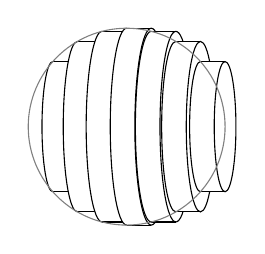
\begin{tikzpicture}
\pgfmathsetmacro{\R}{1.25}
\pgfmathsetmacro{\Ra}{\R/4}
\pgfmathsetmacro{\dR}{\R/4}
\pgfmathsetmacro{\n}{6}
\foreach \x in {-3,-2,-1}{\pgfmathsetmacro{\r}{sqrt(\R^2-(\x*\dR)^2)};\pgfmathsetmacro{\ra}{\r/\n};\pgfmathsetmacro{\xx}{\x*\dR};\fill[white]([shift={(90:\ra cm and \r cm)}]\xx,0) arc (90:270:\ra cm and \r cm)--++(\dR,0)--++(0,2*\r)--++(-\dR,0);\draw([shift={(90:\ra cm and \r cm)}]\xx,0) arc (90:270:\ra cm and \r cm);\draw(\xx,\r)--++(\dR,0)  (\xx,-\r)--++(\dR,0);}
\pgfmathsetmacro{\r}{\R};\pgfmathsetmacro{\ra}{\r/\n};\pgfmathsetmacro{\xx}{0*\dR};\fill[white]([shift={(90:\ra cm and \r cm)}]\xx,0) arc (90:270:\ra cm and \r cm)--++(\dR,0)--++(0,2*\r)--++(-\dR,0);
\foreach \x in {0,1,2,3}{\pgfmathsetmacro{\r}{sqrt(\R^2-(\x*\dR)^2)};\pgfmathsetmacro{\ra}{\r/\n};\pgfmathsetmacro{\xx}{(\x+1)*\dR};\fill[white](\xx,\r)--++(-\dR,0)--++(0,-2*\r)--++(\dR,0)--cycle;
\draw([shift={(90:\ra cm and \r cm)}]\xx-\dR,0) arc (90:270:\ra cm and \r cm);\draw(\xx,0) circle (\ra cm and \r cm);\draw(\xx,\r)--++(-\dR,0) (\xx,-\r)--++(-\dR,0);}
\draw[gray,thin](0,0)circle (\R);
\end{tikzpicture}
\caption{}
\end{subfigure}
\caption{نصف دائرہ \عددی{y=\sqrt{16-x^2}} کو \عددی{x} محور کے گرد گما کر کرہ حاصل کیا جاتا ہے (مثال \حوالہ{مثال_تکمل_حجم_کرہ})۔}
\label{شکل_مثال_تکمل_حجم_کرہ}
\end{figure}


\ابتدا{مثال}\شناخت{مثال_تکمل_حجم_کرہ}
ایک کرہ کا رداس \عددی{4} ہے (شکل \حوالہ{شکل_مثال_تکمل_حجم_کرہ}-ا)۔ اس کا حجم تلاش کریں۔

حل:\quad
ہم تفاعل \عددی{f(x)=\sqrt{16-x^2}} کو \عددی{x} محور کے گرد گما کر کرہ کی سطح حاصل کر سکتے ہیں۔ہم وقفہ \عددی{-4\le x\le 4} کو آٹھ برابر ذیلی وقفوں میں تقسیم کرتے ہیں۔ یوں ایک ذیلی وقفہ کی لمبائی \عددی{\Delta x=1} ہو گی۔ان ذیلی وقفوں کے بائیں سر نقطے \عددی{c_1} تا \عددی{c_7} پر پائے جاتے ہیں (شکل \حوالہ{شکل_مثال_تکمل_حجم_کرہ}-ا)۔ ہم ہر ذیلی وقفہ  کے بائیں سر پر کرہ کے رقبہ عمودی تراش کے برابر رقبہ کا بیلن جس کی لمبائی \عددی{1} ہو لیتے ہیں (شکل \حوالہ{مثال_تکمل_حجم_کرہ}-ب)۔ان تمام بیلنوں  کے حجم کا مجموعہ تقریباً کرہ کے حجم کے برابر ہو گا۔ ہر ایک بیلن کا حجم \عددی{H=\pi r^2h} ہو گا جہاں بیلن کا رداس \عددی{r} اور اس کی لمبائی \عددی{h} ہے۔آٹھوں بیلنوں کے حجم کا مجموعہ درج ذیل ہو گا۔
\begin{align*}
H_8&=\pi[f(x_1)]^2\Delta x+\pi[f(x_2)]^2\Delta x+\pi[f(x_3)]^2\Delta x+\cdots+\pi[f(x_8)]^2\Delta x\\
&=\pi\left[\sqrt{16-x_1^2}\right]^2\Delta x+\pi\left[\sqrt{16-x_2^2}\right]^2\Delta x+\pi\left[\sqrt{16-x_3^2}\right]^2\Delta x+\\
&\quad\quad\cdots+\pi\left[\sqrt{16-x_8^2}\right]^2\Delta x\\
&=\pi[(16-(-4)^2)+(16-(-3)^2)+(16-(-2)^2)+\cdots+(16-(3)^2)]\\
&=\pi[0+7+12+15+16+15+12+7]\\
&=84\pi
\end{align*}
کرہ کا اصل حجم درج ذیل ہے (سوال \حوالہ{سوال_تکمل_حجم_ٹھوس_جسم_ب})۔
\begin{align*}
H=\frac{4}{3}\pi r^3=\frac{4}{3}\pi (4)^3=\frac{256\pi}{3}
\end{align*}
متناہی مجموعہ سے حاصل حجم میں فی صد خلل درج ذیل ہے۔
\begin{align*}
\text{\RL{}}&=\frac{\abs{H-H_8}}{H}\times 100=\frac{\tfrac{256\pi}{3}-84\pi}{\tfrac{256\pi}{3}}\times 100\\
&=\frac{256-252}{256}=\frac{1}{64}\approx \SI{1.6}{\percent}
\end{align*}
\انتہا{مثال}
%==========================

\جزوحصہء{غیر منفی تفاعل کی اوسط قیمت}
متناہی تعداد قیمتوں کی اوسط حاصل کرنے کی خاطر ہم تمام قیمتوں کا مجموعہ لے کر قیمتوں کی تعداد سے تقسیم کرتے ہیں۔ اب لامتناہی تعداد کی قیمتوں کے اوسط سے کیا مراد ہو گا؟ مثال کے طور پر وقفہ \عددی{[-1,1]} پر تفاعل \عددی{f(x)=x^2} کی اوسط قیمت سے کیا مراد ہے؟  ایسے "استمراری" اوسط کا مطلب سمجھنے کی خاطر فرض کریں کہ ہم \عددی{x=-1} تا \عددی{x=1} کے بیچ بلا منصوبہ  \عددی{x} کی مختلف قیمتوں پر تفاعل کی نمونی قیمتوں کے مربع کا اوسط حاصل کرتے ہیں۔ نمونی جسامت بڑھانے سے ہم توقع کرتے ہیں کہ یہ اوسط کسی مخصوص قیمت تک پہنچنے کی کوشش کرے گا۔ اس قیمت کو ہم وقفہ \عددی{[-1,1]} پر تفاعل کا \اصطلاح{اوسط}\فرہنگ{اوسط}\حاشیہب{average}\فرہنگ{average} کہتے ہیں۔

\ابتدا{مثال}\شناخت{مثال_تکمل_استمراری_اوسط}
وقفہ \عددی{[-1,1]} پر تفاعل \عددی{f(x)=x^2} کی اوسط قیمت تلاش کریں۔ 

حل:\quad
ہم وقفہ \عددی{[-1,1]} کو \عددی{6} برابر ذیلی وقفوں میں تقسیم کرتے ہیں (شکل \حوالہ{شکل_مثال_تکمل_استمراری_اوسط})۔ یوں ایک ذیلی وقفہ کی لمبائی \عددی{\Delta x=\tfrac{1}{3}} ہو گی۔

اب تک کی مثالوں میں متناہی مجموعہ حاصل کرتے ہوئے ہم ہر ذیلی وقفہ کے سر پر تفاعل کی قیمت لیتے رہے ہیں۔ اس سے بہتر نتائج اس صورت حاصل ہوتے ہیں جب تفاعل کی قیمت ہر ذیلی وقفہ کی وسط میں لیا جائے۔چھ ذیلی وقفوں کی وسط میں تفاعل کی قیمتوں کے اوسط کی اندازاً قیمت تلاش کرتے ہیں۔
\begin{align*}
\text{\RL{اوسط قیمت}}&\approx \frac{(-\tfrac{5}{6})^2+(-\tfrac{3}{6})^2+(-\tfrac{1}{6})^2+(\tfrac{1}{6})^2+(\tfrac{3}{6})^2+(\tfrac{5}{6})^2}{6}\\
&\approx \frac{1}{6}\cdot \frac{25+9+1+1+9+25}{36}=\frac{70}{216}\approx 0.324
\end{align*} 
اس تفاعل کا اصل اوسط \عددی{\tfrac{1}{3}} ہے۔

درج ذیل پر غور کریں۔
\begin{align*}
 &\frac{(-\tfrac{5}{6})^2+(-\tfrac{3}{6})^2+(-\tfrac{1}{6})^2+(\tfrac{1}{6})^2+(\tfrac{3}{6})^2+(\tfrac{5}{6})^2}{6}\\
&=\frac{1}{2}\left[\big(-\frac{5}{6}\big)^2\cdot\frac{1}{3}+\big(-\frac{3}{6}\big)^2\cdot\frac{1}{3}+\cdots+\big(\frac{5}{6}\big)^2\cdot\frac{1}{3}\right]\\
&=\frac{1}{[-1,1]\, \text{لمبائی}}\cdot \left[f\big(-\frac{5}{6}\big)\cdot\frac{1}{3}+f\big(-\frac{3}{6}\big)\cdot\frac{1}{3}+\cdots+f\big(\frac{5}{6}\big)\cdot\frac{1}{3}\right]\\
&=\frac{1}{[-1,1]\,\text{لمبائی}}\cdot [\text{\RL{تفاعل کی قیمتیں ضرب ذیلی وقفہ کی لمبائی کا مجموعہ}}]
\end{align*}
اس بار بھی اندازاً قیمت حاصل کرنے کی خاطر تفاعل کی قیمت کو ذیلی وقفہ کی لمبائی سے ضرب دیتے ہوئے مجموعہ حاصل کیا گیا ہے۔
\انتہا{مثال}
%========================
\begin{figure}
\centering
\begin{tikzpicture}
\begin{axis}[clip=false,small,axis lines=middle,xlabel={$x$},ylabel={$y$},xmin=-1.25,xmax=1.25,ymax=1.1,xlabel style={at={(current axis.right of origin)},anchor=west},ylabel style={at={(current axis.above origin)},anchor=south},xtick={-1,-0.667,-0.333,0.333,0.667,1},xticklabels={$-1$,$-\tfrac{2}{3}$,$-\tfrac{1}{3}$,$\tfrac{1}{3}$,$\tfrac{2}{3}$,$1$},ytick={1}]
\addplot[domain=-1:1]{x^2}node[left]{$y=x^2$};
\draw(axis cs:-1,0)--(axis cs:-1,1);
\draw(axis cs:-0.667,0)--(axis cs:-0.667,0.4444);
\draw(axis cs:-0.333,0)--(axis cs:-0.333,0.111);
\draw(axis cs:1,0)--(axis cs:1,1);
\draw(axis cs:0.667,0)--(axis cs:0.667,0.4444);
\draw(axis cs:0.333,0)--(axis cs:0.333,0.111);
\draw[dashed](axis cs:-0.1667,0)--(axis cs:-0.1667,0.0278)node[circ]{};
\draw[dashed](axis cs:-0.5,0)--(axis cs:-0.5,0.25)node[circ]{};
\draw[dashed](axis cs:-0.833,0)--(axis cs:-0.833,0.694)node[circ]{};
\draw[dashed](axis cs:0.1667,0)--(axis cs:0.1667,0.0278)node[circ]{};
\draw[dashed](axis cs:0.5,0)--(axis cs:0.5,0.25)node[circ]{};
\draw[dashed](axis cs:0.833,0)--(axis cs:0.833,0.694)node[circ]{};
\end{axis}
\end{tikzpicture}
\caption{تفاعل کا اوسط (مثال \حوالہ{مثال_تکمل_استمراری_اوسط})۔}
\label{شکل_مثال_تکمل_استمراری_اوسط}
\end{figure}

\جزوحصہء{نتیجہ}
اس حصہ میں ہم نے تفاعل کی قیمت کو ذیلی وقفوں کی لمبائی سے ضرب دے کر مجموعہ حاصل کرنے سے درکار قیمتوں کا اندازہ لگایا گیا۔

ہم نے مثال \حوالہ{مثال_تکمل_گولا_طے_فاصلہ_مجموعہ} میں دیکھا کہ ذیلی وقفوں کی لمبائی کم کرنے سے اصل جواب، جس کو ہم الٹ تفرق سے حاصل کر چکے تھے،  کے زیادہ قریب نتائج حاصل ہوتے ہیں۔ کیا ذیلی وقفوں کی لمبائی کم سے کم کرنے سے حاصل نتیجہ کی تحدیدی قیمت اصل جواب تک پہنچتی؟ کیا اس مثال میں مجموعہ اور الٹ تفرق کا تعلق اتفاقی ہے؟ کیا ہم مثال \حوالہ{مثال_تکمل_اخراج_قلب_رقت_رنگ_ترکیب} میں رقبہ، مثال \حوالہ{مثال_تکمل_حجم_عجیب} اور مثال \حوالہ{مثال_تکمل_حجم_کرہ} میں حجم اور مثال \حوالہ{مثال_تکمل_استمراری_اوسط} میں اوسط قیمت کو الٹ تفرق سے حاصل کر سکتے ہیں؟ جیسا ہم دیکھیں گے،  ان سوالات کے جوابات ہیں "جی ہاں ایسا کیا جا سکتا ہے"، "نہیں یہ اتفاق نہیں ہے" اور "جی ہاں ہم ایسا کر سکتے ہیں۔"

\حصہء{سوالات}
\موٹا{اخراج قلب}\\
\ابتدا{سوال}\شناخت{سوال_تکمل_اخراج_قلب_الف}
ایک مریض کے اخراج قلب کو رنگ کی ترکیب سے ناپا گیا۔پیمائش کے نتائج  شکل \حوالہ{شکل_سوال_تکمل_اخراج_قلب_الف}  میں دیے گئے ہیں جہاں خون کی دوبارہ گردش کے اثرات کو مد نظر رکھا گیا ہے۔ ٹیکہ میں رنگ کی مقدار \عددی{\SI{5}{\milli\gram}} تھی۔ کثافت رنگ کی منحنی کے نیچے رقبہ کو مستطیلوں کے رقبوں کا مجموعہ لے کر حاصل کریں۔ اخراج قلب کتنا ہے؟ ( مثال \حوالہ{مثال_تکمل_اخراج_قلب_رقت_رنگ_ترکیب} دیکھیں۔)
\انتہا{سوال}
%=================
\begin{figure}
\centering
\begin{subfigure}{0.45\textwidth}
\centering
\begin{tabular}{C|C}
\toprule
t\,\text{\RL{لمحہ}}&c\,\text{\RL{کثافت رنگ}}\\
\midrule
2&0\\
4&0.6\\
6&1.4\\
8&2.7\\
10&3.7\\
12&4.1\\
14&3.8\\
16&2.9\\
18&1.7\\
20&1.0\\
22&0.5\\
24&0\\
\bottomrule
\end{tabular}
\end{subfigure}\hfill
\begin{subfigure}{0.45\textwidth}
\centering
\begin{tikzpicture}
\begin{axis}[small,axis lines=middle,xlabel={$t(\si{\second})$},ylabel={$c(\si{\milli\gram\per\litre})$}, ymax=4.75,xmax=26,grid=both,xtick={2,4,6,8,10,12,14,16,18,20,22,24}, ytick={0.5,1,1.5,2,2.5,3,3.5,4,4.5}, yticklabels={,$1$,,$2$,,$3$,,$4$},ylabel style={at={(current axis.above origin)},anchor=south}]
\addplot[smooth]plot coordinates {(2,0) (4,0.6) (6,1.4) (8,2.7) (10,3.7) (12,4.1) (14,3.8) (16,2.9) (18,1.7) (20,1.0) (22,0.5) (24,0)};
\draw(axis cs:18,3)node[right]{$c=f(t)$};
\end{axis}
\end{tikzpicture}
\end{subfigure}%
\caption{اخراج قلب جاننے کے لئے کثافت رنگ بالمقابل وقت کی پیمائش (سوال \حوالہ{سوال_تکمل_اخراج_قلب_الف})۔}
\label{شکل_سوال_تکمل_اخراج_قلب_الف}
\end{figure}

\ابتدا{سوال}\شناخت{سوال_تکمل_اخراج_قلب_ب}
ایک مریض کا اخراج قلب جاننے کی خاطر ترکیب رنگ استعمال کیا جاتا ہے۔ کی گئی پیمائش کو جدول \حوالہ{جدول_سوال_تکمل_اخراج_قلب_ب} میں پیش کیا گیا ہے جہاں خوب کی دوبارہ گردش کے اثرات کو مد نظر رکھا گیا ہے۔ ٹیکہ میں رنگ کی مقدار \عددی{\SI{10}{\milli\gram}} ہے۔ پیمائش کو ہموار منحنی سے ترسیم کریں۔ رقبے کا اندازہ مستطیلوں کے رقبوں کا مجموعہ لے کر تلاش کریں۔ اخراج قلب دریافت کریں۔ 
\begin{table}
\caption{وقت بالمقابل کثافت رنگ برائے سوال \حوالہ{سوال_تکمل_اخراج_قلب_ب}۔}
\label{جدول_سوال_تکمل_اخراج_قلب_ب}
\centering
\begin{tabular}{CC|CC}
\toprule
\text{\RL{لمحہ}}&\text{\RL{کثافت رنگ}}&\text{\RL{لمحہ}}&\text{\RL{کثافت رنگ}}\\
t&c&t&c\\
\midrule
0&0&16&7.9\\
2&0&18&7.8\\
4&0.1&20&6.1\\
6&0.6&22&4.7\\
8&2.0&24&3.5\\
10&4.2&26&2.1\\
12&6.3&28&0.7\\
14&7.5&30&0\\
\bottomrule
\end{tabular}
\end{table}
\انتہا{سوال}
%===============
\موٹا{فاصلہ}\\
\ابتدا{سوال}\شناخت{سوال_تکمل_رفتار_ریل_گاڑی}
ایک ریل گاڑی کی رفتار بالمقابل وقت شکل \حوالہ{شکل_سوال_تکمل_رفتار_ریل_گاڑی}-ا میں دی گئی ہے۔ دس سیکنڈ وقفے کو \عددی{10} برابر ذیلی وقفوں میں تقسیم کرتے ہوئے ہر ذیلی وقفہ  کے (ا) بائیں سر، (ب) دائیں سر پر قیمتیں لیتے ہوئے طے فاصل تلاش کریں۔\\
جواب:\quad
(ا) \عددی{\SI{87}{\meter}}، (ب) \عددی{86\meter}
\انتہا{سوال}
%====================
\begin{figure}
\centering
\begin{subfigure}{0.45\textwidth}
\centering
\begin{tabular}{@{}CC|CC@{}}
\toprule
\text{لمحہ}&\text{رفتار}&\text{لمحہ}&\text{رفتار}\\
t(\si{\second})&v(\si{\meter\per\second})&t(\si{\second})&v(\si{\meter\per\second})\\
\midrule
0&0&6&11\\
1&12&7&6\\
2&22&8&2\\
3&10&9&6\\
4&5&10&0\\
5&13&&\\
\bottomrule
\end{tabular}
\caption{رفتار بالمقابل وقت برائے سوال \حوالہ{سوال_تکمل_رفتار_ریل_گاڑی}}
\end{subfigure}\hfill
\begin{subfigure}{0.45\textwidth}
\centering
\begin{tabular}{@{}CC|CC@{}}
\toprule
\text{لمحہ}&\text{رفتار}&\text{لمحہ}&\text{رفتار}\\
t(\si{\minute})&v(\si{\meter\per\second})&t(\si{\minute})&v(\si{\meter\per\second})\\
\midrule
0&1&35&1.2\\
5&1.2&40&1.0\\
10&1.7&45&1.8\\
15&2.0&50&1.5\\
20&1.8&55&1.2\\
25&1.6&60&0\\
30&1.4&&\\
\bottomrule
\end{tabular}
\caption{رفتار بالمقابل وقت برائے سوال \حوالہ{سوال_تکمل_رفتار_بوتل}}
\end{subfigure}
\caption{رفتار بالمقابل وقت کی پیمائشی قیمتیں۔}
\label{شکل_سوال_تکمل_رفتار_ریل_گاڑی}
\end{figure}

\ابتدا{سوال}\شناخت{سوال_تکمل_رفتار_بوتل}
نہر کے پانی میں ایک بوتل کی رفتار بالمقابل وقت کو شکل \حوالہ{شکل_سوال_تکمل_رفتار_ریل_گاڑی}-ب میں دیا گیا ہے۔ ایک گھنٹہ کے وقفہ کو \عددی{12} برابر ذیلی وقفوں میں تقسیم کریں۔ ان ذیلی وقفوں کے (ا) بائیں سر قیمتیں، (ب) دائیں سر قیمتیں استعمال کرتے ہوئے وہ  فاصل تلاش کریں جو بوتل اس گھنٹہ میں طے کرتا ہے۔ 
\انتہا{سوال}
%==========================
\ابتدا{سوال}\شناخت{سوال_تکمل_گاڑی_رفتار_الف}
ایک گاڑی جس کا رفتار پیما کار آمد لیکن مسافت پیما غیر کارآمد ہے میں آپ سفر کر رہے ہیں۔ آپ ہر \عددی{10} سیکنڈ اس کی رفتار قلم بند کرتے ہیں۔ ان نتائج کو شکل \حوالہ{شکل_سوال_تکمل_گاڑی_رفتار_الف}-ا میں دکھایا گیا ہے۔ سڑک کی لمبائی کی اندازاً قیمت کو (ا) بائیں سر نقطی قیمتیں، (ب) دائیں سر نقطی قیمتیں استعمال کرتے ہوئے تلاش کریں۔\\
جواب:\quad
(ا) \عددی{\SI{969}{\meter}}، (ب) \عددی{\SI{1067}{\meter}}
\انتہا{سوال}
%========================
\begin{figure}
\centering
\begin{subfigure}{0.45\textwidth}
\centering
\begin{tabular}{CC|CC}
\toprule
\text{لمحہ}&\text{رفتار}&\text{لمحہ}&\text{رفتار}\\
\text{سیکنڈ}& \si{\kilo\meter\per\hour}&\text{سیکنڈ}& \si{\kilo\meter\per\hour}\\
\midrule
0&0&70&15\\
10&44&80&22\\
20&15&90&35\\
30&35&100&44\\
40&30&110&30\\
50&44&120&35\\
60&35&&\\
\bottomrule
\end{tabular}
\caption{برائے سوال \حوالہ{سوال_تکمل_گاڑی_رفتار_الف}}
\end{subfigure}\hfill
\begin{subfigure}{0.45\textwidth}
\centering
\begin{tabular}{CC|CC}
\toprule
\text{لمحہ}&\text{رفتار}&\text{لمحہ}&\text{رفتار}\\
\text{گھنٹے}& \si{\kilo\meter\per\hour}&\text{گھنٹے}& \si{\kilo\meter\per\hour}\\
\midrule
0&0&0.006&116\\
0.001&40&0.007&125\\
0.002&62&0.008&132\\
0.003&82&0.009&137\\
0.004&96&0.010&142\\
0.005&108&&\\
\bottomrule
\end{tabular}
\caption{برائے سوال \حوالہ{سوال_تکمل_گاڑی_رفتار_ب}}
\end{subfigure}%
\caption{گاڑی کی رفتار بالمقابل وقت۔}
\label{شکل_سوال_تکمل_گاڑی_رفتار_الف}
\end{figure}
\ابتدا{سوال}\شناخت{سوال_تکمل_گاڑی_رفتار_ب}
ساکن حال سے \عددی{36} سیکنڈ میں ایک گاڑی \عددی{\SI{142}{\kilo\meter\per\hour}} کی رفتار تک پہنچتی ہے۔ اس کی رفتار بالمقابل وقت کو شکل \حوالہ{شکل_سوال_تکمل_گاڑی_رفتار_الف}-ب میں دکھایا گیا ہے۔ (ا) مستطیل استعمال کرتے ہوئے ان \عددی{36} سیکنڈوں میں طے شدہ فاصلہ تلاش کریں۔ (ب)  گاڑی تقریباً کتنی دیر میں آدھے فاصلہ تک پہنچی؟  اس لمحے پر گاڑی کی رفتار کتنی تھی؟
\انتہا{سوال}
%========================
\ابتدا{سوال}\شناخت{سوال_تکمل_حجم_دو_ٹکڑے}
فرض کریں ہم مثال \حوالہ{مثال_تکمل_حجم_عجیب} میں حجم کا اندازہ صرف \عددی{2} چکور بیلنوں سے کرتے ہیں (شکل \حوالہ{شکل_سوال_تکمل_حجم_دو_ٹکڑے}-ا)۔ (ا) حجم \عددی{H_2} تلاش کریں۔ (ب) خلل \عددی{\abs{H-H_2}}  کی \عددی{H} کے لحاظ سے فی صد قیمت حاصل کریں۔   
\انتہا{سوال}
%=======================
\begin{figure}
\centering
\begin{subfigure}{0.45\textwidth}
\centering
\begin{tikzpicture}
\pgfmathsetmacro{\w}{4}
\pgfmathsetmacro{\h}{1.5}
\draw[-latex](-0.5,0)--(4.5,0)node[right]{$x$};
\draw[thick](0,0)node[circ]{}node[below]{$-2$}--++(0,\h) to [out=55,in=125]coordinate[pos=0.5](kT)++(\w,0)--++(0,-\h)node[below]{$2$};
\draw(0,\h)--++(\w/2,0);
\draw(kT)--($(0,0)!(kT)!(\w,0)$)node[circ]{}node[below]{$0$};
\draw(kT)--++(\w/2,0)coordinate(kTT)--($(0,0)!(kTT)!(\w/2+0.2,0)$);
\end{tikzpicture}
\caption{جسم کے حجم کو \عددی{2} چکور بیلنوں کے حجم کے مجموعہ سے حاصل کیا گیا ہے۔}
\end{subfigure}\hfill
\begin{subfigure}{0.45\textwidth}
\centering
\begin{tikzpicture}
\pgfmathsetmacro{\w}{4}
\pgfmathsetmacro{\h}{1.5}
\pgfmathsetmacro{\ww}{\w/6}
\draw[-latex](-0.5,0)--(4.5,0)node[right]{$x$};
\draw[thick,name path=dome](0,0)node[circ]{}node[below]{$-2$}--++(0,\h) to [out=55,in=125]++(\w,0)--++(0,-\h)node[below]{$2$};
\path[name path=kA](1*\ww,0)--++(0,1.75*\h);
\path[name path=kB](2*\ww,0)--++(0,1.75*\h);
\path[name path=kC](3*\ww,0)--++(0,1.75*\h);
\path[name path=kD](4*\ww,0)--++(0,1.75*\h);
\path[name path=kE](5*\ww,0)--++(0,1.75*\h);
\draw[name intersections={of=dome and kA}] (1*\ww,0)node[circ]{}node[below]{$-\tfrac{4}{3}$}--(intersection-1)coordinate(kAA);
\draw[name intersections={of=dome and kB}] (2*\ww,0)node[circ]{}node[below]{$-\tfrac{2}{3}$}--(intersection-1)coordinate(kBB);
\draw[name intersections={of=dome and kC}] (3*\ww,0)node[circ]{}node[below]{$0$}--(intersection-1)coordinate(kCC);
\draw[name intersections={of=dome and kD}] (4*\ww,0)node[circ]{}node[below]{$\tfrac{2}{3}$}--(intersection-1)coordinate(kDD);
\draw[name intersections={of=dome and kE}] (5*\ww,0)node[circ]{}node[below]{$\tfrac{4}{3}$}--(intersection-1)coordinate(kEE);
\draw(0,\h)--++(\ww,0);
\draw(kAA)--++(\ww,0);
\draw(kBB)--++(\ww,0);
\path[name path=topC](kCC)--++(3*\ww+0.2,0);
\path[name path=topD](kDD)--++(2*\ww+0.2,0);
\path[name path=topE](kEE)--++(1*\ww+0.2,0);
%
\path[name path=RD](kDD)--++(0,0.2);
\path[name path=RE](kEE)--++(0,0.4);
\path[name path=RF](\w,\h)--++(0,0.8);
%
\draw[name intersections={of=topC and RD}](kDD)--(intersection-1)--++(-\ww,0);
\draw[name intersections={of=topD and RE}](kEE)--(intersection-1)--++(-\ww,0)--(kDD);
\draw[name intersections={of=topE and RF}](\w,\h)--(intersection-1)--++(-\ww,0)--(kEE);
\end{tikzpicture}
\caption{جسم کے حجم کو \عددی{6} چکور بیلنوں کے حجم کے مجموعہ سے حاصل کیا گیا ہے۔}
\end{subfigure}
\caption{حجم کے ذیلی وقفے (سوال \حوالہ{سوال_تکمل_حجم_دو_ٹکڑے} اور سوال \حوالہ{سوال_تکمل_حجم_چھ_ٹکڑے})}
\label{شکل_سوال_تکمل_حجم_دو_ٹکڑے}
\end{figure}
\ابتدا{سوال}\شناخت{سوال_تکمل_حجم_چھ_ٹکڑے}
فرض کریں ہم مثال \حوالہ{مثال_تکمل_حجم_عجیب} میں حجم کا اندازہ صرف \عددی{6} چکور بیلنوں سے کرتے ہیں (شکل \حوالہ{شکل_سوال_تکمل_حجم_دو_ٹکڑے}-ب)۔ (ا) حجم \عددی{H_6} تلاش کریں۔ (ب) خلل \عددی{\abs{H-H_6}} کو \عددی{H} کی فی صد کی صورت میں حاصل کریں۔  
\انتہا{سوال}
%=====================
\ابتدا{سوال}
فرض کریں ہم مثال \حوالہ{مثال_تکمل_حجم_کرہ} میں کرہ کا حجم حاصل کرنے کے لئے وقفہ \عددی{-4\le x\le 4} کو چار برابر ذیلی وقفوں میں تقسیم کرتے ہیں۔ہم ہر ذیلی وقفہ  کے بائیں سر نقطہ پر رقبہ عمودی تراش کے برابر بیلن لیتے ہیں۔ (بائیں ترین بیلن کا رقبہ عمودی تراش صفر ہو گا۔) (ا) ان بیلنوں کا مجموعی حجم \عددی{H_4} تلاش کریں۔ (ب) خلل \عددی{\abs{H-H_4}} کو \عددی{H} کا فی صد لکھیں؟
\انتہا{سوال}
%=====================
\ابتدا{سوال}
ایک کرہ جس کا رداس \عددی{5} ہے کا حجم درکار ہے۔ آپ اس کے قطر کو پانچ برابر ذیلی وقفوں میں تقسیم کرتے ہیں۔یوں ایک ذیلی وقفہ \عددی{2} کے برابر ہو گا۔ آپ ان ذیلی وقفوں  کے بائیں سر نقطوں پر قطر کے عمودی  کرہ کو کاٹ کر رقبہ عمودی تراش حاصل کرتے ہیں۔ آپ اتنی ہی رقبہ عمودی تراش والے ایسے بیلن لیتے ہیں جن کی موٹائی \عددی{2} ہو۔ان بیلنوں کے مجموعی حجم سے آپ کرہ کے حجم کی اندازاً قیمت تلاش کرتے ہیں۔ (ا) بیلنوں کا مجموعی حجم \عددی{H_5} کیا ہو گا؟ (ب)  خلل \عددی{\abs{H-H_5}} کو \عددی{H} کا فی صد لکھیں۔
\انتہا{سوال}
%=====================
\ابتدا{سوال}\شناخت{سوال_تکمل_کرہ_نصف}
رداس \عددی{4} کے کرہ کا حجم درکار ہے۔ اس کا محور تشاکل \عددی{x} محور پر  وقفہ \عددی{[0,4]} ہے۔ آپ اس وقفہ کو \عددی{8} برابر ذیلی وقفوں میں تقسیم کرتے ہیں۔ ہر ذیلی وقفہ  کے بائیں سر نقطہ پر کرہ کے رقبہ عمودی تراش کے برابر بیلن جس کی موٹائی ذیلی وقفہ کی لمبائی جتنی ہو کو استعمال کرتے ہوئے کرہ کا حجم تلاش کیا جاتا ہے (شکل \حوالہ{شکل_سوال_تکمل_کرہ_نصف})۔ (ا) مجموعی حجم \عددی{H_8} تلاش کریں (جو نصف کرہ کا حجم ہو گا)۔ (ب) کیا \عددی{H_8} نصف کرہ کے حجم \عددی{H} سے کم یا زیادہ ہو گا؟ اپنے جواب کی وجہ پیش کریں۔ (ب) خلل \عددی{\abs{H-H_8}} کو \عددی{H} کا فی صد لکھیں۔
\انتہا{سوال}
%=================
\begin{figure}
\centering
\begin{minipage}{0.45\textwidth}
\begin{tikzpicture}
\pgfmathsetmacro{\r}{1.25}
\pgfmathsetmacro{\xx}{\r/8}
\pgfmathsetmacro{\yA}{sqrt(\r^2-(1*\xx)^2)}
\pgfmathsetmacro{\yB}{sqrt(\r^2-(2*\xx)^2)}
\pgfmathsetmacro{\yC}{sqrt(\r^2-(3*\xx)^2)}
\pgfmathsetmacro{\yD}{sqrt(\r^2-(4*\xx)^2)}
\pgfmathsetmacro{\yE}{sqrt(\r^2-(5*\xx)^2)}
\pgfmathsetmacro{\yF}{sqrt(\r^2-(6*\xx)^2)}
\pgfmathsetmacro{\yG}{sqrt(\r^2-(7*\xx)^2)}
\draw[-latex](-0.25,0)--(1.5*\r,0)node[right]{$x$};
\draw[-latex](0,-1.1*\r)--(0,1.15*\r)node[above]{$y$};
\draw([shift={(-90:\r)}]0,0) arc (-90:90:\r);
\draw(0,\r)--++(\xx,0)--++(0,-2*\r)--++(-\xx,0);
\draw(1*\xx,\yA)--++(\xx,0)--++(0,-2*\yA)--++(-\xx,0);
\draw(2*\xx,\yB)--++(\xx,0)--++(0,-2*\yB)--++(-\xx,0);
\draw(3*\xx,\yC)--++(\xx,0)--++(0,-2*\yC)--++(-\xx,0);
\draw(4*\xx,\yD)--++(\xx,0)--++(0,-2*\yD)--++(-\xx,0);
\draw(5*\xx,\yE)--++(\xx,0)--++(0,-2*\yE)--++(-\xx,0);
\draw(6*\xx,\yF)--++(\xx,0)--++(0,-2*\yF)--++(-\xx,0);
\draw(7*\xx,\yG)--++(\xx,0)--++(0,-2*\yG)--++(-\xx,0);
\foreach \x in {0,1,2,3,4,5,6,7}{\draw(\x*\xx,0)node[circ]{};}
\draw(0,0)node[below left]{$0$};
\draw(\r,0)node[below right]{$4$};
\draw(\r,2/3*\r)node[right,font=\small]{$y=\sqrt{16-x^2}$};
\end{tikzpicture}
\caption{نصف کرہ (سوال \حوالہ{سوال_تکمل_کرہ_نصف})}
\label{شکل_سوال_تکمل_کرہ_نصف}
\end{minipage}\hfill
\begin{minipage}{0.45\textwidth}
\centering
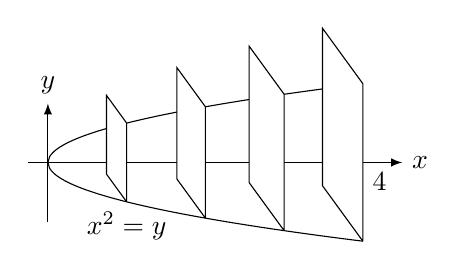
\begin{tikzpicture}[declare function={f(\x)=sqrt(\x);},y=0.5cm]
\pgfmathsetmacro{\ang}{110}
\draw[-latex](-0.25,0)--(4.5,0)node[right]{$x$};
\draw[-latex](0,-1.5)--(0,1.5)node[above]{$y$};
\draw[domain=0:0.5]plot (\x,{f(\x)});
\draw[domain=0:0.5]plot(\x,{-f(\x)});
\draw[domain=0.5:4]plot (\x,{f(\x)});
\draw[domain=0.5:4]plot(\x,{-f(\x)});
\foreach \x in {1,2,3,4}{\pgfmathsetmacro{\y}{f(\x)};\draw[fill=white](\x,-\y)--(\x,\y)--++(\ang:0.75*\y)--++(0,-2*\y)--++(\ang:-0.75*\y);}
\draw(4,0)node[below right]{$4$};
\draw(1,-1)node[below]{$x^2=y$};
\end{tikzpicture}
\caption{برائے سوال \حوالہ{سوال_تکمل_بہت_زیادہ_خلل_چکور}}
\label{شکل_سوال_تکمل_بہت_زیادہ_خلل_چکور}
\end{minipage}
\end{figure}
\ابتدا{سوال}
گزشتہ سوال (سوال \حوالہ{سوال_تکمل_کرہ_نصف}) میں ہر ذیلی وقفہ کے دائیں سر نقطے پر رقبہ عمودی تراش کے برابر بیلن لیتے ہوئے  دوبارہ جوابات حاصل کریں۔
\انتہا{سوال}
%=======================
\ابتدا{سوال}\شناخت{سوال_تکمل_بہت_زیادہ_خلل_چکور}\ترچھا{اندازاً حجم میں بہت زیادہ خلل}\\
نقطہ \عددی{x=0} اور \عددی{x=4} پر \عددی{x} محور کے عمودی سطحوں کے بیچ ایک ٹھوس جسم پایا جاتا ہے۔ اس محور کے عمودی جسم کا رقبہ عمودی تراش چکور ہے جس کے کنارے  قطع مکافی \عددی{y=-\sqrt{x}} اور \عددی{y=\sqrt{x}} کو مس کرتے ہیں (شکل \حوالہ{شکل_سوال_تکمل_بہت_زیادہ_خلل_چکور})۔ (ا) وقفہ \عددی{0\le x\le 4} کو چار برابر ذیلی وقفوں میں تقسیم کرتے ہوئے دائیں سر نقطی رقبہ عمودی تراش لیتے ہوئے حجم \عددی{H_4} تلاش کریں۔ اصل حجم \عددی{H=32} ہے۔ خلل \عددی{\abs{H-H_4}} کو \عددی{H} کے لحاظ سے فی صد کی صورت میں لکھیں۔ (ج) اس مسئلے کو دوبارہ \عددی{H_8} کے لئے حل کریں۔
\انتہا{سوال}
%=========================
\begin{figure}
\centering
\begin{minipage}{0.45\textwidth}
\centering
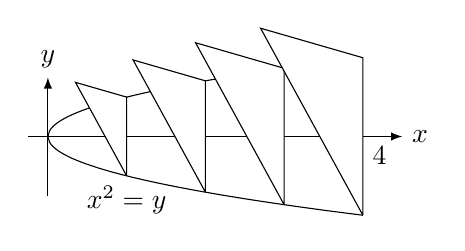
\begin{tikzpicture}[declare function={f(\x)=sqrt(\x);},y=0.5cm]
\pgfmathsetmacro{\ang}{150}
\draw[-latex](-0.25,0)--(4.5,0)node[right]{$x$};
\draw[-latex](0,-1.5)--(0,1.5)node[above]{$y$};
\draw[domain=0:0.5]plot (\x,{f(\x)});
\draw[domain=0:0.5]plot(\x,{-f(\x)});
\draw[domain=0.5:4]plot (\x,{f(\x)});
\draw[domain=0.5:4]plot(\x,{-f(\x)});
\foreach \x in {1,2,3,4}{\pgfmathsetmacro{\y}{f(\x)};\draw[fill=white](\x,-\y)--(\x,\y)--++(\ang:0.75*\y)--(\x,-\y);}
\draw(4,0)node[below right]{$4$};
\draw(1,-1)node[below]{$x^2=y$};
\end{tikzpicture}
\caption{برائے سوال \حوالہ{سوال_تکمل_بہت_زیادہ_خلل_تکون}}
\label{شکل_سوال_تکمل_بہت_زیادہ_خلل_تکون}
\end{minipage}\hfill
\begin{minipage}{0.45\textwidth}
\centering
\begin{tikzpicture}[declare function={f(\x)=sqrt(\x);},scale=0.75]
\pgfmathsetmacro{\n}{6}
\draw[-latex](-0.25,0)--(6,0)node[right]{$x$};
\draw[-latex](0,-2)--(0,2)node[above]{$y$};
\draw[domain=0:0.5] plot ({\x},{f(\x)});
\draw[domain=0:0.5] plot ({\x},{-f(\x)});
\draw[domain=0.5:5] plot ({\x},{f(\x)});
\draw[domain=0.5:5] plot ({\x},{-f(\x)});
\foreach \x in {1,2,3,4}{\pgfmathsetmacro{\y}{f(\x)};\pgfmathsetmacro{\ya}{\y/\n};\fill[fill=white]([shift={(90:\ya cm and \y cm)}]\x,0) arc (90:270:\ya cm and \y cm)--++(1,0)--++(0,2*\y)--++(-1,0);\draw[]([shift={(90:\ya cm and \y cm)}]\x,0) arc (90:270:\ya cm and \y cm)--++(1,0)++(0,2*\y)--++(-1,0);\draw(\x+1,0) circle (\ya cm and \y cm);}
\draw(1,-2)node[]{$x^2=y$};
\draw(5,0)node[below]{$5$};
\draw[gray](4-0.2,0)--++(0.4,0);
\draw[stealth-stealth,gray](4,0)node[circ]{}node[below]{$4$}--++(0,2)node[pos=0.5,fill=white]{$4$};
\end{tikzpicture}
\caption{راکٹ کی نوک (سوال \حوالہ{سوال_تکمل_راکٹ_نوک})}
\label{شکل_سوال_تکمل_راکٹ_نوک}
\end{minipage}
\end{figure}

\ابتدا{سوال}\شناخت{سوال_تکمل_بہت_زیادہ_خلل_تکون}\ترچھا{اندازاً حجم میں بہت زیادہ خلل}\\
نقطہ \عددی{x=0} اور \عددی{x=4} پر \عددی{x} محور کے عمودی سطحوں کے بیچ ایک ٹھوس جسم پایا جاتا ہے۔ اس محور کے عمودی جسم کا رقبہ عمودی تراش متساوی الاضلاع شکل کا ہے جس کے قاعدہ  قطع مکافی \عددی{y=-\sqrt{x}} اور \عددی{y=\sqrt{x}} کو مس کرتا ہے (شکل \حوالہ{شکل_سوال_تکمل_بہت_زیادہ_خلل_تکون})۔(ا) وقفہ \عددی{0\le x\le 4} کو چار برابر ذیلی وقفوں میں تقسیم کرتے ہوئے بائیں سر نقطی رقبہ عمودی تراش لیتے ہوئے حجم \عددی{H_4} تلاش کریں۔ اصل حجم \عددی{H=8\sqrt{3}} ہے۔ \عددی{H} کے لحاظ سے خلل \عددی{\abs{H-H_4}} کی فی صد قیمت کتنی ہے؟ (ج) سوال کو دوبارہ \عددی{H_8} کے لئے حل کریں۔
\انتہا{سوال}
%=====================
\ابتدا{سوال}\شناخت{سوال_تکمل_نصف_کروی_ٹینکی_میں_پانی}
ایک پانی کی ٹینکی نصف کروی پیالے کی مانند ہے جس کا رداس \عددی{\SI{8}{\meter}} ہے۔اس میں پانی کی گہرائی \عددی{\SI{4}{\meter}} ہے۔ (ا) پانی کی گہرائی کو آٹھ ذیلی وقفوں میں تقسیم کرتے ہوئے ہر ذیلی وقفے کی نچلی سطح کا رقبہ عمودی تراش والے بیلن استعمال کرتے ہوئے \عددی{H_8} تلاش کریں۔  (ب)  اصل حجم جو آپ سوال \حوالہ{سوال_تکمل_حجم_ٹھوس_جسم_پ} میں تلاش کریں گے  \عددی{H=\tfrac{320\pi}{3}\,\si{\meter\cubed}} ہے۔ \عددی{H} کے لحاظ سے خلل \عددی{\abs{H-H_8}} کی فی صد قیمت تلاش کریں۔
\انتہا{سوال}
%======================
\ابتدا{سوال}\شناخت{سوال_تکمل_تالاب}
تیراکی کے ایک مستطیل تالاب کی لمبائی \عددی{\SI{10}{\meter}} اور چوڑائی \عددی{\SI{6}{\meter}} ہے۔ تالاب کے ایک سر سے دوسرے سر تک \عددی{\SI{1}{\meter}} وقفوں پر پانی کی گہرائی (میٹر) جدول \حوالہ{جدول_سوال_تکمل_تالاب} میں دی گئی ہے۔ (ا) \عددی{h} کی بائیں سر نقطی قیمتیں استعمال کرتے ہوئے تالاب میں پانی کا حجم  تلاش کریں۔ (ب) دائیں سر نقطی قیمت استعمال کرتے ہوئے حجم تلاش کریں۔
\انتہا{سوال}
%========================
\begin{table}
\caption{تالاب میں پانی کی گہرائی (سوال \حوالہ{سوال_تکمل_تالاب})}
\label{جدول_سوال_تکمل_تالاب}
\centering
\begin{tabular}{CC|CC}
\toprule
\text{مقام}&\text{گہرائی}&\text{مقام}&\text{گہرائی}\\
x&h&x&h\\
\midrule
0&2.0&6&3.83\\
1&2.73&7&3.97\\
2&3.03&8&4.1\\
3&3.3&9&4.23\\
4&3.5&10&4.33\\
5&3.67&&\\
\bottomrule
\end{tabular}
\end{table}

%==================

\ابتدا{سوال}\شناخت{سوال_تکمل_راکٹ_نوک}
منحنی \عددی{y=\sqrt{x},\,0\le x\le 5} کو \عددی{y} محور کے گرد گمانے سے ایک راکٹ کی قطع مکافی مجسم نوک حاصل ہوتی ہے جہاں \عددی{x} کی پیمائش میٹروں میں ہے (شکل \حوالہ{شکل_سوال_تکمل_راکٹ_نوک})۔ اس نوک کا حجم معلوم کرنے کی خاطر ہم \عددی{[0,5]} کو پانچ  برابر حصوں میں تقسیم کرتے ہیں۔یوں ہر حصے کی لمبائی \عددی{1} ہو گی۔ ہر حصہ کے بائیں سر نقطہ پر \عددی{x} محور کے قائمہ جسم کو کاٹا جاتا ہے اور ان نقطوں پر جسم کے رقبہ عمودی تراش کے برابر بیلن استعمال کرتے ہوئے نوک کا حجم دریافت کیا جاتا ہے۔ بیلنوں کی لمبائی \عددی{1} ہو گی۔ (ا) مجموعہ \عددی{H_5} تلاش کریں۔ کیا \عددی{H_5} کی قیمت \عددی{H} سے کم یا زیادہ ہو گی؟ اپنے جواب کی وجہ پیش کریں۔ (ب) نوک کا اصل حجم جو آپ سوال \حوالہ{سوال_تکمل_حجم_ٹھوس_جسم_ت} میں تلاش کریں گے  \عددی{H=2\pi\,\si{\meter\cubed}} ہے۔ خلل \عددی{\abs{H-H_5}} کو \عددی{H} کے فی صد کی صورت میں لکھیں۔ \\
جواب:\quad
(ا) \عددی{1.6\pi}، (ب) \عددی{\SI{20}{\percent}}
\انتہا{سوال}
%======================
\ابتدا{سوال}
ہر ذیلی وقفے کے دائیں سر نقطی رقبہ عمودی تراش استعمال کرتے ہوئے سوال \حوالہ{سوال_تکمل_راکٹ_نوک} کو دوبارہ حل کریں۔
\انتہا{سوال}
%======================
\موٹا{تفاعل کی اوسط قیمت}\\
سوال \حوالہ{سوال_تکمل_تفاعل_اوسط_الف} تا سوال \حوالہ{سوال_تکمل_تفاعل_اوسط_ب} میں تفاعل \عددی{f} کی اوسط قیمت درکار ہے۔دیے گئے وقفہ کو چار ذیلی وقفوں میں تقسیم کرتے ہوئے ہر ذیلی وقفے کی وسط میں تفاعل کی قیمت استعمال کرتے ہوئے متناہی مجموعہ استعمال کرتے ہوئے اوسط حاصل کریں۔

\ابتدا{سوال}\شناخت{سوال_تکمل_تفاعل_اوسط_الف}
$f(x)=x^3,\quad [0,1]$
\انتہا{سوال}
%=====================
\ابتدا{سوال}
$f(x)=\tfrac{1}{x},\quad [1,9]$
\انتہا{سوال}
%=====================
\ابتدا{سوال}\شناخت{سوال_تکمل_تفاعل_اوسط_پ}
$f(t)=\tfrac{1}{2}\sin^2\pi t,\quad [0,2]$ 
شکل \حوالہ{شکل_سوال_تکمل_تفاعل_اوسط_پ}
\انتہا{سوال}
%======================
\ابتدا{سوال}\شناخت{سوال_تکمل_تفاعل_اوسط_ب}
$f(t)=1-(\cos\tfrac{\pi t}{4})^4,\quad [0,4]$
شکل \حوالہ{شکل_سوال_تکمل_تفاعل_اوسط_ب}
\انتہا{سوال}
%=================
\begin{figure}
\centering
\begin{minipage}{0.45\textwidth}
\centering
\begin{tikzpicture}
\begin{axis}[clip=false,small,axis lines=middle,xlabel={$t$},ylabel={$y$},ymin=0,xmax=2.5,ymax=1.75]
\addplot[domain=0:2,smooth]{1/2+(sin(deg(pi*x)))^2};
\draw(axis cs:1,0.3)node[font=\small]{$y=\tfrac{1}{2}+\sin^2\pi t$};
\end{axis}
\end{tikzpicture}
\caption{ترسیم برائے سوال \حوالہ{سوال_تکمل_تفاعل_اوسط_پ}}
\label{شکل_سوال_تکمل_تفاعل_اوسط_پ}
\end{minipage}\hfill
\begin{minipage}{0.45\textwidth}
\centering
\begin{tikzpicture}
\begin{axis}[clip=false,small,axis lines=middle,xlabel={$t$},ylabel={$y$},xmax=4.5,ymax=1.25]
\addplot[domain=0:4,smooth]{1-(cos(deg(pi*x/4)))^4};
\draw(axis cs:2,0.3)node[font=\small]{$y=1-\big(\cos\tfrac{\pi t}{4}\big)^4$};
\end{axis}
\end{tikzpicture}
\caption{ترسیم برائے سوال \حوالہ{سوال_تکمل_تفاعل_اوسط_ب}}
\label{شکل_سوال_تکمل_تفاعل_اوسط_ب}
\end{minipage}
\end{figure}

\موٹا{رفتار اور فاصلہ}\\
\ابتدا{سوال}
ایک جسم کو جہاز سے گرنے دیا جاتا ہے۔ جسم کی رفتار مسلسل بڑھتی ہے لیکن ہوائی رگڑ کی بنا گرنے کی اسراع بتدریج کم ہوتی جاتی ہے۔ وقت بالمقابل جسم کی اسراع کو درج ذیل جدول میں پیش کیا گیا ہے۔
\begin{align*}
\begin{array}{c|cccccc}
t(\si{\second})&0&1&2&3&4&5\\
\hline
a(\si{\meter\per\second\squared})&9.8&5.92&3.59&2.18&1.32&0.80
\end{array}
\end{align*} 
(ا) لمحہ \عددی{t=5} پر رفتار کی بالائی حد تلاش کریں۔ (ب) لمحہ \عددی{t=5} پر رفتار کی نچلی حد تلاش کریں۔ (ج) لمحہ \عددی{t=3} میں گرنے والے فاصلہ کی بالائی حد تلاش کریں۔\\ 
جواب:\quad
(ا) \عددی{\SI{22.81}{\meter\per\second}}، (ب) \عددی{\SI{13.81}{\meter\per\second}}، (ج) \عددی{\SI{35.175}{\meter}}
\انتہا{سوال}
%====================
\ابتدا{سوال}
ایک جسم کو سمندری سطح سے سیدھا اوپر \عددی{\SI{125}{\meter\per\second}} کی رفتار سے  پھینکا جاتا ہے۔ فرض کریں کہ اس جسم پر صفر ثقلی قوت اثر انداز ہوتی ہے۔ (ا) پانچ سیکنڈ بعد اس کی رفتار کی بالائی حد تلاش کریں۔ (ب) پانچ سیکنڈ بعد اس کی رفتار کی نچلی حد تلاش کریں۔ ثقلی اسراع کو \عددی{\SI{9.8}{\meter\per\second\squared}} لیں۔
\انتہا{سوال}
%================
\موٹا{آلودگی پر قابو پانا}\\
\ابتدا{سوال}
تیل کے جہاز سے سمندر میں تیل رس رہا ہے۔ رستا تیل کی مقدار (لٹر فی گھنٹہ) بالمقابل وقت (گھنٹہ) کو نیچے جدول میں دیا گیا ہے۔آپ دیکھ سکتے ہیں کہ صورت حال بتدریج خراب ہو رہی ہے۔
\begin{align*}
\begin{array}{c|ccccccccc}
\text{گھنٹہ}&0&1&2&3&4&5&6&7&8\\
\hline
\si{\litre\per\hour}&50&70&97&136&190&265&369&516&720
\end{array}
\end{align*} 
(ا) ان پانچ گھنٹوں میں خارج تیل کی مقدار کی بالائی اور نچلی حد تلاش کریں۔ (ب) آٹھ گھنٹوں میں خارج تیل کی بالائی اور نچلی حد تلاش  کریں۔ (ج) ابتدائی آٹھ گھنٹوں بعد تیل مسلسل \عددی{\SI{720}{\litre\per\hour}} سے رستا ہے۔ اگر جہاز میں ابتدائی طور کل \عددی{\SI{25000}{\litre}} تیل ہو تب تمام تیل خارج ہونے کے لئے زیادہ سے زیادہ اور کم سے کم  کتنا وقت درکار ہو گا۔ \\
جواب:\quad
(ا) \عددی{\SI{758}{\litre}}، \عددی{\SI{543}{\litre}}، (ب) \عددی{\SI{2363}{\litre}}، \عددی{\SI{1693}{\litre}}، (ج) \عددی{\SI{31.4}{\hour}}، \عددی{\SI{32.4}{\hour}}
\انتہا{سوال}
%======================
\ابتدا{سوال}
ایک بجلی گھر تیل کو جلا کر برقی طاقت پیدا کرتا ہے۔ تیل جلنے سے پیدا آلودگی کو کم کرنے کی خاطر دھواں کش کو چھلنی سے گزارا جاتا ہے جو نجاست کو روک دیتا ہے۔ وقت کے ساتھ ساتھ چھلنی کی کارگزاری کم پڑ جاتی ہے اور اس کو تبدیل کرنا لازمی ہو جاتا ہے۔ ہر مہینے کی آخر میں  ہوا میں خارج نجاست کی شرح ناپی جاتی ہے، اگر یہ مقدار سرکاری  حد سے زیادہ ہو تب چھلنی کو تبدیل کیا جاتا ہے۔اس پیمائش کی ایک مثال نچلی جدول میں دکھائی گئی ہے جہاں یومیہ خارج نجاست کی مقدار کی اکائی ٹن (\SI{1000}{\kilo\gram}) ہے۔
\begin{align*}
\begin{array}{c|cccccccccccc}
\text{مہینہ}&1&2&3&4&5&6&7&8&9&10&11&12\\
\hline
\text{\RL{نجاست}}  & 
0.2& 0.25&0.27&0.34&0.45&0.52&0.63&0.70&0.81&0.85&0.89&0.95
\end{array}
\end{align*} 
(ا) تمام مہینوں کو \عددی{30} دنوں کا تصور کریں۔ فرض کریں نئی چھلنی سے یومیہ \عددی{0.05} ٹن نجاست نکل پاتی ہے۔ جون کے مہینے کی آخر تک ہوا میں کل خارج نجاست کی مقدار کی بالائی حد کیا ہو گی؟ اس کی نچلی حد کیا ہو گی؟ (ب)  بہترین حالات میں کل \عددی{125} ٹن نجاست کتنے عرصہ میں ہوا میں خارج ہو گا؟
\انتہا{سوال}
%====================
\موٹا{کمپیوٹر کا استعمال}\\
سوال \حوالہ{سوال_تکمل_اوسط_متعدد_ٹکڑے_الف} تا سوال \حوالہ{سوال_تکمل_اوسط_متعدد_ٹکڑے_ب} میں کمپیوٹر استعمال کرتے ہوئے (ا) دیے گئے وقفے پر تفاعل ترسیم کریں۔ (ب) وقفہ کو \عددی{n=100}، \عددی{n=200} اور \عددی{n=1000} برابر  ذیلی وقفوں میں تقسیم کرتے ہوئے ہر ذیلی وقفے کی وسط میں تفاعل کی قیمت تلاش کریں۔ (ج) جزو-ب میں حاصل قیمتوں سے تفاعل کی اوسط \عددی{\bar{f}} تلاش کریں۔ (د) \عددی{n=1000} کے لئے حاصل اوسط \عددی{\bar{f}} استعمال کرتے ہوئے  مساوات \عددی{f(x)=\bar{f}} کو حل کریں۔ 

\ابتدا{سوال}\شناخت{سوال_تکمل_اوسط_متعدد_ٹکڑے_الف}
$f(x)=\sin x,\quad [0,\pi]$
\انتہا{سوال}
%======================
\ابتدا{سوال}
$f(x)=\sin^2x,\quad [0,\pi]$
\انتہا{سوال}
%====================
\ابتدا{سوال}
$f(x)=x\sin\tfrac{1}{x},\quad [\tfrac{\pi}{4},\pi]$
\انتہا{سوال}
%========================
\ابتدا{سوال}\شناخت{سوال_تکمل_اوسط_متعدد_ٹکڑے_ب}
$f(x)=x\sin^2\tfrac{1}{x},\quad [\tfrac{\pi}{4},\pi]$
\انتہا{سوال}
%========================

\حصہ{ریمان مجموعے اور قطعی تکملات}\شناخت{حصہ_تکمل_ریمان_مجموعے_اور_قطعی_تکملات}
گزشتہ حصے میں ہم نے فاصلے، رقبے، حجم اور اوسط قیمتوں کو متناہی مجموعوں کی مدد سے حاصل کیا۔ منتخب تفاعل کی قیمتوں کو وقفوں کی لمبائیوں کے ساتھ ضرب دیتے ہوئے یہ مجموعے حاصل کیے گئے۔اس حصہ میں  ان وقفوں کی لمبائیوں کو کم سے کم اور تعداد کو زیادہ سے زیادہ کرتے ہوئے  مجموعہ کی تحدیدی قیمت پر غور کیا جائے گا۔ متعدد ارکان پر مشتمل مجموعے کو ظاہر کرنے کی علامت پہلے متعارف کرتے ہیں۔

\جزوحصہء{متناہی مجموعہ کی علامت}
درج ذیل مجموعہ کو
\begin{align*}
f(t_1)\Delta t+f(t_2)\Delta t+\cdots+f(t_n)\Delta t
\end{align*}
یونانی حروف تہجی کا بڑا حرف \عددی{\Sigma} ("سگما") استعمال کرتے ہوئے  \عددی{\sum_{k=1}^{n}f(t_k)\Delta t} سے ظاہر کیا جاتا ہے جو \عددی{k} کی \عددی{1} تا \عددی{n} قیمتوں کے لئے \عددی{\Delta t} ضرب \عددی{t_k} پر \عددی{f} کی قیمتوں کا مجموعہ ہے۔ مجموعہ کی یوں اظہار  کو \اصطلاح{سگما علامتی اظہار}\فرہنگ{سگما علامتی اظہار} کہتے ہیں۔ 

\ابتدا{تعریف}\موٹا{متناہی مجموعہ کا سگما علامتی اظہار}\\
علامت \عددی{\sum_{k=1}^{n}a_k} سے مراد مجموعہ \عددی{a_1+a_2+\cdots+a_n} ہے۔مجموعہ کے \اصطلاح{ارکان}\فرہنگ{مجموعہ!ارکان}\حاشیہب{terms}\فرہنگ{terms} \عددی{a_1} تا \عددی{a_n} ہیں جہاں \عددی{a_1} مجموعے کا پہلا اور \عددی{a_n}  مجموعے کا آخری رکن ہے۔ متغیر \عددی{k} \اصطلاح{مجموعی سلسلہ کا اشاری}\فرہنگ{مجموعی سلسلہ!اشاری}\حاشیہب{index of summation}\فرہنگ{index!summation} کہلاتا ہے۔ \عددی{k} کی قیمتیں \عددی{1} تا \عددی{n} عدد صحیح ہیں۔ \اصطلاح{مجموعی سلسلہ کا زیریں حد}\فرہنگ{مجموعی سلسلہ!زیریں حد}\حاشیہب{lower limit of summation}\فرہنگ{summation!lower limit} \عددی{1} جبکہ \اصطلاح{مجموعی سلسلہ کا بالائی حد}\فرہنگ{مجموعی سلسلہ!بالائی حد}\حاشیہب{upper limit of summation}\فرہنگ{summation!upper limit} \عددی{n} ہے۔زیریں اور بالائی حدود کوئی بھی دو عدد صحیح ممکن ہیں۔
\انتہا{تعریف}
%=====================

\ابتدا{مثال}
\begin{align*}
\begin{array}{lcc}
\text{\RL{مجموعہ کی سگما صورت}}&\text{\RL{ارکان کی صورت میں مجموعہ}}&\text{\RL{مجموعہ کی قیمت}}\\
\toprule
\sum\limits_{k=1}^{5}k&1+2+3+4+5&15\\
\sum\limits_{k=1}^{3}(-1)^kk&(-1)^1(1)+(-1)^2(2)+(-1)^3(3)&-1+2-3=-2\\
\sum\limits_{k=1}^{2}\frac{k}{k+1}&\frac{1}{1+1}+\frac{2}{2+1}&\frac{1}{2}+\frac{2}{3}=\frac{7}{6}
\end{array}
\end{align*}
\انتہا{مثال}

مجموعی سلسلہ کا زیریں حد \عددی{1} سے ہٹ کر ہو سکتا ہے۔ 

\ابتدا{مثال}
مجموعہ \عددی{1+3+5+7+9} کو سگما علامتی روپ میں لکھیں۔

حل:\quad
\begin{align*}
&\sum\limits_{k=0}^{4} (2k+1)&&\text{\RL{$k=0$ سے شروع کیا گیا ہے}}\\
&\sum\limits_{k=1}^{5} (2k-1)&&\text{\RL{$k=1$ سے شروع کیا گیا ہے}}
\end{align*}
\انتہا{مثال}
%============================

\جزوحصہء{متناہی مجموعہ کا الجبرا}\شناخت{جزوحصہ_تکمل_متناہی_مجموعہ_کی_الجبرا}
متناہی مجموعوں کے ساتھ کام کرتے ہوئے درج ذیل قواعد بروئے کار لائے جا سکتے ہیں۔
\begin{description}
\item{قاعدہ مجموعہ:}\quad 
$\sum\limits_{k=1}^n (a_k+b_k)=\sum\limits_{k=1}^na_k+\sum\limits_{k=1}^nb_k$
\item{قاعدہ فرق:}\quad
$\sum\limits_{k=1}^n (a_k-b_k)=\sum\limits_{k=1}^na_k-\sum\limits_{k=1}^nb_k$
\item{قاعدہ ضرب مستقل:}\quad
$\sum\limits_{k=1}^nca_k=c\cdot\sum_{k=1}^na_k$
جہاں \عددی{c} کوئی عدد ہے۔
\item{قاعدہ مستقل قیمت:}\quad
$\sum\limits_{k=1}^nc=n\cdot c$
جہاں \عددی{c} کوئی مستقل قیمت ہے۔
\end{description}

اس فہرست میں کوئی حیران کن حقیقت پیش نہیں کی گئی ہے۔ ان کے با ضابطہ ثبوت (الکراجی) الجبرائی ماخوذ سے حاصل کیے جا سکتے ہیں جنہیں  ضمیمہ \حوالہ{ضمیمہ_الف} میں پیش کیا گیا ہے۔

\ابتدا{مثال}
\begin{align*}
&\sum\limits_{k=1}^n(3k-k^2)=3\sum\limits_{k=1}^nk-\sum\limits_{k=1}^nk^2&&\text{\RL{قاعدہ فرق اور قاعدہ ضرب مستقل}}\\
&\sum\limits_{k=1}^n(-a_k)=\sum\limits_{k=1}^n(-1)\cdot a_k=-1\cdot\sum\limits_{k=1}^na_k=-\sum\limits_{k=1}^na_k&&\text{\RL{قاعدہ ضرب مستقل}}\\
&\sum\limits_{k=1}^3(k+4)=\sum\limits_{k=1}^3k+\sum\limits_{k=1}^34\\
&\quad\quad\quad\quad\quad=(1+2+3)+(3\cdot 4)&&\text{\RL{قاعدہ مستقل قیمت}}\\
&\quad\quad\quad\quad\quad=6+12=18
\end{align*}
\انتہا{مثال}
%=====================
\جزوحصہء{مثبت عدد صحیح کے کلیات مجموعہ}
متناہی مجموعوں کے کئی کلیات پائے جاتے ہیں جن میں سے مشہور ترین کلیات شروع کے \عددی{n} عدد صحیح کا مجموعہ ہے (جو گاوس نے \عددی{5} سال کی عمر میں اخذ کیا) اور شروع کے \عددی{n} عدد صحیح کے مربع اور مکعب کے مجموعوں کے کلیات ہیں۔
\begin{gather}
\begin{aligned}\label{مساوات_تکمل_قاعدہ_عدد_صحیح_مجموعہ}
\sum\limits_{k=1}^nk&=\frac{n(n+1)}{2}&&\text{\RL{ابتدائی $n$ عدد صحیح}}\\
\sum\limits_{k=1}^nk^2&=\frac{n(n+1)(2n+1)}{6}&&\text{\RL{ابتدائی $n$ عدد صحیح کے مربع}}\\
\sum\limits_{k=1}^nk^3&=\big(\frac{n(n+1)}{2}\big)^2&&\text{\RL{ابتدائی $n$ عدد صحیح کے مکعب}}
\end{aligned}
\end{gather}
\ابتدا{مثال}
\عددی{\sum_{k=1}^4(k^2-3k)} تلاش کریں۔

حل:\quad
ہم مجموعہ کو مجموعی سلسلہ کے روپ میں لکھے بغیر الجبرائی قواعد استعمال کرتے ہوئے جواب حاصل کرتے ہیں۔
\begin{align*}
\sum\limits_{k=1}^4(k^2-3k)&=\sum\limits_{k=1}^4k^2-3\sum\limits_{k=1}^4k&&\text{\RL{قاعدہ فرق اور قاعدہ ضرب مستقل}}\\
&=\frac{4(4+1)(8+1)}{6}-3\big(\frac{4(4+1)}{2}\big)&&\text{\RL{$n=4$ لیتے ہوئے مساوات \حوالہ{مساوات_تکمل_قاعدہ_عدد_صحیح_مجموعہ}}}\\
&=30-30=0
\end{align*} 
\انتہا{مثال}
%====================
\begin{figure}
\centering
\begin{tikzpicture}[font=\small,declare function={f(\x)=-sin(deg(\x))-1/6*(\x/pi)^2*sin(deg(3*\x));}]
\pgfmathsetmacro{\ca}{0.5}
\pgfmathsetmacro{\cb}{1.5}
\pgfmathsetmacro{\cc}{2.5}
\pgfmathsetmacro{\cd}{2.9}
\pgfmathsetmacro{\ce}{3.7}
\pgfmathsetmacro{\cf}{4.3}
\pgfmathsetmacro{\cg}{5}
\pgfmathsetmacro{\ch}{5.5}
\pgfmathsetmacro{\xa}{1}
\pgfmathsetmacro{\xb}{2}
\pgfmathsetmacro{\xc}{2.8}
\pgfmathsetmacro{\xd}{3.4}
\pgfmathsetmacro{\xe}{4.2}
\pgfmathsetmacro{\xf}{4.8}
\pgfmathsetmacro{\xg}{5.2}
\pgfmathsetmacro{\xh}{6}
\pgfmathsetmacro{\pa}{f(\ca)}
\pgfmathsetmacro{\pb}{f(\cb)}
\pgfmathsetmacro{\pc}{f(\cc)}
\pgfmathsetmacro{\pd}{f(\cd)}
\pgfmathsetmacro{\pe}{f(\ce)}
\pgfmathsetmacro{\pf}{f(\cf)}
\pgfmathsetmacro{\pg}{f(\cg)}
\pgfmathsetmacro{\ph}{f(\ch)}
\begin{axis}[axis on top,clip=false,width=0.75*\textwidth,height=6cm,font=\scriptsize,axis lines=middle,xmin=0,xtick={\empty},ytick={\empty},xmax=7,xlabel={$x$},ylabel={$y$},xlabel style={at={(current axis.right of origin)},anchor=west},ylabel style={at={(current axis.above origin)},anchor=south}]
\fill[lgray](axis cs:\xd,0)--(axis cs:\xd,\pe)--(axis cs:\xe,\pe)--(axis cs:\xe,0)--(axis cs:\xd,0);
%\addplot[domain=0.2:6.2,smooth]{f(x)};
\draw(axis cs:\ca,0)node[circ]{}node[above]{$c_1$}node[below left]{$x_0=a$}--(axis cs:\ca,\pa)node[circ]{}node[below left]{$(c_1,f(c_1))$};
\draw(axis cs:\cb,0)node[circ]{}node[above]{$c_2$}--(axis cs:\cb,\pb)node[circ]{}node[below]{$(c_2,f(c_2))$};
\draw[dashed](axis cs:\ca,\pa)--(axis cs:\xa,\pa);
\draw[dashed](axis cs:\xa,0)node[below left]{$x_1$}--(axis cs:\xa,\pb)--(axis cs:\xb,\pb)--(axis cs:\xb,0)node[below left]{$x_2$};
\draw[dashed](axis cs:\xb,\pc)--(axis cs:\xc,\pc)--(axis cs:\xc,0);
\draw[dashed](axis cs:\xc,\pd)--(axis cs:\xd,\pd)--(axis cs:\xd,0)node[below,fill=white]{$x_{k-1}$};
\draw[dashed](axis cs:\xd,0)--(axis cs:\xd,\pe)--(axis cs:\xe,\pe);
\draw(axis cs:\ce,0)node[circ]{}node[above right]{$c_k$}--(axis cs:\ce,\pe)node[circ]{}node[above left]{$(c_k,f(c_k))$};
\draw[dashed](axis cs:\xe,0)node[below,fill=white]{$x_k$}--(axis cs:\xe,\pf)--(axis cs:\xf,\pf)--(axis cs:\xf,0);
\draw[dashed](axis cs:\xf,\pg)--(axis cs:\xg,\pg)--(axis cs:\xg,0)node[below]{$x_{n-1}$};
\draw[dashed](axis cs:\xg,\pg)--(axis cs:\xg,\ph)--(axis cs:\xh,\ph)--(axis cs:\xh,0)node[below right,xshift=-2mm]{$x_n=b$};
\draw(axis cs:\ch,0)node[circ]{}node[above right]{$c_n$}--(axis cs:\ch,\ph)node[circ]{}node[above]{$(c_n,f(c_n))$};
\draw(axis cs:1.5,1)node[]{$y=f(x)$};
\draw(axis cs:\xd+0.2,4/5*\pe)node[pin=-155:{\RL{$\,k$ واں مستطیل}}]{};
\addplot[domain=0.2:6.2,smooth]{f(x)};
\end{axis}
\end{tikzpicture}
\caption{بند وقفہ \عددی{[a,b]} پر عمومی تفاعل \عددی{y=f(x)}۔ تفاعل اور \عددی{x} محور کے بیچ رقبہ کو تخمینی طور پر مستطیلوں سے ظاہر کیا گیا ہے۔ نقطہ \عددی{c_1} کو عین \عددی{x_0} پر منتخب کیا ہوا دکھایا گیا ہے۔}
\label{شکل_تکمل_رقبہ_بذریعہ_مستطیل_الف}
\end{figure}
\جزوحصہء{ریمان مجموعے}
ہم نے حصہ \حوالہ{حصہ_تکمل_اندازہ_بذریعہ_متناہی_مجموعہ} میں تخمینی مجموعوں پر غور کیا جو زیادہ عمومی \اصطلاح{ریمان مجموعہ} کی مخصوص مثالیں تھیں۔ ان مثالوں میں تفاعل کی قیمتیں غیر منفی تھیں جبکہ ریمان مجموعہ میں ایسی پابندی نہیں پائی جاتی ہے۔ وقفہ \عددی{[a,b]} پر دیے گئے اختیاری استمراری تفاعل \عددی{y=f(x)} کو \عددی{a} اور \عددی{b} کے بیچ نقاط \عددی{x_1,x_2,\cdots,x_{n+1}} پر \عددی{n} ذیلی وقفوں میں تقسیم کیا جاتا ہے (شکل \حوالہ{شکل_تکمل_رقبہ_بذریعہ_مستطیل_الف})۔یہ نقطے صرف درج ذیل شرط کے تحت منتخب کیے جاتے ہیں۔
\begin{align*}
a<x_1<x_2<\cdots<x_{n-1}<b
\end{align*}
اس علامتی روپ میں مطابقت پیدا کرنے کی خاطر \عددی{a} کو \عددی{x_0} اور \عددی{b} کو \عددی{x_n} سے ظاہر کیا جاتا ہے۔ درج ذیل سلسلہ
\begin{align*}
P=\{x_0,x_1,\cdots,x_n \}
\end{align*}
کو \عددی{[a,b]} کی \اصطلاح{خانہ بندی}\فرہنگ{خانہ بندی}\حاشیہب{partition}\فرہنگ{partition} کہتے ہیں۔

\عددی{P} کی خانہ بندی درج ذیل \عددی{n} عدد بند \اصطلاح{ذیلی وقفوں}\فرہنگ{وقفہ!ذیلی}\حاشیہب{subintervals}\فرہنگ{subintervals} کو ظاہر کرتی ہے۔
\begin{align*}
[x_0,x_1],[x_1,x_2],\cdots,[x_{n-1},x_n]
\end{align*}
بند ذیلی وقفہ \عددی{[x_{k-1},x_k]} کو \عددی{P} کا \عددی{k} واں ذیلی وقفہ کہتے ہیں۔\\
\begin{center}
\begin{tikzpicture}
\draw[-latex](-0.25,0)--(8.75,0)node[right]{$x$};
\foreach \x/\s in {0/x_0=a,1/x_1,1.75/x_2,3.2/x_{k-1},4.95/x_k,6.7/x_{n-1},8/x_{n}=b}{\draw(\x,-0.1)node[below]{$\s$}--++(0,0.2);}
\draw[thick](3.2,0)--(4.95,0)node[pos=0.5,above]{\RL{\عددی{k} واں ذیلی وقفہ}};
\draw(2.38,-0.1)node[below]{$\cdots$};
\draw(5.825,-0.1)node[below]{$\cdots$};
\end{tikzpicture}
\end{center}
\عددی{k} ویں ذیلی وقفہ کی لمبائی \عددی{\Delta x_k=x_k-x_{k-1}} ہے۔
\begin{center}
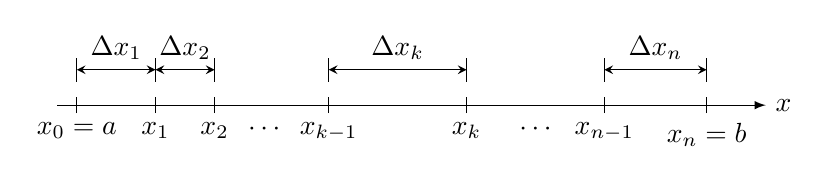
\begin{tikzpicture}
\draw[-latex](-0.25,0)--(8.75,0)node[right]{$x$};
\foreach \x/\s in {0/x_0=a,1/x_1,1.75/x_2,3.2/x_{k-1},4.95/x_k,6.7/x_{n-1},8/x_{n}=b}{\draw(\x,-0.1)node[below]{$\s$}--++(0,0.2); \draw(\x,0.3)--++(0,0.3);}
\draw(2.38,-0.1)node[below]{$\cdots$};
\draw(5.825,-0.1)node[below]{$\cdots$};
\foreach \xa/\xb/\s in {0/1/1,1/1.75/2,3.2/4.95/k,6.7/8/n}{\draw[stealth-stealth](\xa,0.45)--(\xb,0.45)node[pos=0.5,above]{$\Delta x_{\s}$};}
\end{tikzpicture}
\end{center}
ہر ذیلی وقفہ \عددی{[x_{k-1},x_k]} میں ہم کوئی نقطہ \عددی{c_k} منتخب کرتے ہوئے ذیلی وقفہ میں تفاعل \عددی{y=f(x)} پر نقطہ \عددی{(c_k,f(c_k))} تک مستطیل بناتے ہیں۔ جب تک نقطہ \عددی{c_k} ذیلی وقفہ \عددی{[x_{k-1},x_k]} میں پایا جاتا ہو اس کا مقام غیر اہم ہے (شکل \حوالہ{شکل_تکمل_رقبہ_بذریعہ_مستطیل_الف})۔

اگر \عددی{f(c_k)} مثبت ہو تب عدد \عددی{f(c_k)\Delta x_k} مستطیل کے قد ضرب قاعدہ یعنی مستطیل کے رقبہ کے برابر ہو گا۔ اگر \عددی{f(c_k)} منفی عدد ہو تب \عددی{f(c_k)\Delta x_k} مستطیل کے رقبہ کے نفی کے برابر ہو گا۔ ہم ان تمام \عددی{f(c_k)\Delta x_k} حاصل ضرب جن کی تعداد \عددی{n} ہے کا مجموعہ لیتے ہیں۔
\begin{align*}
S_P=\sum\limits_{k=1}^nf(c_k)\Delta x_k
\end{align*}
یہ مجموعہ جو \عددی{P} اور \عددی{c_k} کی انتخاب پر منحصر ہے وقفہ \عددی{[a,b]} پر \عددی{f} کا \اصطلاح{ریمان مجموعہ}\فرہنگ{ریمان!مجموعہ}\حاشیہب{Riemann sum}\فرہنگ{Riemann!sum} کہلاتا\حاشیہد{جرمنی کے ریاضی دان برنہارڈ ریمان [1826-1866] نے ایسے مجموعوں کی تحدیدی قیمتوں پر کام کیا۔} ہے۔

\عددی{[a,b]} کے خانوں کی چوڑائی کم سے کم کرتے ہوئے خانہ بندی سے حاصل مستطیل تفاعل \عددی{f} اور \عددی{x} محور کے بیچ خطہ کو بہتر سے بہتر  ظاہر کرتے ہیں (شکل \حوالہ{شکل_تکمل_زیادہ_ٹکڑے_بہتر_رقبہ} کا شکل \حوالہ{شکل_تکمل_رقبہ_بذریعہ_مستطیل_الف} کے ساتھ موازنہ کریں)۔یوں ہم توقع کرتے ہیں کہ ریمان مجموعہ کی تحدیدی  قیمت پائی جائے گی۔ ہماری اس توقع کو پرکھنے کی خاطر ہمیں خانوں کی چوڑائی کم سے کم کرنے کو ریاضیاتی صورت میں لکھنا ہو گا اور جاننا ہو گا کہ آیا مطابقتی مجموعہ کی کوئی تحدیدی قیمت پائی جاتی ہے۔ ہم درج ذیل تعریف کی مدد سے ایسا کر پائیں گے۔
\begin{figure}
\centering
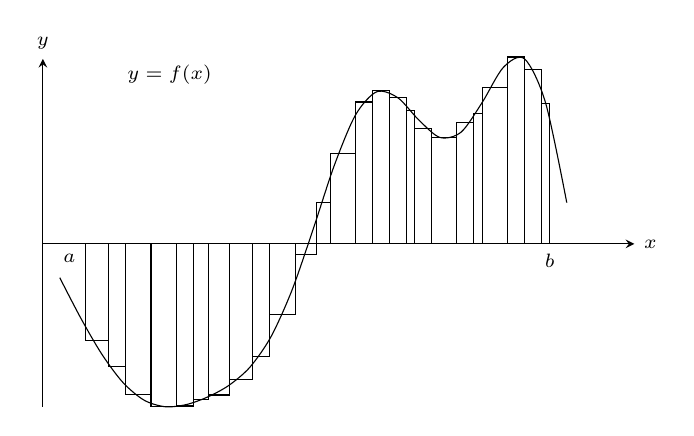
\begin{tikzpicture}[font=\small,declare function={f(\x)=-sin(deg(\x))-1/6*(\x/pi)^2*sin(deg(3*\x));}]
\begin{axis}[axis on top,clip=false,width=0.75*\textwidth,height=6cm,font=\scriptsize,axis lines=middle,xmin=0,xtick={\empty},ytick={\empty},xmax=7,xlabel={$x$},ylabel={$y$},xlabel style={at={(current axis.right of origin)},anchor=west},ylabel style={at={(current axis.above origin)},anchor=south}]
\addplot[domain=0.2:6.2,smooth]{f(x)};
\draw(axis cs:0.5,0)--(axis cs:0.5,{f(0.6)})--(axis cs:0.78,{f(0.6)})--(axis cs:0.78,0);
\draw(axis cs:0.78,0)--(axis cs:0.78,{f(0.8)})--(axis cs:0.98,{f(0.8)})--(axis cs:0.98,0);
\draw(axis cs:0.98,0)--(axis cs:0.98,{f(1.1)})--(axis cs:1.28,{f(1.1)})--(axis cs:1.28,0);
\draw(axis cs:1.28,0)--(axis cs:1.28,{f(1.48)})--(axis cs:1.58,{f(1.48)})--(axis cs:1.58,0);
\draw(axis cs:1.58,0)--(axis cs:1.58,{f(1.62)})--(axis cs:1.78,{f(1.62)})--(axis cs:1.78,0);
\draw(axis cs:1.78,0)--(axis cs:1.78,{f(1.88)})--(axis cs:1.96,{f(1.88)})--(axis cs:1.96,0);
\draw(axis cs:1.96,0)--(axis cs:1.96,{f(2)})--(axis cs:2.21,{f(2)})--(axis cs:2.21,0);
\draw(axis cs:2.21,0)--(axis cs:2.21,{f(2.3)})--(axis cs:2.485,{f(2.3)})--(axis cs:2.485,0);
\draw(axis cs:2.485,0)--(axis cs:2.485,{f(2.55)})--(axis cs:2.685,{f(2.55)})--(axis cs:2.685,0);
\draw(axis cs:2.685,0)--(axis cs:2.685,{f(2.83)})--(axis cs:2.985,{f(2.83)})--(axis cs:2.985,0);
\draw(axis cs:2.985,0)--(axis cs:2.985,{f(3.1)})--(axis cs:3.235,{f(3.1)})--(axis cs:3.235,0);
\draw(axis cs:3.235,0)--(axis cs:3.235,{f(3.3)})--(axis cs:3.4,{f(3.3)})--(axis cs:3.4,0);
\draw(axis cs:3.4,0)--(axis cs:3.4,{f(3.5)})--(axis cs:3.7,{f(3.5)})--(axis cs:3.7,0);
\draw(axis cs:3.7,0)--(axis cs:3.7,{f(3.8)})--(axis cs:3.9,{f(3.8)})--(axis cs:3.9,0);
\draw(axis cs:3.9,0)--(axis cs:3.9,{f(4)})--(axis cs:4.1,{f(4)})--(axis cs:4.1,0);
\draw(axis cs:4.1,0)--(axis cs:4.1,{f(4.2)})--(axis cs:4.3,{f(4.2)})--(axis cs:4.3,0);
\draw(axis cs:4.3,0)--(axis cs:4.3,{f(4.35)})--(axis cs:4.4,{f(4.35)})--(axis cs:4.4,0);
\draw(axis cs:4.4,0)--(axis cs:4.4,{f(4.55)})--(axis cs:4.6,{f(4.55)})--(axis cs:4.6,0);
\draw(axis cs:4.6,0)--(axis cs:4.6,{f(4.7)})--(axis cs:4.9,{f(4.7)})--(axis cs:4.9,0);
\draw(axis cs:4.9,0)--(axis cs:4.9,{f(5.05)})--(axis cs:5.1,{f(5.05)})--(axis cs:5.1,0);
\draw(axis cs:5.1,0)--(axis cs:5.1,{f(5.12)})--(axis cs:5.2,{f(5.12)})--(axis cs:5.2,0);
\draw(axis cs:5.2,0)--(axis cs:5.2,{f(5.3)})--(axis cs:5.5,{f(5.3)})--(axis cs:5.5,0);
\draw(axis cs:5.5,0)--(axis cs:5.5,{f(5.6)})--(axis cs:5.7,{f(5.6)})--(axis cs:5.7,0);
\draw(axis cs:5.7,0)--(axis cs:5.7,{f(5.8)})--(axis cs:5.9,{f(5.8)})--(axis cs:5.9,0);
\draw(axis cs:5.9,0)--(axis cs:5.9,{f(5.95)})--(axis cs:6.0,{f(5.95)})--(axis cs:6.0,0);
\draw(axis cs:0.5,0)node[below left]{$a$};
\draw(axis cs:6,0)node[below]{$b$};
\draw(axis cs:1.5,1)node[]{$y=f(x)$};
\end{axis}
\end{tikzpicture}
\caption{وقفہ $[a,b]$ کے زیادہ باریک خانہ بندی سے مستطیلوں کی تعداد بڑھتی ہے جن کے قاعدہ نسبتاً چھوٹے ہوتے ہیں۔}
\label{شکل_تکمل_زیادہ_ٹکڑے_بہتر_رقبہ}
\end{figure}

خانہ بندی \عددی{P} کی \اصطلاح{معیار}\فرہنگ{معیار}\حاشیہب{norm}\فرہنگ{norm} سے مراد سب سے لمبے خانے کی لمبائی ہے جس کو درج ذیل علامت سے ظاہر کیا جاتا ہے۔
\begin{align*}
&\norm{P} &&\text{\RL{(اس کو "$P$ کا معیار" پڑھیں)}}
\end{align*}
خانوں کی چوڑائی کم سے کم کرنے  کی بجائے اب ہم کہتے ہیں کہ خانوں کی معیار صفر تک پہنچائی جاتی ہے۔جیسے جیسے معیار کی قیمت صفر کے نزدیک ہوتی جاتی ہے ویسے ویسے ذیلی وقفوں کی لمبائی کم سے کم اور ان کی تعداد زیادہ سے زیادہ ہوتی جاتی ہے۔ خانوں کی چوڑائی کم کرنے سے باریک مستطیل پیدا ہوں گے۔

\ابتدا{مثال}
وقفہ \عددی{[0,2]} کی خانہ بندی  سلسلہ \عددی{P=\{0,0.2,0.6,1,1.5,2\}} ہے۔ \عددی{P} کے  پانچ ذیلی وقفے درج ذیل ہیں۔
\begin{align*}
[0,0.2],\,[0.2,0.6],\,[0.6,1],\,[1,1.5],\,[1.5,2]
\end{align*} 
ان ذیلی وقفوں کی لمبائیاں \عددی{\Delta x_1=0.2}، \عددی{\Delta x_2=0.4}، \عددی{\Delta x_3=0.4}، \عددی{\Delta x_4=0.5} اور \عددی{\Delta x_5=0.5} ہیں۔ ان میں سب سے لمبے ذیلی وقفہ کی لمبائی \عددی{0.5} ہے لہٰذا خانہ بندی \عددی{P} کا معیار \عددی{\norm{P}=0.5} ہے۔ اس مثال میں دو ذیلی وقفوں کی لمبائی \عددی{0.5} ہے۔
\انتہا{مثال}
%===========================

\ابتدا{تعریف}\موٹا{قطعی تکمل بطور ریمان مجموعوں کا حد}\\
فرض کریں وقفہ \عددی{[a,b]} پر \عددی{f(x)} ایک معین تفاعل ہے۔ ہم کہتے ہیں کہ \عددی{\norm{P}\to 0} کرتے ہوئے وقفہ \عددی{[a,b]} پر ریمان مجموعہ \عددی{\sum_{k=1}^nf(c_k)\Delta x_k} کا حد اس صورت عدد \عددی{I} ہو گا جب درج ذیل شرط پورا ہوتا ہو:

کسی بھی دیے گئے عدد \عددی{\epsilon>0} کے لئے ایسا مطابقتی عدد \عددی{\delta>0} موجود ہے کہ ذیلی وقفہ \عددی{[x_{k-1},x_k]} میں کسی بھی منتخب عدد \عددی{c_k} کے لئے  درج ذیل مطمئن ہو۔
\begin{align*}
\norm{P}<\delta\quad\implies\quad \abs{\sum\limits_{k=1}^n f(c_k)\Delta x_k}<\epsilon
\end{align*}
\انتہا{تعریف}

اگر یہ حد موجود ہو تب ہم  درج ذیل لکھتے ہیں۔
\begin{align*}
\lim_{\norm{P}\to 0}\sum\limits_{k=1}^n f(c_k)\Delta x_k=I
\end{align*}
وقفہ \عددی{[a,b]} پر  عدد \عددی{I} تفاعل  \عددی{f} کا \اصطلاح{قطعی تکمل}\فرہنگ{قطعی!تکمل}\فرہنگ{تکمل!قطعی}\حاشیہب{definite integral}\فرہنگ{integral!definite} کہلاتا ہے، اور ہم کہتے ہیں کہ \عددی{[a,b]} پر \عددی{f} \اصطلاح{قابل تکمل}\فرہنگ{تکمل!قابل}\حاشیہب{integrable}\فرہنگ{integrable} ہے اور \عددی{[a,b]} پر \عددی{f} کا ریمان مجموعہ عدد \عددی{I} پر \اصطلاح{مرکوز}\فرہنگ{مرکوز}\حاشیہب{converges}\فرہنگ{converges} ہے۔

ہم عموماً \عددی{I} کو \عددی{\int_a^bf(x)\dif x} لکھتے ہیں جو "\عددی{a} تا \عددی{b} تفاعل \عددی{f} کا تکمل" پڑھا جاتا ہے۔یوں اگر حد موجود ہو تب درج ذیل لکھا جائے گا۔
\begin{align*}
\lim_{\norm{P}\to 0}\sum\limits_{k=1}^nf(c_k)\Delta x_k=\int_a^bf(x)\dif x
\end{align*}

دلچسپ حقیقت یہ ہے کہ خانہ بندی تبدیل کرتے ہوئے اور ہر خانے میں \عددی{c_k} کا مقام تبدیل کرنے کے باوجود استمراری \عددی{f} کی صورت میں  \عددی{\norm{P}\to 0} کرتے ہوئے ریمان مجموعوں \عددی{\sum f(c_k)\Delta x_k} کی تحدیدی قیمت تبدیل نہیں ہوتی ہے۔ریمان نے \سن{1854} میں درج ذیل مسئلہ ثابت کرتے ہوئے اس حقیقت کی تصدیق کر دی۔ ریمان کے ثبوت کی جدید صورت احصاء کی تقریباً تمام اعلٰی  کتابوں میں پایا جاتا ہے۔

\ابتدا{مسئلہ}\شناخت{مسئلہ_تکمل_قطعی_تکمل_کی_موجودگی}\موٹا{قطعی تکمل کی موجودگی}\\
تمام استمراری تفاعل قابل تکمل ہیں۔ یعنی وقفہ \عددی{[a,b]} پر استمراری تفاعل \عددی{f} کا \عددی{[a,b]} پر قطعی تکمل موجود ہو گا۔
\انتہا{مسئلہ}
%===================

ہم کیوں یقین کریں کہ یہ مسئلہ کار آمد ہو گا؟ وقفہ \عددی{[a,b]} کی عمومی خانہ بندی \عددی{P} فرض کریں۔ چونکہ تفاعل \عددی{f} استمراری ہے لہٰذا ہر ذیلی وقفہ پر اس کی کوئی کم سے کم قیمت  \عددی{k_L} اور کوئی زیادہ سے زیادہ قیمت \عددی{k_H} ہو گی۔ کم سے کم قیمتوں (شکل \حوالہ{شکل_تکمل_فرق_بالائی_زیریں_مجموعہ}-ا) سے حاصل ضرب \عددی{k_L\Delta x_k} کا درج ذیل مجموعہ \عددی{P} پر \عددی{f} کا \اصطلاح{زیریں مجموعہ}\فرہنگ{مجموعہ!زیریں}\حاشیہب{lower sum}\فرہنگ{sum!lower} \عددی{L} کہلاتا ہے۔
\begin{align*}
L=k_{L1}\Delta x_1+k_{L2}\Delta x_2+\cdots+k_{Ln}\Delta x_n
\end{align*}
اسی طرح  زیادہ سے زیادہ قیمتوں (شکل \حوالہ{شکل_تکمل_فرق_بالائی_زیریں_مجموعہ}-ب) سے حاصل ضرب \عددی{k_H\Delta x_k} کا درج ذیل مجموعہ \عددی{P} پر \عددی{f} کا بالائی مجموعہ \عددی{H} کہلاتا ہے۔
\begin{align*}
H=k_{H1}\Delta x_1+k_{H2}\Delta x_2+\cdots+k_{Hn}\Delta x_n
\end{align*}
ان کا فرق \عددی{H-L} شکل \حوالہ{شکل_تکمل_فرق_بالائی_زیریں_مجموعہ}-ج میں دکھائے گیے سیاہ ڈبوں کے رقبہ کے برابر ہو گا۔جیسا جیسا \عددی{\norm{P}\to 0} کیا جائے ان ڈبوں کی تعداد بڑھتی جائے گی جبکہ ان کی چوڑائی اور لمبائی کم سے کم ہوتی جائے گی۔ ہم \عددی{\norm{P}} کو صفر کے کافی نزدیک کرتے ہوئے غیر منفی عدد \عددی{H-L} کو کسی بھی چھوٹے سے چھوٹے مثبت عدد \عددی{\epsilon} سے کم کر سکتے ہیں، یعنی
\begin{align}\label{مساوات_تکمل_ڈبوں_رقبہ_الف}
\lim_{\norm{P}\to 0}(H-L)=0
\end{align}
اور جیسا اعلٰی  نصاب میں دکھایا گیا ہے  درج بالا سے مراد درج ذیل ہے۔
\begin{align}\label{مساوات_تکمل_ڈبوں_رقبہ_ب}
\lim_{\norm{P}\to 0}L=\lim_{\norm{P}\to0}H
\end{align}
بند  وقفوں پر استمراری تفاعل کی ایک خاصیت جس کو \اصطلاح{یکساں استمرار}\فرہنگ{استمرار!یکساں}\حاشیہب{uniform continuity}\فرہنگ{continuity!uniform} کہتے ہیں کی بدولت مساوات \حوالہ{مساوات_تکمل_ڈبوں_رقبہ_الف} اور مساوات \حوالہ{مساوات_تکمل_ڈبوں_رقبہ_ب} کار آمد ہیں۔ یہ خاصیت ممکن بناتی ہے کہ \عددی{\norm{P}\to 0} کرتے ہوئے ان ڈبوں، جو \عددی{H} اور \عددی{L} کے فرق کو ظاہر کرتے ہیں،  کی چوڑائی کو کم سے کم کرتے ہوئے ان کی قد کو کم سے کم بنایا جا سکتا ہے اور ہم ان کی چوڑائی کم کرتے ہوئے ان کے قد کو جتنا چاہیں کم کر سکتے ہیں۔ چونکہ یکساں استمرار سے منسلک \عددی{\epsilon} بالمقابل \عددی{\delta} کی دلیل ہم نے یہاں پیش نہیں کی ہے لہٰذا ہم مساوات  \حوالہ{مساوات_تکمل_ڈبوں_رقبہ_ب} کو ثبوت نہیں مان سکتے ہیں البتہ مذکورہ بالا دلائل اصل ثبوت کی روح پیش کرتے ہیں۔

ہم  وقفہ \عددی{[a,b]} پر استمراری تفاعل \عددی{f} کے لئے مساوات \حوالہ{مساوات_تکمل_ڈبوں_رقبہ_ب} کو درست تصور کرتے ہوئے  \عددی{P} کے ہر  ذیلی وقفہ \عددی{[x_{k-1},x_k]} پر نقطہ \عددی{c_k} منتخب کرتے ہوئے  ریمان مجموعہ \عددی{\sum_{k=1}^nf(c_k)\Delta x_k} لکھتے ہیں. اب ہر \عددی{k} کے لئے \عددی{k_L\le f(c_k)\le k_H} ہو گا لہٰذا درج ذیل لکھا جا سکتا ہے۔
\begin{align*}
L\le \sum\limits_{k=1}^nf(c_k)\Delta x_k\le H
\end{align*}
\عددی{f} کا ریمان مجموعہ \عددی{H} اور \عددی{L} کے بیچ پایا جاتا ہے۔مسئلہ بیچ (مسئلہ \حوالہ{مسئلہ_حد_بیچ})  کی ترمیم شدہ روپ سے ہم اخذ کرتے ہیں کہ \عددی{\norm{P}\to0} کرتے ہوئے ریمان مجموعہ کا حد موجود ہو گا اور یہ \عددی{L} اور \عددی{H} کی مشترکہ تحدیدی قیمت ہو گی:
\begin{align*}
\lim_{\norm{P}\to0}L=\lim_{\norm{P}\to0}\sum\limits_{k=1}^nf(c_k)\Delta x_k=\lim_{\norm{P}\to0}H
\end{align*}

ایک لمحہ رک کر اس نتیجہ پر غور کریں۔اس نتیجہ کے تحت ہم \عددی{c_k} کو جس طرح بھی منتخب کریں، \عددی{\norm{P}\to 0} کرتے ہوئے ریمان مجموعہ کی تحدیدی قیمت وہی حاصل ہو گی۔ ہر \عددی{f(c_k)} کو \عددی{[x_{k-1},x_k]} پر \عددی{f} کی کم سے کم قیمت منتخب کر کے وہی حد حاصل ہو گا۔ اسی طرح ہر \عددی{f(c_k)} کو \عددی{[x_{k-1},x_k]} پر \عددی{f} کی زیادہ سے زیادہ  قیمت منتخب کر کے بھی وہی حد حاصل ہو گا۔  \عددی{c_k} کو بلا منصوبہ منتخب کر کے بھی یہی حد حاصل ہو گا۔

اگرچہ ہم نے قطعی تکمل کی موجودگی کا مسئلہ بالخصوص استمراری تفاعل کے لئے پیش کیا، حقیقت میں کئی غیر استمراری تفاعل بھی قابل تکمل ہیں۔غیر محدود تفاعل کی تکمل پر اسی باب میں غور کیا جائے گا۔

\begin{figure}
\centering
\begin{subfigure}{0.45\textwidth}
\centering
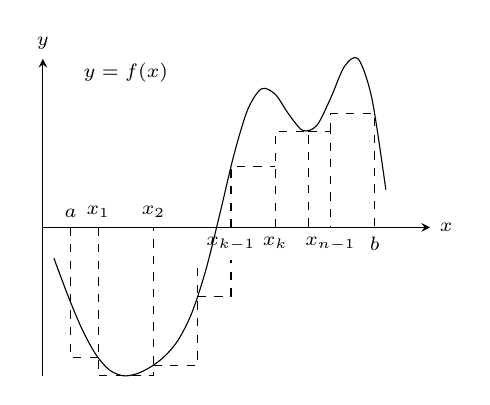
\begin{tikzpicture}[font=\small,declare function={f(\x)=-sin(deg(\x))-1/6*(\x/pi)^2*sin(deg(3*\x));}]
\pgfmathsetmacro{\xx}{0.5}
\pgfmathsetmacro{\xa}{1}
\pgfmathsetmacro{\xb}{2}
\pgfmathsetmacro{\xc}{2.8}
\pgfmathsetmacro{\xd}{3.4}
\pgfmathsetmacro{\xe}{4.2}
\pgfmathsetmacro{\xf}{4.8}
\pgfmathsetmacro{\xg}{5.2}
\pgfmathsetmacro{\xh}{6}
\pgfmathsetmacro{\ca}{\xa}
\pgfmathsetmacro{\cb}{1.5}
\pgfmathsetmacro{\cc}{\xb}
\pgfmathsetmacro{\cd}{\xc}
\pgfmathsetmacro{\ce}{\xd}
\pgfmathsetmacro{\cf}{\xf}
\pgfmathsetmacro{\cg}{\xf}
\pgfmathsetmacro{\ch}{\xh}
\pgfmathsetmacro{\pa}{f(\ca)}
\pgfmathsetmacro{\pb}{f(\cb)}
\pgfmathsetmacro{\pc}{f(\cc)}
\pgfmathsetmacro{\pd}{f(\cd)}
\pgfmathsetmacro{\pe}{f(\ce)}
\pgfmathsetmacro{\pf}{f(\cf)}
\pgfmathsetmacro{\pg}{f(\cg)}
\pgfmathsetmacro{\ph}{f(\ch)}
\begin{axis}[axis on top,clip=false,small,font=\scriptsize,axis lines=middle,xmin=0,xtick={\empty},ytick={\empty},xmax=7,xlabel={$x$},ylabel={$y$},xlabel style={at={(current axis.right of origin)},anchor=west},ylabel style={at={(current axis.above origin)},anchor=south}]
%\addplot[domain=0.2:6.2,smooth]{f(x)};
\draw[dashed](axis cs:\xx,0)node[above]{$a$}--(axis cs:\xx,\pa)--(axis cs:\xa,\pa);
\draw[dashed](axis cs:\xa,0)node[above]{$x_1$}--(axis cs:\xa,\pb)--(axis cs:\xb,\pb)--(axis cs:\xb,0)node[above]{$x_2$};
\draw[dashed](axis cs:\xb,\pc)--(axis cs:\xc,\pc)--(axis cs:\xc,0);
\draw[dashed](axis cs:\xc,\pd)--(axis cs:\xd,\pd)--(axis cs:\xd,0)node[below,fill=white]{$x_{k-1}$};
\draw[dashed](axis cs:\xd,0)--(axis cs:\xd,\pe)--(axis cs:\xe,\pe);
\draw[dashed](axis cs:\xe,0)node[below,fill=white]{$x_k$}--(axis cs:\xe,\pf)--(axis cs:\xf,\pf)--(axis cs:\xf,0);
\draw[dashed](axis cs:\xf,\pg)--(axis cs:\xg,\pg)--(axis cs:\xg,0)node[below]{$x_{n-1}$};
\draw[dashed](axis cs:\xg,\pg)--(axis cs:\xg,\ph)--(axis cs:\xh,\ph)--(axis cs:\xh,0)node[below]{$b$};
\draw(axis cs:1.5,1)node[]{$y=f(x)$};
\addplot[domain=0.2:6.2,smooth]{f(x)};
\end{axis}
\end{tikzpicture}
\caption{زیریں مجموعہ \عددی{L=\sum\limits_{k=1}^nk_L\Delta x_k}}
\end{subfigure}\hfill
\begin{subfigure}{0.45\textwidth}
\centering
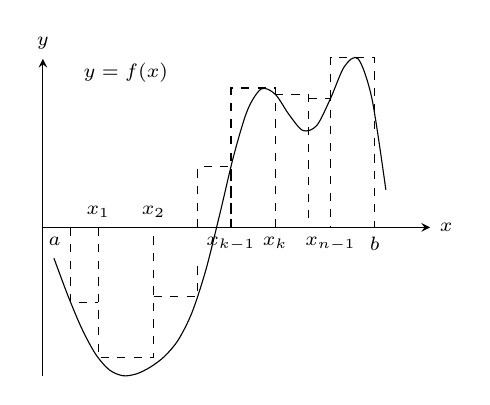
\begin{tikzpicture}[font=\small,declare function={f(\x)=-sin(deg(\x))-1/6*(\x/pi)^2*sin(deg(3*\x));}]
\pgfmathsetmacro{\xx}{0.5}
\pgfmathsetmacro{\xa}{1}
\pgfmathsetmacro{\xb}{2}
\pgfmathsetmacro{\xc}{2.8}
\pgfmathsetmacro{\xd}{3.4}
\pgfmathsetmacro{\xe}{4.2}
\pgfmathsetmacro{\xf}{4.8}
\pgfmathsetmacro{\xg}{5.2}
\pgfmathsetmacro{\xh}{6}
\pgfmathsetmacro{\ca}{\xx}
\pgfmathsetmacro{\cb}{\xa}
\pgfmathsetmacro{\cc}{\xc}
\pgfmathsetmacro{\cd}{\xd}
\pgfmathsetmacro{\ce}{\xe}
\pgfmathsetmacro{\cf}{\xe}
\pgfmathsetmacro{\cg}{\xg}
\pgfmathsetmacro{\ch}{\xg}
\pgfmathsetmacro{\pa}{f(\ca)}
\pgfmathsetmacro{\pb}{f(\cb)}
\pgfmathsetmacro{\pc}{f(\cc)}
\pgfmathsetmacro{\pd}{f(\cd)}
\pgfmathsetmacro{\pe}{f(\ce)}
\pgfmathsetmacro{\pf}{f(\cf)}
\pgfmathsetmacro{\pg}{f(\cg)}
\pgfmathsetmacro{\ph}{f(\ch)}
\begin{axis}[axis on top,clip=false,small,font=\scriptsize,axis lines=middle,xmin=0,xtick={\empty},ytick={\empty},xmax=7,xlabel={$x$},ylabel={$y$},xlabel style={at={(current axis.right of origin)},anchor=west},ylabel style={at={(current axis.above origin)},anchor=south}]
%\addplot[domain=0.2:6.2,smooth]{f(x)};
\draw[dashed](axis cs:\xx,0)node[below left]{$a$}--(axis cs:\xx,\pa)--(axis cs:\xa,\pa);
\draw[dashed](axis cs:\xa,0)node[above]{$x_1$}--(axis cs:\xa,\pb)--(axis cs:\xb,\pb)--(axis cs:\xb,0)node[above]{$x_2$};
\draw[dashed](axis cs:\xb,\pc)--(axis cs:\xc,\pc)--(axis cs:\xc,0);
\draw[dashed](axis cs:\xc,0)--(axis cs:\xc,\pd)--(axis cs:\xd,\pd)--(axis cs:\xd,0)node[below,fill=white]{$x_{k-1}$};
\draw[dashed](axis cs:\xd,0)--(axis cs:\xd,{f(4)})--(axis cs:\xe,{f(4)})--(axis cs:\xe,\pe);
\draw[dashed](axis cs:\xe,0)node[below,fill=white]{$x_k$}--(axis cs:\xe,\pf)--(axis cs:\xf,\pf)--(axis cs:\xf,0);
\draw[dashed](axis cs:\xf,\pg)--(axis cs:\xg,\pg)--(axis cs:\xg,0)node[below]{$x_{n-1}$};
\draw[dashed](axis cs:\xg,\pg)--(axis cs:\xg,{f(5.6)})--(axis cs:\xh,{f(5.6)})--(axis cs:\xh,0)node[below]{$b$};
\addplot[domain=0.2:6.2,smooth]{f(x)};
\draw(axis cs:1.5,1)node[]{$y=f(x)$};
\end{axis}
\end{tikzpicture}
\caption{بالائی مجموعہ \عددی{H=\sum\limits_{k=1}^nk_H\Delta x_k}}
\end{subfigure}
\begin{subfigure}{0.45\textwidth}
\centering
\begin{tikzpicture}[font=\small,declare function={f(\x)=-sin(deg(\x))-1/6*(\x/pi)^2*sin(deg(3*\x));}]
\pgfmathsetmacro{\xx}{0.5}
\pgfmathsetmacro{\xa}{1}
\pgfmathsetmacro{\xb}{2}
\pgfmathsetmacro{\xc}{2.8}
\pgfmathsetmacro{\xd}{3.4}
\pgfmathsetmacro{\xe}{4.2}
\pgfmathsetmacro{\xf}{4.8}
\pgfmathsetmacro{\xg}{5.2}
\pgfmathsetmacro{\xh}{6}
\pgfmathsetmacro{\ca}{\xx}
\pgfmathsetmacro{\cb}{\xa}
\pgfmathsetmacro{\cc}{\xc}
\pgfmathsetmacro{\cd}{\xd}
\pgfmathsetmacro{\ce}{\xe}
\pgfmathsetmacro{\cf}{\xe}
\pgfmathsetmacro{\cg}{\xg}
\pgfmathsetmacro{\ch}{\xg}
\pgfmathsetmacro{\pa}{f(\ca)}
\pgfmathsetmacro{\pb}{f(\cb)}
\pgfmathsetmacro{\pc}{f(\cc)}
\pgfmathsetmacro{\pd}{f(\cd)}
\pgfmathsetmacro{\pe}{f(\ce)}
\pgfmathsetmacro{\pf}{f(\cf)}
\pgfmathsetmacro{\pg}{f(\cg)}
\pgfmathsetmacro{\ph}{f(\ch)}
\begin{axis}[axis on top,clip=false,small,font=\scriptsize,axis lines=middle,xmin=0,xtick={\empty},ytick={\empty},xmax=7,xlabel={$x$},ylabel={$y$},xlabel style={at={(current axis.right of origin)},anchor=west},ylabel style={at={(current axis.above origin)},anchor=south}]
%\addplot[domain=0.2:6.2,smooth]{f(x)};
\draw[fill=lgray](axis cs:\xx,{f(\xx)})--(axis cs:\xx,{f(\xa)})--(axis cs:\xa,{f(\xa)})--(axis cs:\xa,{f(\xx)})--(axis cs:\xx,{f(\xx)});
\draw[fill=lgray](axis cs:\xa,{f(\xa)})--(axis cs:\xa,{f(1.5)})--(axis cs:\xb,{f(1.5)})--(axis cs:\xb,{f(\xa)})--(axis cs:\xa,{f(\xa)});
\draw[fill=lgray](axis cs:\xb,{f(\xc)})--(axis cs:\xb,{f(\xb)})--(axis cs:\xc,{f(\xb)})--(axis cs:\xc,{f(\xc)})--(axis cs:\xb,{f(\xc)});
\draw[fill=lgray](axis cs:\xc,{f(\xd)})--(axis cs:\xc,{f(\xc)})--(axis cs:\xd,{f(\xc)})--(axis cs:\xd,{f(\xd)})--(axis cs:\xc,{f(\xd)});
\draw[fill=lgray](axis cs:\xd,{f(4)})--(axis cs:\xd,{f(\xd)})--(axis cs:\xe,{f(\xd)})--(axis cs:\xe,{f(4)})--(axis cs:\xd,{f(4)});
\draw[fill=lgray](axis cs:\xe,{f(\xe)})--(axis cs:\xe,{f(\xf)})--(axis cs:\xf,{f(\xf)})--(axis cs:\xf,{f(\xe)})--(axis cs:\xe,{f(\xe)});
\draw[fill=lgray](axis cs:\xf,{f(\xg)})--(axis cs:\xf,{f(\xf)})--(axis cs:\xg,{f(\xf)})--(axis cs:\xg,{f(\xg)})--(axis cs:\xf,{f(\xg)});
\draw[fill=lgray](axis cs:\xg,{f(5.6)})--(axis cs:\xg,{f(\xh)})--(axis cs:\xh,{f(\xh)})--(axis cs:\xh,{f(5.6)})--(axis cs:\xg,{f(5.6)});
\addplot[domain=0.2:6.2,smooth]{f(x)};
\draw(axis cs:\xx,0)node[above]{$x_0=a$}--(axis cs:\xx,{f(\xx)});
\draw(axis cs:\xh,0)node[below]{$x_n=b$}--(axis cs:\xh,{f(\xh)});
%
\begin{scope}[yshift=-4cm]
\draw[fill=lgray](axis cs:\xx,0)--(axis cs:\xx,{abs(f(\xx)-f(\xa))})--(axis cs:\xa,{abs(f(\xx)-f(\xa))})--(axis cs:\xa,0)--(axis cs:\xx,0);
\draw[fill=lgray](axis cs:\xa,0)--(axis cs:\xa,{abs(f(1.5)-f(\xa))})--(axis cs:\xb,{abs(f(1.5)-f(\xa))})--(axis cs:\xb,0)--(axis cs:\xa,0);
\draw[fill=lgray](axis cs:\xb,0)--(axis cs:\xb,{abs(f(\xb)-f(\xc))})--(axis cs:\xc,{abs(f(\xb)-f(\xc))})--(axis cs:\xc,0)--(axis cs:\xb,0);
\draw[fill=lgray](axis cs:\xc,0)--(axis cs:\xc,{abs(f(\xc)-f(\xd))})--(axis cs:\xd,{abs(f(\xc)-f(\xd))})--(axis cs:\xd,0)--(axis cs:\xc,0);
\draw[fill=lgray](axis cs:\xd,0)--(axis cs:\xd,{abs(f(\xd)-f(4))})--(axis cs:\xe,{abs(f(\xd)-f(4))})--(axis cs:\xe,0)--(axis cs:\xd,0);
\draw[fill=lgray](axis cs:\xe,0)--(axis cs:\xe,{abs(f(\xf)-f(\xe))})--(axis cs:\xf,{abs(f(\xf)-f(\xe))})--(axis cs:\xf,0)--(axis cs:\xe,0);
\draw[fill=lgray](axis cs:\xf,0)--(axis cs:\xf,{abs(f(\xf)-f(\xg))})--(axis cs:\xg,{abs(f(\xf)-f(\xg))})--(axis cs:\xg,0)--(axis cs:\xf,0);
\draw[fill=lgray](axis cs:\xg,0)--(axis cs:\xg,{abs(f(\xh)-f(5.6))})--(axis cs:\xh,{abs(f(\xh)-f(5.6))})--(axis cs:\xh,0)--(axis cs:\xg,0);
\draw(axis cs:\xx,-0.1)--(axis cs:\xx,-0.4);
\draw(axis cs:\xh,-0.1)--(axis cs:\xh,-0.4);
\draw[stealth-stealth](axis cs:\xx,-0.3)--(axis cs:\xh,-0.3)node[pos=0.5,fill=white]{$b-a$};
\draw(axis cs:\xx,0)--(axis cs:\xx,{abs(f(\xc)-f(\xd+0.1))})--(axis cs:\xh,{abs(f(\xc)-f(\xd+0.1))})--(axis cs:\xh,0);
\draw(axis cs:\xx-0.2,0)--(axis cs:\xx-0.6,0);
\draw(axis cs:\xx-0.2,{abs(f(\xc)-f(\xd+0.1))})--(axis cs:\xx-0.6,{abs(f(\xc)-f(\xd+0.1))});
\draw[stealth-stealth](axis cs:\xx-0.4,0)--(axis cs:\xx-0.4,{abs(f(\xc)-f(\xd+0.1))})node[pos=0.5,left]{$\epsilon'=\frac{\epsilon}{b-a}$};
\end{scope}
\end{axis}
\end{tikzpicture}
\caption{فرق \عددی{H-L} کو \عددی{\epsilon'\cdot(b-a)} یعنی \عددی{\epsilon} سے کم بنایا جا سکتا ہے۔}
\end{subfigure}\hfill
\caption{بالائی اور زیریں مجموعوں میں فرق۔}
\label{شکل_تکمل_فرق_بالائی_زیریں_مجموعہ}
\end{figure}

